% Options for packages loaded elsewhere
\PassOptionsToPackage{unicode}{hyperref}
\PassOptionsToPackage{hyphens}{url}
%
\documentclass[
  12pt,
]{book}
\usepackage{amsmath,amssymb}
\usepackage{setspace}
\usepackage{iftex}
\ifPDFTeX
  \usepackage[T1]{fontenc}
  \usepackage[utf8]{inputenc}
  \usepackage{textcomp} % provide euro and other symbols
\else % if luatex or xetex
  \usepackage{unicode-math} % this also loads fontspec
  \defaultfontfeatures{Scale=MatchLowercase}
  \defaultfontfeatures[\rmfamily]{Ligatures=TeX,Scale=1}
\fi
\usepackage{lmodern}
\ifPDFTeX\else
  % xetex/luatex font selection
\fi
% Use upquote if available, for straight quotes in verbatim environments
\IfFileExists{upquote.sty}{\usepackage{upquote}}{}
\IfFileExists{microtype.sty}{% use microtype if available
  \usepackage[]{microtype}
  \UseMicrotypeSet[protrusion]{basicmath} % disable protrusion for tt fonts
}{}
\makeatletter
\@ifundefined{KOMAClassName}{% if non-KOMA class
  \IfFileExists{parskip.sty}{%
    \usepackage{parskip}
  }{% else
    \setlength{\parindent}{0pt}
    \setlength{\parskip}{6pt plus 2pt minus 1pt}}
}{% if KOMA class
  \KOMAoptions{parskip=half}}
\makeatother
\usepackage{xcolor}
\usepackage[top=1in,left=1in,right=1in,bottom=1in]{geometry}
\usepackage{color}
\usepackage{fancyvrb}
\newcommand{\VerbBar}{|}
\newcommand{\VERB}{\Verb[commandchars=\\\{\}]}
\DefineVerbatimEnvironment{Highlighting}{Verbatim}{commandchars=\\\{\}}
% Add ',fontsize=\small' for more characters per line
\usepackage{framed}
\definecolor{shadecolor}{RGB}{248,248,248}
\newenvironment{Shaded}{\begin{snugshade}}{\end{snugshade}}
\newcommand{\AlertTok}[1]{\textcolor[rgb]{0.94,0.16,0.16}{#1}}
\newcommand{\AnnotationTok}[1]{\textcolor[rgb]{0.56,0.35,0.01}{\textbf{\textit{#1}}}}
\newcommand{\AttributeTok}[1]{\textcolor[rgb]{0.13,0.29,0.53}{#1}}
\newcommand{\BaseNTok}[1]{\textcolor[rgb]{0.00,0.00,0.81}{#1}}
\newcommand{\BuiltInTok}[1]{#1}
\newcommand{\CharTok}[1]{\textcolor[rgb]{0.31,0.60,0.02}{#1}}
\newcommand{\CommentTok}[1]{\textcolor[rgb]{0.56,0.35,0.01}{\textit{#1}}}
\newcommand{\CommentVarTok}[1]{\textcolor[rgb]{0.56,0.35,0.01}{\textbf{\textit{#1}}}}
\newcommand{\ConstantTok}[1]{\textcolor[rgb]{0.56,0.35,0.01}{#1}}
\newcommand{\ControlFlowTok}[1]{\textcolor[rgb]{0.13,0.29,0.53}{\textbf{#1}}}
\newcommand{\DataTypeTok}[1]{\textcolor[rgb]{0.13,0.29,0.53}{#1}}
\newcommand{\DecValTok}[1]{\textcolor[rgb]{0.00,0.00,0.81}{#1}}
\newcommand{\DocumentationTok}[1]{\textcolor[rgb]{0.56,0.35,0.01}{\textbf{\textit{#1}}}}
\newcommand{\ErrorTok}[1]{\textcolor[rgb]{0.64,0.00,0.00}{\textbf{#1}}}
\newcommand{\ExtensionTok}[1]{#1}
\newcommand{\FloatTok}[1]{\textcolor[rgb]{0.00,0.00,0.81}{#1}}
\newcommand{\FunctionTok}[1]{\textcolor[rgb]{0.13,0.29,0.53}{\textbf{#1}}}
\newcommand{\ImportTok}[1]{#1}
\newcommand{\InformationTok}[1]{\textcolor[rgb]{0.56,0.35,0.01}{\textbf{\textit{#1}}}}
\newcommand{\KeywordTok}[1]{\textcolor[rgb]{0.13,0.29,0.53}{\textbf{#1}}}
\newcommand{\NormalTok}[1]{#1}
\newcommand{\OperatorTok}[1]{\textcolor[rgb]{0.81,0.36,0.00}{\textbf{#1}}}
\newcommand{\OtherTok}[1]{\textcolor[rgb]{0.56,0.35,0.01}{#1}}
\newcommand{\PreprocessorTok}[1]{\textcolor[rgb]{0.56,0.35,0.01}{\textit{#1}}}
\newcommand{\RegionMarkerTok}[1]{#1}
\newcommand{\SpecialCharTok}[1]{\textcolor[rgb]{0.81,0.36,0.00}{\textbf{#1}}}
\newcommand{\SpecialStringTok}[1]{\textcolor[rgb]{0.31,0.60,0.02}{#1}}
\newcommand{\StringTok}[1]{\textcolor[rgb]{0.31,0.60,0.02}{#1}}
\newcommand{\VariableTok}[1]{\textcolor[rgb]{0.00,0.00,0.00}{#1}}
\newcommand{\VerbatimStringTok}[1]{\textcolor[rgb]{0.31,0.60,0.02}{#1}}
\newcommand{\WarningTok}[1]{\textcolor[rgb]{0.56,0.35,0.01}{\textbf{\textit{#1}}}}
\usepackage{longtable,booktabs,array}
\usepackage{calc} % for calculating minipage widths
% Correct order of tables after \paragraph or \subparagraph
\usepackage{etoolbox}
\makeatletter
\patchcmd\longtable{\par}{\if@noskipsec\mbox{}\fi\par}{}{}
\makeatother
% Allow footnotes in longtable head/foot
\IfFileExists{footnotehyper.sty}{\usepackage{footnotehyper}}{\usepackage{footnote}}
\makesavenoteenv{longtable}
\usepackage{graphicx}
\makeatletter
\def\maxwidth{\ifdim\Gin@nat@width>\linewidth\linewidth\else\Gin@nat@width\fi}
\def\maxheight{\ifdim\Gin@nat@height>\textheight\textheight\else\Gin@nat@height\fi}
\makeatother
% Scale images if necessary, so that they will not overflow the page
% margins by default, and it is still possible to overwrite the defaults
% using explicit options in \includegraphics[width, height, ...]{}
\setkeys{Gin}{width=\maxwidth,height=\maxheight,keepaspectratio}
% Set default figure placement to htbp
\makeatletter
\def\fps@figure{htbp}
\makeatother
\setlength{\emergencystretch}{3em} % prevent overfull lines
\providecommand{\tightlist}{%
  \setlength{\itemsep}{0pt}\setlength{\parskip}{0pt}}
\setcounter{secnumdepth}{5}
\usepackage{booktabs}
\ifLuaTeX
  \usepackage{selnolig}  % disable illegal ligatures
\fi
\usepackage[]{natbib}
\bibliographystyle{apalike}
\IfFileExists{bookmark.sty}{\usepackage{bookmark}}{\usepackage{hyperref}}
\IfFileExists{xurl.sty}{\usepackage{xurl}}{} % add URL line breaks if available
\urlstyle{same}
\hypersetup{
  pdftitle={IOBR (Immuno-Oncology Biological Research)},
  pdfauthor={Dongqiang Zeng},
  hidelinks,
  pdfcreator={LaTeX via pandoc}}

\title{IOBR (Immuno-Oncology Biological Research)}
\author{Dongqiang Zeng}
\date{2023-08-25}

\begin{document}
\maketitle

{
\setcounter{tocdepth}{1}
\tableofcontents
}
\setstretch{1.2}
\hypertarget{introduction}{%
\chapter*{\texorpdfstring{\textbf{Introduction}}{Introduction}}\label{introduction}}
\addcontentsline{toc}{chapter}{\textbf{Introduction}}

Preface

\begin{figure}

{\centering 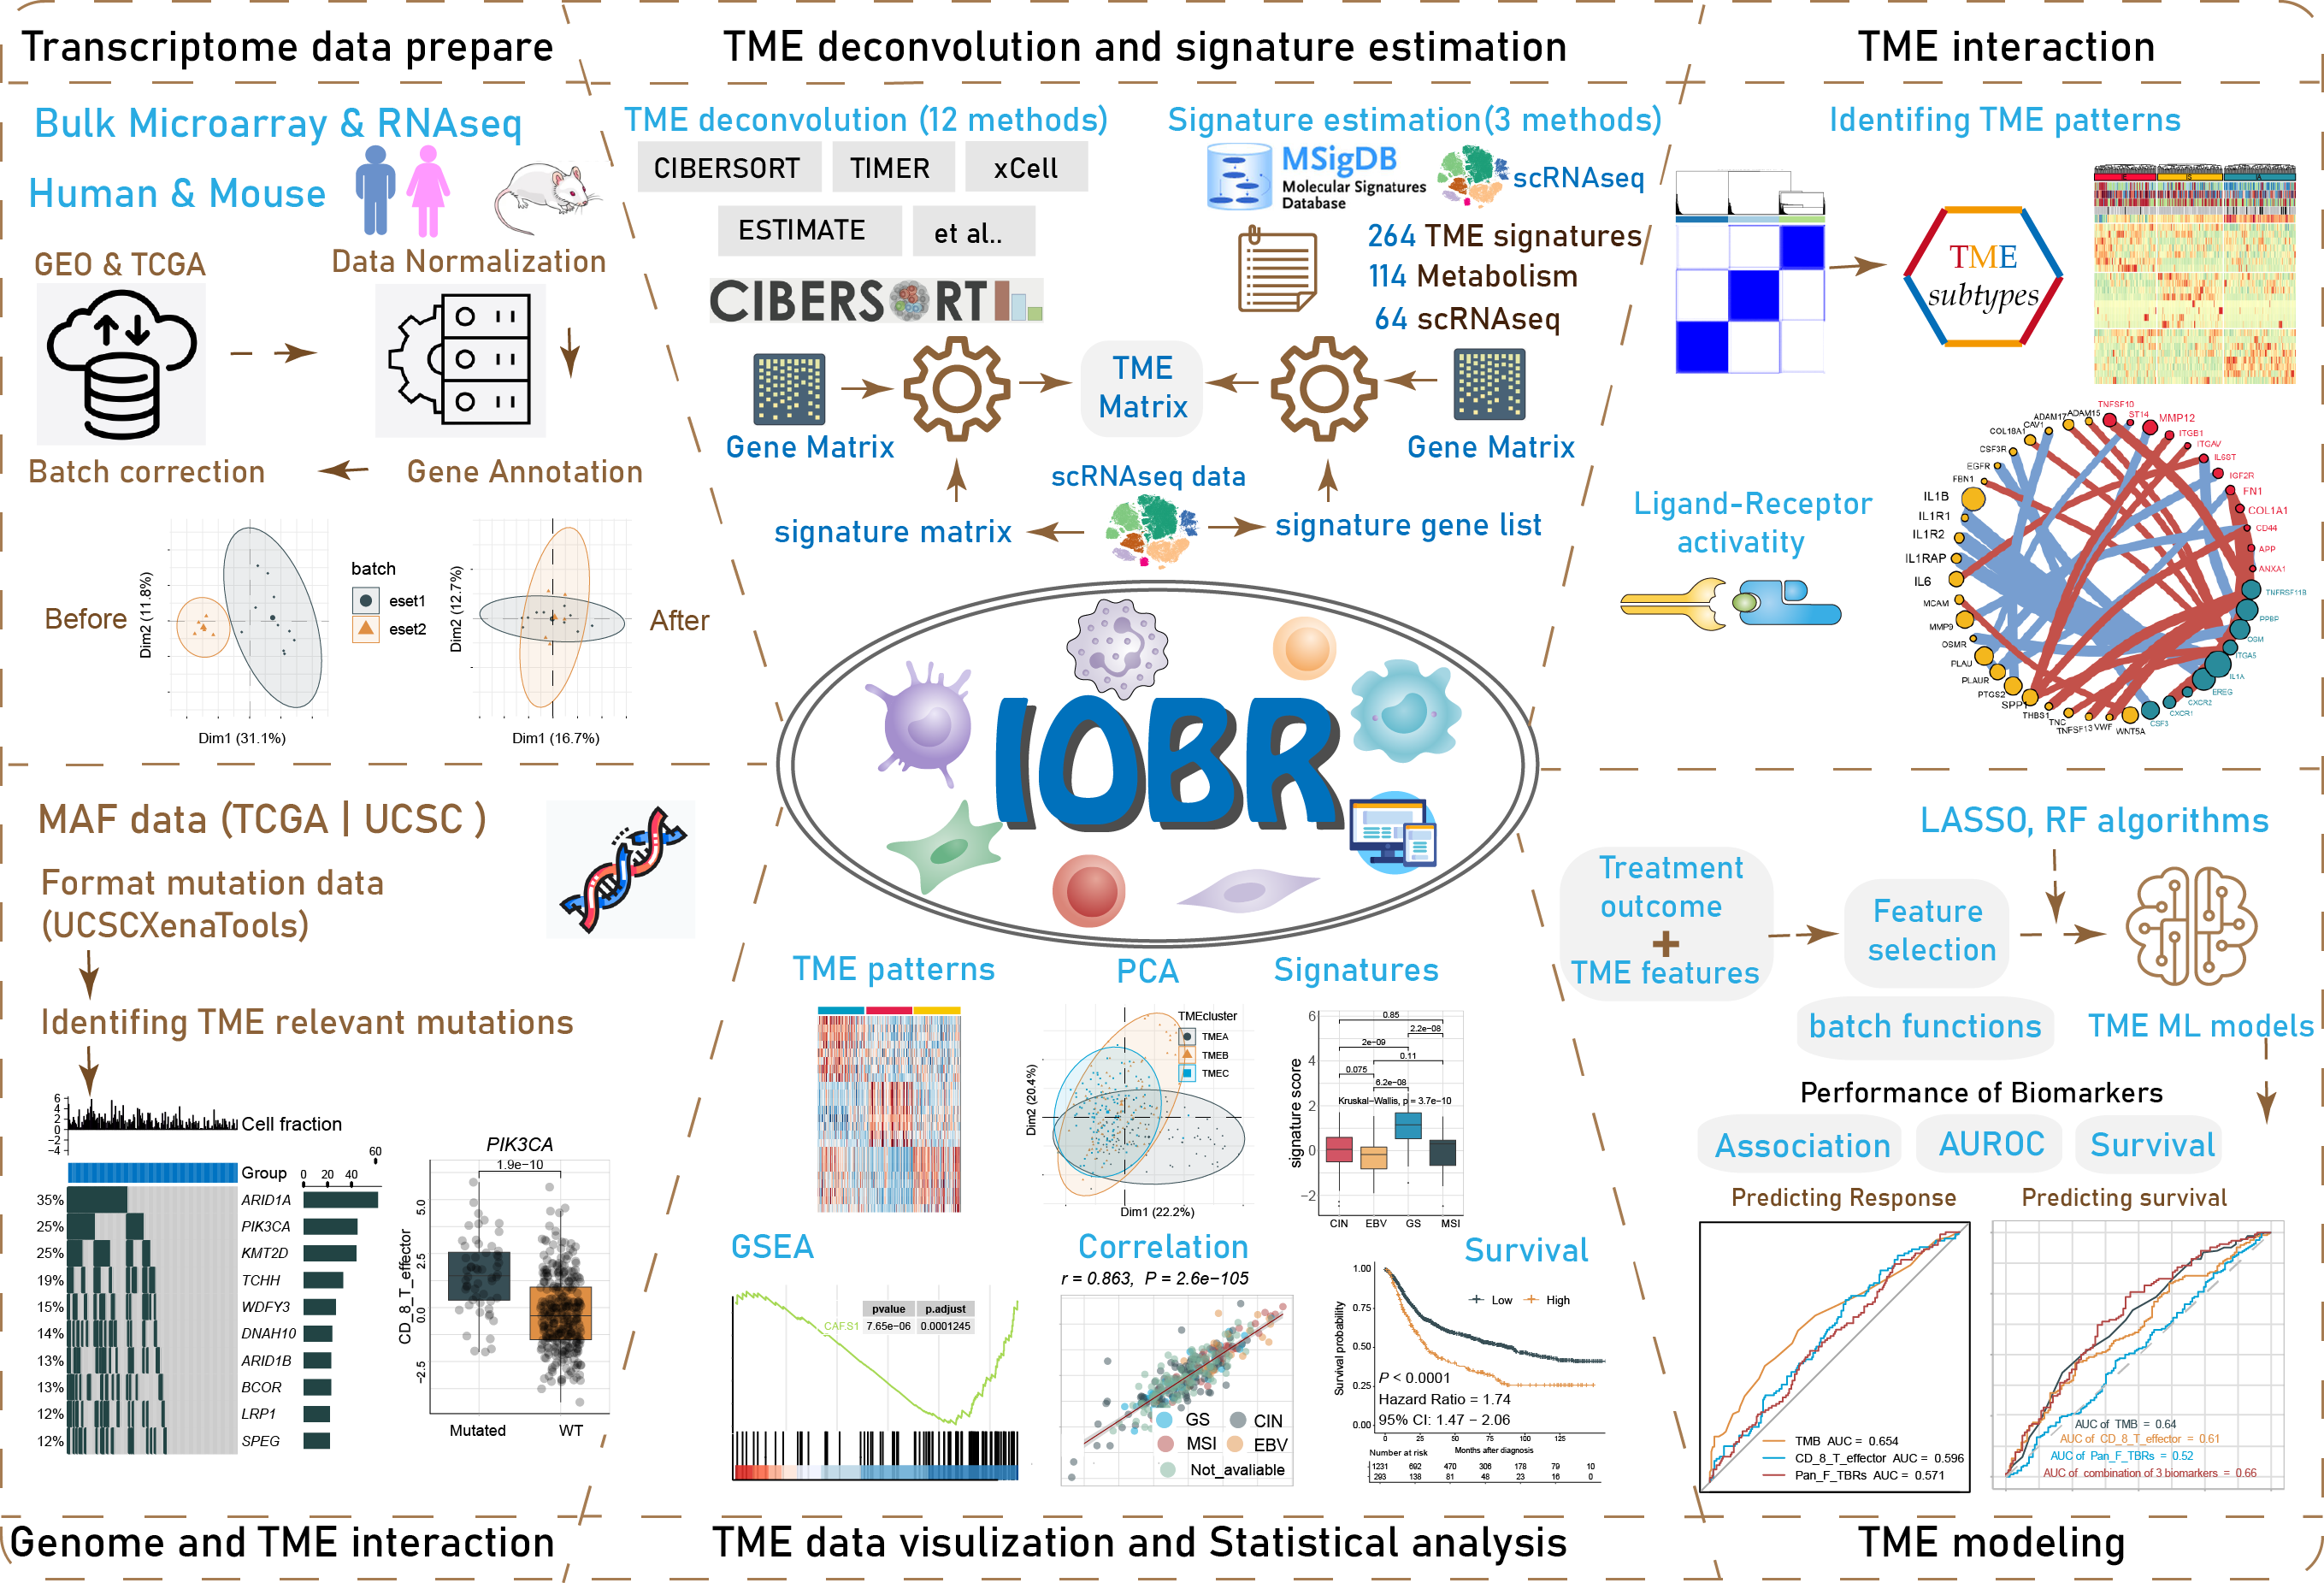
\includegraphics[width=0.95\linewidth]{./fig/IOBR-Workflow} 

}

\caption{The workflow of IOBR}\label{fig:unnamed-chunk-1}
\end{figure}

\hypertarget{introduction-1}{%
\section{Introduction}\label{introduction-1}}

IOBR is design for \href{https://github.com/IOBR/IOBR}{Immuno-Oncology Biological Research}.
Recent advance in next-generation sequencing has triggered the rapidly accumulating publicly available multi-omics data. The application of integrated omics to exploring robust signatures for clinical translation is increasingly highlighted in immuno-oncology but raises computational and biological challenges. This vignette aims to demonstrate how to utilize the package named IOBR to perform multi-omics immuno-oncology biological research to decode tumor microenvironment and signatures for clinical translation.

This R package integrates 8 published methodologies for decoding tumor microenvironment (TME) contexture: \texttt{CIBERSORT}, \texttt{TIMER}, \texttt{xCell}, \texttt{MCPcounter}, \texttt{ESITMATE}, \texttt{EPIC}, \texttt{IPS}, \texttt{quanTIseq}. Moreover, 255 published signature gene sets were collected by IOBR, involving tumor microenvironment, tumor metabolism, m6A, exosomes, microsatellite instability, and tertiary lymphoid structure. Run the function \texttt{signature\_collection\_citation} to obtain the source papers, and the function \texttt{signature\_collection} returns the detail signature genes of all given signatures. Subsequently, IOBR adopts three computational methods to calculate the signature score, comprising \texttt{PCA}, \texttt{z-score}, and \texttt{ssGSEA}. To note, IOBR collected and employed multiple approaches for variable transition, visualization, batch survival analysis, feature selection, and statistical analysis. Batch analysis and visualization of corresponding results are supported. The details of how IOBR works are described below.

\hypertarget{license}{%
\section{License}\label{license}}

\textbf{IOBR} is released under the GPL v3.0 license. See \href{https://github.com/IOBR/IOBR/blob/master/LICENSE}{LICENSE} for details. The code contained in this book is simultaneously available under the \href{https://www.gnu.org/licenses/why-not-lgpl.html}{GPL license}; this means that you are free to use it in your packages, as long as you cite the source. The online version of this book is licensed under the \href{https://creativecommons.org/licenses/by-nc-sa/4.0/}{Creative Commons Attribution-NonCommercial-ShareAlike 4.0 International License.}

\hypertarget{publishment}{%
\section{Publishment}\label{publishment}}

Zeng D, Ye Z, Shen R, Yu G, Wu J, Xiong Y,\ldots, Liao W (2021) \textbf{IOBR}: Multi-Omics Immuno-Oncology Biological Research to Decode Tumor Microenvironment and Signatures. \emph{Frontiers in Immunology}. 12:687975. \href{https://www.frontiersin.org/articles/10.3389/fimmu.2021.687975/full}{doi: 10.3389/fimmu.2021.687975}

\hypertarget{reporting-bugs}{%
\section{Reporting bugs}\label{reporting-bugs}}

Please report bugs to the \href{https://github.com/IOBR/IOBR/issues}{Github issues page}

E-mail any questions to \href{mailto:dongqiangzeng0808@gmail.com}{\nolinkurl{dongqiangzeng0808@gmail.com}}

\hypertarget{how-to-install-iobr}{%
\chapter{\texorpdfstring{\textbf{How to install IOBR}}{How to install IOBR}}\label{how-to-install-iobr}}

\hypertarget{installing-dependency-packages}{%
\section{Installing Dependency Packages}\label{installing-dependency-packages}}

It is essential that you have R 3.6.3 or above already installed on your computer or server. IOBR is a pipeline that utilizes many other R packages that are currently available from CRAN, Bioconductor and GitHub.

\begin{Shaded}
\begin{Highlighting}[]
\ControlFlowTok{if}\NormalTok{ (}\SpecialCharTok{!}\FunctionTok{requireNamespace}\NormalTok{(}\StringTok{"BiocManager"}\NormalTok{, }\AttributeTok{quietly =} \ConstantTok{TRUE}\NormalTok{)) }\FunctionTok{install.packages}\NormalTok{(}\StringTok{"BiocManager"}\NormalTok{)}
\NormalTok{depens}\OtherTok{\textless{}{-}}\FunctionTok{c}\NormalTok{(}\StringTok{\textquotesingle{}tibble\textquotesingle{}}\NormalTok{, }\StringTok{\textquotesingle{}survival\textquotesingle{}}\NormalTok{, }\StringTok{\textquotesingle{}survminer\textquotesingle{}}\NormalTok{, }\StringTok{\textquotesingle{}limma\textquotesingle{}}\NormalTok{, }\StringTok{"DESeq2"}\NormalTok{,}\StringTok{"devtools"}\NormalTok{, }\StringTok{\textquotesingle{}limSolve\textquotesingle{}}\NormalTok{, }\StringTok{\textquotesingle{}GSVA\textquotesingle{}}\NormalTok{, }\StringTok{\textquotesingle{}e1071\textquotesingle{}}\NormalTok{, }\StringTok{\textquotesingle{}preprocessCore\textquotesingle{}}\NormalTok{, }
          \StringTok{"devtools"}\NormalTok{, }\StringTok{"tidyHeatmap"}\NormalTok{, }\StringTok{"caret"}\NormalTok{, }\StringTok{"glmnet"}\NormalTok{, }\StringTok{"ppcor"}\NormalTok{,  }\StringTok{"timeROC"}\NormalTok{, }\StringTok{"pracma"}\NormalTok{, }\StringTok{"factoextra"}\NormalTok{, }
          \StringTok{"FactoMineR"}\NormalTok{, }\StringTok{"WGCNA"}\NormalTok{, }\StringTok{"patchwork"}\NormalTok{, }\StringTok{\textquotesingle{}ggplot2\textquotesingle{}}\NormalTok{, }\StringTok{"biomaRt"}\NormalTok{, }\StringTok{\textquotesingle{}ggpubr\textquotesingle{}}\NormalTok{)}
\ControlFlowTok{for}\NormalTok{(i }\ControlFlowTok{in} \DecValTok{1}\SpecialCharTok{:}\FunctionTok{length}\NormalTok{(depens))\{}
\NormalTok{  depen}\OtherTok{\textless{}{-}}\NormalTok{depens[i]}
  \ControlFlowTok{if}\NormalTok{ (}\SpecialCharTok{!}\FunctionTok{requireNamespace}\NormalTok{(depen, }\AttributeTok{quietly =} \ConstantTok{TRUE}\NormalTok{))  BiocManager}\SpecialCharTok{::}\FunctionTok{install}\NormalTok{(depen,}\AttributeTok{update =} \ConstantTok{FALSE}\NormalTok{)}
\NormalTok{\}}
\end{Highlighting}
\end{Shaded}

\hypertarget{install-iobr-package}{%
\section{Install IOBR package}\label{install-iobr-package}}

When the dependent environments are built, users are able to install IOBR from github by typing the following code into your R session:

\begin{Shaded}
\begin{Highlighting}[]
\ControlFlowTok{if}\NormalTok{ (}\SpecialCharTok{!}\FunctionTok{requireNamespace}\NormalTok{(}\StringTok{"IOBR"}\NormalTok{, }\AttributeTok{quietly =} \ConstantTok{TRUE}\NormalTok{))  devtools}\SpecialCharTok{::}\FunctionTok{install\_github}\NormalTok{(}\StringTok{"IOBR/IOBR"}\NormalTok{)}
\end{Highlighting}
\end{Shaded}

\begin{verbatim}
## Warning: package 'tidyHeatmap' was built under R version 4.2.3
\end{verbatim}

\begin{Shaded}
\begin{Highlighting}[]
\FunctionTok{library}\NormalTok{(IOBR)}
\end{Highlighting}
\end{Shaded}

\begin{verbatim}
## Warning: package 'tibble' was built under R version 4.2.3
\end{verbatim}

\begin{verbatim}
## Warning: package 'dplyr' was built under R version 4.2.3
\end{verbatim}

\begin{verbatim}
## Warning: package 'ggplot2' was built under R version 4.2.3
\end{verbatim}

\hypertarget{the-main-pipeline-of-iobr}{%
\section{The main pipeline of IOBR}\label{the-main-pipeline-of-iobr}}

\begin{figure}

{\centering 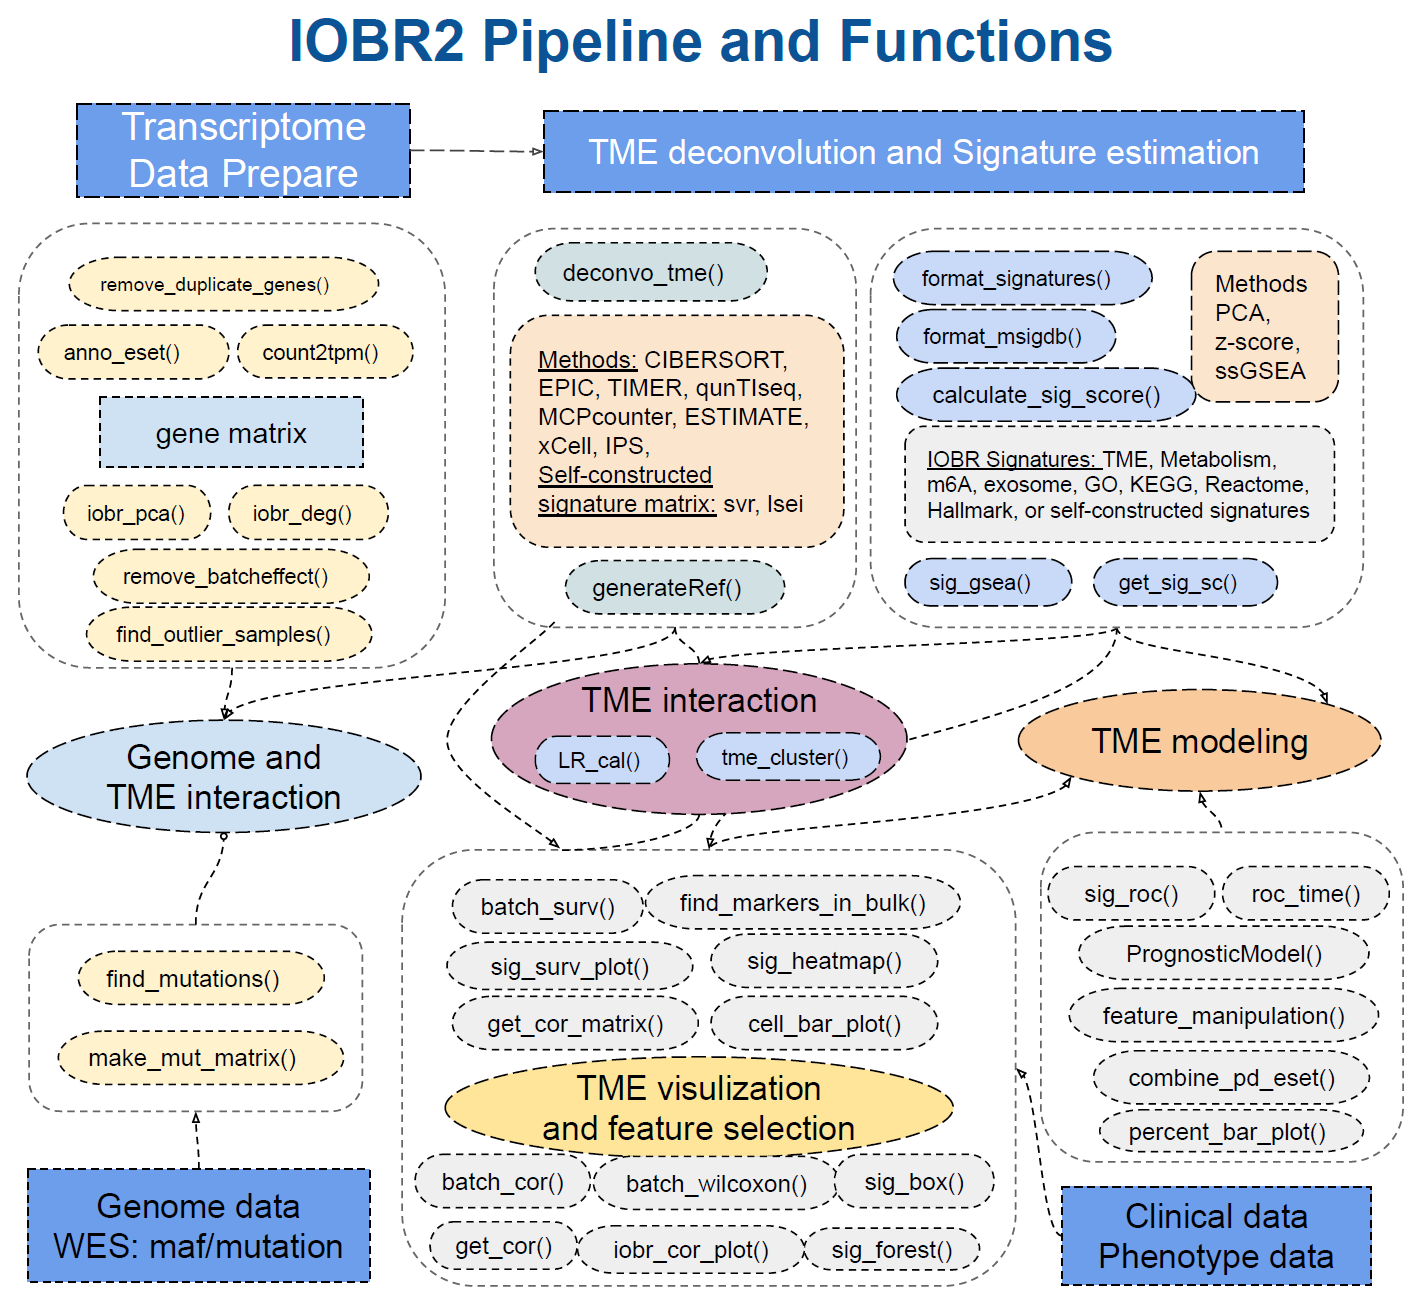
\includegraphics[width=0.95\linewidth]{./fig/IOBR-Package} 

}

\caption{The main pipeline of IOBR}\label{fig:flowchart}
\end{figure}

\hypertarget{main-functions}{%
\section{Main Functions}\label{main-functions}}

\begin{itemize}
\item
  \textbf{Data Preparation: data annotation and transformation}

  \begin{itemize}
  \tightlist
  \item
    \texttt{count2tpm()}: transform count data of RNA sequencing into TPM data.
  \item
    \texttt{anno\_eset()}: annotate the normalized genes expression matrix, including RNAseq and array (Affymetrix or Illumina).
  \item
    \texttt{remove\_duplicate\_genes()}: remove the genes annotated with the duplicated symbol after normalization and retain only the symbol with highest expression level.
  \end{itemize}
\item
  \textbf{TME Deconvolution Module: integrate multiple algorithms to decode immune contexture}

  \begin{itemize}
  \tightlist
  \item
    \texttt{deconvo\_tme()}: decode the TME infiltration with different deconvolution methodologies, based on bulk RNAseq, microarray or single cell RNAseq data.
  \item
    \texttt{generateRef()}: generate a novel gene reference matrix for a specific feature such as infiltrating cell, through the SVR and lsei algorithm.
  \end{itemize}
\item
  \textbf{Signature Module: calculate signature scores, estimate phenotype related signatures and corresponding genes, and evaluate signatures generated from single-cell RNA sequencing data }

  \begin{itemize}
  \tightlist
  \item
    \texttt{calculate\_sig\_score()}: estimate the interested signatures enrolled in IOBR R package, which involves TME-associated, tumor-metabolism, and tumor-intrinsic signatures.
  \item
    \texttt{feature\_manipulation()}: manipulate features including the cell fraction and signatures generated from multi-omics data for latter analysis and model construction. Remove missing values, outliers and variables without significant variance.
  \item
    \texttt{format\_signatures()}: generate the object of \texttt{calculate\_sig\_score()}function, by inputting a data frame with signatures as column names of corresponding gene sets, and return a list contain the signature information for calculating multiple signature scores.
  \item
    \texttt{format\_msigdb()}: transform the signature gene sets data with gmt format, which is not included in the signature collection and might be downloaded in the MSgiDB website, into the object of \texttt{calculate\_sig\_score()}function.
  \end{itemize}
\item
  \textbf{Batch Analysis and Visualization: batch survival analysis and batch correlation analysis and other batch statistical analyses }

  \begin{itemize}
  \tightlist
  \item
    \texttt{batch\_surv}: batch survival analysis of multiple continuous variables including varied signature scores.
  \item
    \texttt{subgroup\_survival}: batch survival analysis of multiple categorized variables with different number of subgroups.
  \item
    \texttt{batch\_cor()}: batch analysis of correlation between two continuous variables using Pearson correlation coefficient or Spearman's rank correlation coefficient .
  \item
    \texttt{batch\_wilcoxon()}: conduct batch wilcoxon analyses of binary variables.
  \item
    \texttt{batch\_pcc()}: batch analyses of Partial Correlation coefficient(PCC) between continuous variables and minimize the interference derived from confounding factors.
  \item
    \texttt{iobr\_cor\_plot()}: visualization of batch correlation analysis of signatures from `sig\_group'. Visualize the correlation between signature or phenotype with expression of gene sets in target signature is also supported.
  \item
    \texttt{cell\_bar\_plot()}: batch visualization of TME cell fraction, supporting input of deconvolution results from `CIBERSORT', `EPIC' and `quanTIseq' methodologies to further compare the TME cell distributions within one sample or among different samples.
  \end{itemize}
\item
  \textbf{Signature Associated Mutation Module: identify and analyze mutations relevant to targeted signatures}

  \begin{itemize}
  \tightlist
  \item
    \texttt{make\_mut\_matrix()}: transform the mutation data with MAF format(contain the columns of gene ID and the corresponding gene alterations which including SNP, indel and frameshift) into a mutation matrix in a suitable manner for further investigating signature relevant mutations.
  \item
    \texttt{find\_mutations()}: identify mutations associated with a distinct phenotype or signature.
  \end{itemize}
\item
  \textbf{Model Construction Module: feature selection and fast model construct to predict clinical phenotype}

  \begin{itemize}
  \tightlist
  \item
    \texttt{BinomialModel()}: select features and construct a model to predict a binary phenotype.
  \item
    \texttt{PrognosticMode()}: select features and construct a model to predict clinical survival outcome.
  \end{itemize}
\end{itemize}

\hypertarget{rna-data-preprocessing}{%
\chapter{\texorpdfstring{\textbf{RNA Data preprocessing}}{RNA Data preprocessing}}\label{rna-data-preprocessing}}

\hypertarget{loading-packages}{%
\section{Loading packages}\label{loading-packages}}

Load the IOBR package in your R session after the installation is complete:

\begin{Shaded}
\begin{Highlighting}[]
\FunctionTok{library}\NormalTok{(IOBR)}
\FunctionTok{library}\NormalTok{(tidyverse)}
\FunctionTok{library}\NormalTok{(clusterProfiler)}
\end{Highlighting}
\end{Shaded}

\hypertarget{downloading-data-for-example}{%
\section{Downloading data for example}\label{downloading-data-for-example}}

Obtaining data set from GEO \href{https://pubmed.ncbi.nlm.nih.gov/25894828/}{Gastric cancer: GSE62254} using \texttt{GEOquery} R package.

\begin{Shaded}
\begin{Highlighting}[]
\ControlFlowTok{if}\NormalTok{ (}\SpecialCharTok{!}\FunctionTok{requireNamespace}\NormalTok{(}\StringTok{"GEOquery"}\NormalTok{, }\AttributeTok{quietly =} \ConstantTok{TRUE}\NormalTok{))  BiocManager}\SpecialCharTok{::}\FunctionTok{install}\NormalTok{(}\StringTok{"GEOquery"}\NormalTok{)}
\FunctionTok{library}\NormalTok{(}\StringTok{"GEOquery"}\NormalTok{)}
\CommentTok{\# }\AlertTok{NOTE}\CommentTok{: This process may take a few minutes which depends on the internet connection speed. Please wait for its completion.}
\NormalTok{eset\_geo}\OtherTok{\textless{}{-}}\FunctionTok{getGEO}\NormalTok{(}\AttributeTok{GEO     =} \StringTok{"GSE62254"}\NormalTok{, }\AttributeTok{getGPL  =}\NormalTok{ F, }\AttributeTok{destdir =} \StringTok{"./"}\NormalTok{)}
\NormalTok{eset    }\OtherTok{\textless{}{-}}\NormalTok{eset\_geo[[}\DecValTok{1}\NormalTok{]]}
\NormalTok{eset    }\OtherTok{\textless{}{-}}\FunctionTok{exprs}\NormalTok{(eset)}
\NormalTok{eset[}\DecValTok{1}\SpecialCharTok{:}\DecValTok{5}\NormalTok{,}\DecValTok{1}\SpecialCharTok{:}\DecValTok{5}\NormalTok{]}
\end{Highlighting}
\end{Shaded}

\begin{verbatim}
##           GSM1523727 GSM1523728 GSM1523729 GSM1523744 GSM1523745
## 1007_s_at  3.2176645  3.0624323  3.0279131   2.921683  2.8456013
## 1053_at    2.4050109  2.4394879  2.2442708   2.345916  2.4328582
## 117_at     1.4933412  1.8067380  1.5959665   1.839822  1.8326058
## 121_at     2.1965561  2.2812181  2.1865556   2.258599  2.1874363
## 1255_g_at  0.8698382  0.9502466  0.8125414   1.012860  0.9441993
\end{verbatim}

\hypertarget{gene-annotation}{%
\section{Gene Annotation}\label{gene-annotation}}

Annotation of genes in the expression matrix and removal of duplicate genes.

\begin{Shaded}
\begin{Highlighting}[]
\CommentTok{\# Load the annotation file \textasciigrave{}anno\_hug133plus2\textasciigrave{} in IOBR.}
\FunctionTok{head}\NormalTok{(anno\_hug133plus2)}
\end{Highlighting}
\end{Shaded}

\begin{verbatim}
## # A tibble: 6 x 2
##   probe_id  symbol 
##   <fct>     <fct>  
## 1 1007_s_at MIR4640
## 2 1053_at   RFC2   
## 3 117_at    HSPA6  
## 4 121_at    PAX8   
## 5 1255_g_at GUCA1A 
## 6 1294_at   MIR5193
\end{verbatim}

\begin{Shaded}
\begin{Highlighting}[]
\CommentTok{\# Load the annotation file \textasciigrave{}anno\_grch38\textasciigrave{} in IOBR.}
\FunctionTok{head}\NormalTok{(anno\_grch38)}
\end{Highlighting}
\end{Shaded}

\begin{verbatim}
##                id eff_length        gc entrez   symbol chr     start       end
## 1 ENSG00000000003       4536 0.3992504   7105   TSPAN6   X 100627109 100639991
## 2 ENSG00000000005       1476 0.4241192  64102     TNMD   X 100584802 100599885
## 3 ENSG00000000419       9276 0.4252911   8813     DPM1  20  50934867  50958555
## 4 ENSG00000000457       6883 0.4117391  57147    SCYL3   1 169849631 169894267
## 5 ENSG00000000460       5970 0.4298157  55732 C1orf112   1 169662007 169854080
## 6 ENSG00000000938       3382 0.5644589   2268      FGR   1  27612064  27635277
##   strand        biotype
## 1     -1 protein_coding
## 2      1 protein_coding
## 3     -1 protein_coding
## 4     -1 protein_coding
## 5      1 protein_coding
## 6     -1 protein_coding
##                                                                                                  description
## 1                                                          tetraspanin 6 [Source:HGNC Symbol;Acc:HGNC:11858]
## 2                                                            tenomodulin [Source:HGNC Symbol;Acc:HGNC:17757]
## 3 dolichyl-phosphate mannosyltransferase polypeptide 1, catalytic subunit [Source:HGNC Symbol;Acc:HGNC:3005]
## 4                                               SCY1-like, kinase-like 3 [Source:HGNC Symbol;Acc:HGNC:19285]
## 5                                    chromosome 1 open reading frame 112 [Source:HGNC Symbol;Acc:HGNC:25565]
## 6                          FGR proto-oncogene, Src family tyrosine kinase [Source:HGNC Symbol;Acc:HGNC:3697]
\end{verbatim}

\begin{Shaded}
\begin{Highlighting}[]
\CommentTok{\# Load the annotation file \textasciigrave{}anno\_gc\_vm32\textasciigrave{} in IOBR for mouse RNAseq data}
\FunctionTok{head}\NormalTok{(anno\_gc\_vm32)}
\end{Highlighting}
\end{Shaded}

\begin{verbatim}
##                   id eff_length        gc symbol      mgi_id      gene_type
## 1 ENSMUSG00000000001       3262 0.4350092  Gnai3   MGI:95773 protein_coding
## 2 ENSMUSG00000000003        902 0.3481153   Pbsn MGI:1860484 protein_coding
## 3 ENSMUSG00000000028       3506 0.4962921  Cdc45 MGI:1338073 protein_coding
## 4 ENSMUSG00000000031       2625 0.5588571    H19   MGI:95891         lncRNA
## 5 ENSMUSG00000000037       6397 0.4377052  Scml2 MGI:1340042 protein_coding
## 6 ENSMUSG00000000049       1594 0.5050188   Apoh   MGI:88058 protein_coding
##       start       end transcript_id  ont
## 1 108014596 108053462          <NA> <NA>
## 2  76881507  76897229          <NA> <NA>
## 3  18599197  18630737          <NA> <NA>
## 4 142129262 142131886          <NA> <NA>
## 5 159865521 160041209          <NA> <NA>
## 6 108234180 108305222          <NA> <NA>
\end{verbatim}

\hypertarget{for-array-data-hgu133plus-2-affaymetrix}{%
\subsection{For Array data: HGU133PLUS-2 (Affaymetrix)}\label{for-array-data-hgu133plus-2-affaymetrix}}

\begin{Shaded}
\begin{Highlighting}[]
\CommentTok{\# Conduct gene annotation using \textasciigrave{}anno\_hug133plus2\textasciigrave{} file; If identical gene symbols exists, these genes would be ordered by the mean expression levels. The gene symbol with highest mean expression level is selected and remove others. }

\NormalTok{eset}\OtherTok{\textless{}{-}}\FunctionTok{anno\_eset}\NormalTok{(}\AttributeTok{eset       =}\NormalTok{ eset,}
                \AttributeTok{annotation =}\NormalTok{ anno\_hug133plus2,}
                \AttributeTok{symbol     =} \StringTok{"symbol"}\NormalTok{,}
                \AttributeTok{probe      =} \StringTok{"probe\_id"}\NormalTok{,}
                \AttributeTok{method     =} \StringTok{"mean"}\NormalTok{)}
\NormalTok{eset[}\DecValTok{1}\SpecialCharTok{:}\DecValTok{5}\NormalTok{, }\DecValTok{1}\SpecialCharTok{:}\DecValTok{3}\NormalTok{]}
\end{Highlighting}
\end{Shaded}

\begin{verbatim}
##              GSM1523727 GSM1523728 GSM1523729
## SH3KBP1        4.327974   4.316195   4.351425
## RPL41          4.246149   4.246808   4.257940
## EEF1A1         4.293762   4.291038   4.262199
## COX2           4.250288   4.283714   4.270508
## LOC101928826   4.219303   4.219670   4.213252
\end{verbatim}

\hypertarget{for-rnaseq-data}{%
\subsection{For RNAseq data}\label{for-rnaseq-data}}

Download RNAseq data using UCSCXenaTools

Transform gene expression matrix into TPM format, and conduct subsequent annotation.

\hypertarget{identifying-outlier-samples}{%
\section{Identifying outlier samples}\label{identifying-outlier-samples}}

Take ACRG microarray data for example

\begin{Shaded}
\begin{Highlighting}[]
\CommentTok{\# source("E:/18{-}Github/Organization/IOBR/R/find\_outlier\_samples.R")}
\NormalTok{res }\OtherTok{\textless{}{-}} \FunctionTok{find\_outlier\_samples}\NormalTok{(}\AttributeTok{eset =}\NormalTok{ eset, }\AttributeTok{project =} \StringTok{"ACRG"}\NormalTok{, }\AttributeTok{show\_plot =} \ConstantTok{TRUE}\NormalTok{)}
\end{Highlighting}
\end{Shaded}

\begin{center}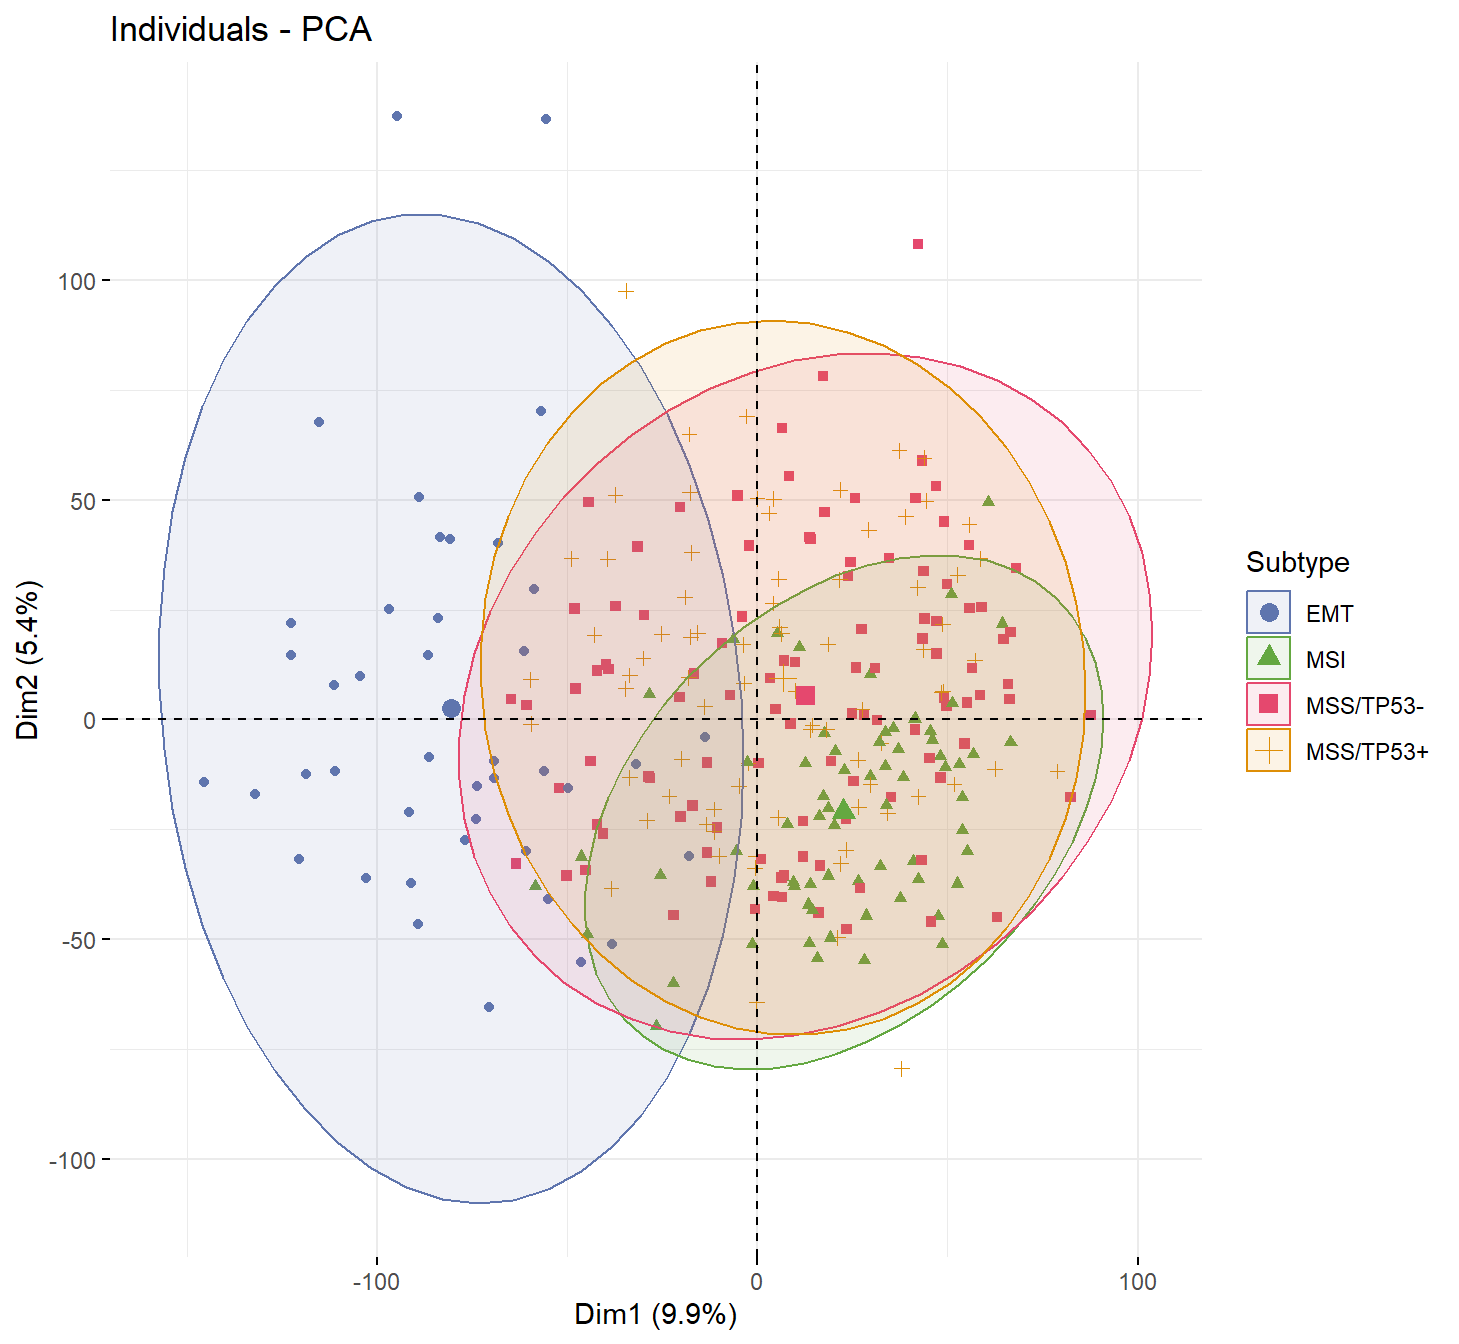
\includegraphics{data-preprocessing_files/figure-latex/unnamed-chunk-9-1} \end{center}

\begin{verbatim}
## [1] "GSM1523817" "GSM1523858" "GSM1523984" "GSM1523988" "GSM1524030"
\end{verbatim}

\begin{Shaded}
\begin{Highlighting}[]
\NormalTok{eset1 }\OtherTok{\textless{}{-}}\NormalTok{ eset[, }\SpecialCharTok{!}\FunctionTok{colnames}\NormalTok{(eset)}\SpecialCharTok{\%in\%}\NormalTok{res]}
\end{Highlighting}
\end{Shaded}

\hypertarget{pca-analysis-of-molecular-subtypes}{%
\section{PCA analysis of molecular subtypes}\label{pca-analysis-of-molecular-subtypes}}

\begin{Shaded}
\begin{Highlighting}[]
\FunctionTok{data}\NormalTok{(}\StringTok{"pdata\_acrg"}\NormalTok{)}
\NormalTok{res}\OtherTok{\textless{}{-}} \FunctionTok{iobr\_pca}\NormalTok{(}\AttributeTok{data       =}\NormalTok{ eset1,}
              \AttributeTok{is.matrix   =} \ConstantTok{TRUE}\NormalTok{,}
              \AttributeTok{scale       =} \ConstantTok{TRUE}\NormalTok{,}
              \AttributeTok{is.log      =} \ConstantTok{FALSE}\NormalTok{,}
              \AttributeTok{pdata       =}\NormalTok{ pdata\_acrg, }
              \AttributeTok{id\_pdata    =} \StringTok{"ID"}\NormalTok{, }
              \AttributeTok{group       =} \StringTok{"Subtype"}\NormalTok{,}
              \AttributeTok{geom.ind    =} \StringTok{"point"}\NormalTok{, }
              \AttributeTok{cols        =} \StringTok{"normal"}\NormalTok{,}
              \AttributeTok{palette     =} \StringTok{"jama"}\NormalTok{, }
              \AttributeTok{repel       =} \ConstantTok{FALSE}\NormalTok{,}
              \AttributeTok{ncp         =} \DecValTok{5}\NormalTok{,}
              \AttributeTok{axes        =} \FunctionTok{c}\NormalTok{(}\DecValTok{1}\NormalTok{, }\DecValTok{2}\NormalTok{),}
              \AttributeTok{addEllipses =} \ConstantTok{TRUE}\NormalTok{)}
\end{Highlighting}
\end{Shaded}

\begin{verbatim}
## 
##       CIN       EBV       EMT        GS       MSI MSS/TP53- MSS/TP53+ 
##         0         0        42         0        68       106        79 
## [1] ">>-- colors for PCA: #5f75ae" ">>-- colors for PCA: #64a841"
## [3] ">>-- colors for PCA: #e5486e" ">>-- colors for PCA: #de8e06"
\end{verbatim}

\begin{Shaded}
\begin{Highlighting}[]
\NormalTok{res}
\end{Highlighting}
\end{Shaded}

\begin{center}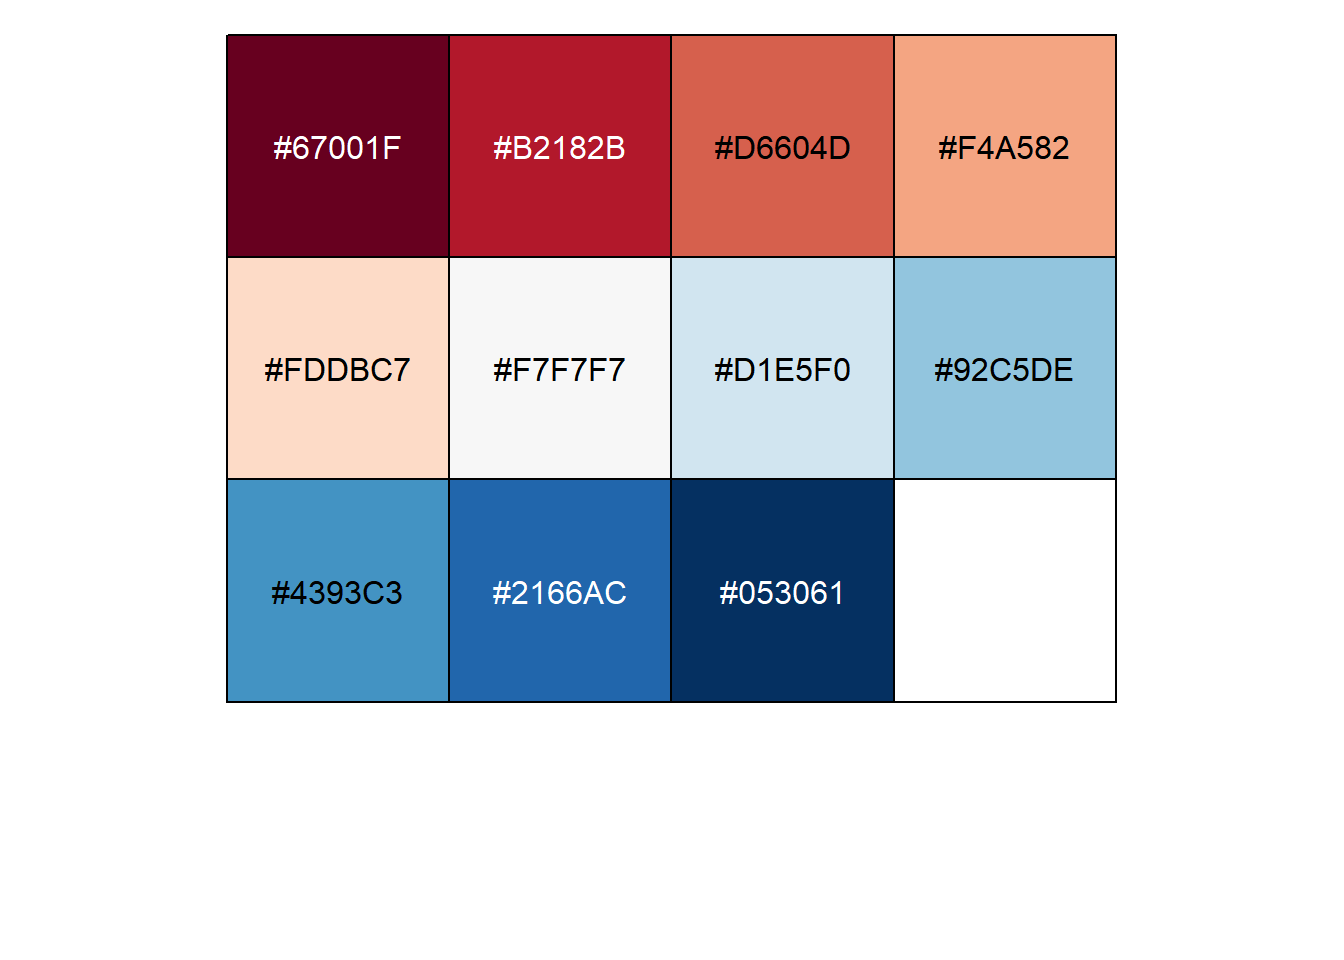
\includegraphics{data-preprocessing_files/figure-latex/unnamed-chunk-10-1} \end{center}

\hypertarget{batch-effect-correction}{%
\section{Batch effect correction}\label{batch-effect-correction}}

Obtaining another data set from GEO \href{https://www.ncbi.nlm.nih.gov/pubmed/24935174/}{Gastric cancer: GSE57303} using \texttt{GEOquery} R package.

\begin{Shaded}
\begin{Highlighting}[]
\CommentTok{\# }\AlertTok{NOTE}\CommentTok{: This process may take a few minutes which depends on the internet connection speed. Please wait for its completion.}
\NormalTok{eset\_geo}\OtherTok{\textless{}{-}}\FunctionTok{getGEO}\NormalTok{(}\AttributeTok{GEO     =} \StringTok{"GSE57303"}\NormalTok{, }\AttributeTok{getGPL  =}\NormalTok{ F, }\AttributeTok{destdir =} \StringTok{"./"}\NormalTok{)}
\NormalTok{eset2    }\OtherTok{\textless{}{-}}\NormalTok{eset\_geo[[}\DecValTok{1}\NormalTok{]]}
\NormalTok{eset2    }\OtherTok{\textless{}{-}}\FunctionTok{exprs}\NormalTok{(eset2)}
\NormalTok{eset2[}\DecValTok{1}\SpecialCharTok{:}\DecValTok{5}\NormalTok{,}\DecValTok{1}\SpecialCharTok{:}\DecValTok{5}\NormalTok{]}
\end{Highlighting}
\end{Shaded}

\begin{verbatim}
##           GSM1379261 GSM1379262 GSM1379263 GSM1379264 GSM1379265
## 1007_s_at    8.34746    9.67994    8.62643    8.59301    8.63046
## 1053_at      5.07972    4.46377    5.29685    5.78983    4.33359
## 117_at       5.65558    4.48732    4.21615    5.47984    5.20816
## 121_at       5.95123    7.09056    6.19903    5.89872    5.91323
## 1255_g_at    1.66923    1.98758    1.73083    1.56687    1.63332
\end{verbatim}

Annotation of genes in the expression matrix and removal of duplicate genes.

\begin{Shaded}
\begin{Highlighting}[]
\NormalTok{eset2}\OtherTok{\textless{}{-}}\FunctionTok{anno\_eset}\NormalTok{(}\AttributeTok{eset       =}\NormalTok{ eset2,}
                 \AttributeTok{annotation =}\NormalTok{ anno\_hug133plus2,}
                 \AttributeTok{symbol     =} \StringTok{"symbol"}\NormalTok{,}
                 \AttributeTok{probe      =} \StringTok{"probe\_id"}\NormalTok{,}
                 \AttributeTok{method     =} \StringTok{"mean"}\NormalTok{)}
\NormalTok{eset2[}\DecValTok{1}\SpecialCharTok{:}\DecValTok{5}\NormalTok{, }\DecValTok{1}\SpecialCharTok{:}\DecValTok{5}\NormalTok{]}
\end{Highlighting}
\end{Shaded}

\begin{verbatim}
##         GSM1379261 GSM1379262 GSM1379263 GSM1379264 GSM1379265
## ND4        13.1695    13.1804    13.0600    12.4544    13.0457
## ATP6       13.1433    13.0814    13.0502    12.4831    13.1168
## SH3KBP1    12.9390    13.1620    12.9773    12.8745    13.1169
## COX2       13.0184    13.0489    12.8621    12.7489    12.9732
## RPL41      13.0201    12.6034    12.7929    13.0153    12.9404
\end{verbatim}

\begin{Shaded}
\begin{Highlighting}[]
\NormalTok{eset\_com }\OtherTok{\textless{}{-}} \FunctionTok{remove\_batcheffect}\NormalTok{( }\AttributeTok{eset1       =}\NormalTok{ eset1,  }
                                \AttributeTok{eset2       =}\NormalTok{ eset2,   }
                                \AttributeTok{eset3       =} \ConstantTok{NULL}\NormalTok{,}
                                \AttributeTok{id\_type     =} \StringTok{"symbol"}\NormalTok{,}
                                \AttributeTok{data\_type   =} \StringTok{"array"}\NormalTok{, }
                                \AttributeTok{cols        =} \StringTok{"normal"}\NormalTok{, }
                                \AttributeTok{palette     =} \StringTok{"jama"}\NormalTok{, }
                                \AttributeTok{log2        =} \ConstantTok{TRUE}\NormalTok{, }
                                \AttributeTok{check\_eset  =} \ConstantTok{TRUE}\NormalTok{,}
                                \AttributeTok{adjust\_eset =} \ConstantTok{TRUE}\NormalTok{,}
                                \AttributeTok{repel       =} \ConstantTok{FALSE}\NormalTok{,}
                                \AttributeTok{path        =} \StringTok{"result"}\NormalTok{)}
\end{Highlighting}
\end{Shaded}

\begin{verbatim}
## 
## eset1 eset2 
##   295    70 
## [1] ">>-- colors for PCA: #5f75ae" ">>-- colors for PCA: #64a841"
## 
## eset1 eset2 
##   295    70 
## [1] ">>-- colors for PCA: #5f75ae" ">>-- colors for PCA: #64a841"
\end{verbatim}

\begin{center}\includegraphics{data-preprocessing_files/figure-latex/unnamed-chunk-13-1} \end{center}

\begin{Shaded}
\begin{Highlighting}[]
\FunctionTok{dim}\NormalTok{(eset\_com)}
\end{Highlighting}
\end{Shaded}

\begin{verbatim}
## [1] 21752   365
\end{verbatim}

待补充-RNAseq的批次校正:count, combat-seq

\hypertarget{references}{%
\section{References}\label{references}}

Yuqing Zhang and others, ComBat-seq: batch effect adjustment for RNA-seq count data, NAR Genomics and Bioinformatics, Volume 2, Issue 3, September 2020, lqaa078, \url{https://doi.org/10.1093/nargab/lqaa078}

Leek, J. T., Johnson, W. E., Parker, H. S., Jaffe, A. E., \& Storey, J. D. (2012). The sva package for removing batch effects and other unwanted variation in high-throughput experiments. Bioinformatics, 28(6), 882-883.

\hypertarget{tumor-ecosystem-analysis}{%
\chapter{\texorpdfstring{\textbf{Tumor ecosystem analysis}}{Tumor ecosystem analysis}}\label{tumor-ecosystem-analysis}}

\hypertarget{loading-packages-1}{%
\section{Loading packages}\label{loading-packages-1}}

\begin{Shaded}
\begin{Highlighting}[]
\FunctionTok{library}\NormalTok{(IOBR)}
\end{Highlighting}
\end{Shaded}

\hypertarget{downloading-data-for-example-1}{%
\section{Downloading data for example}\label{downloading-data-for-example-1}}

Obtaining data set from GEO \href{https://pubmed.ncbi.nlm.nih.gov/25894828/}{Gastric cancer: GSE62254} using \texttt{GEOquery} R package.

\begin{Shaded}
\begin{Highlighting}[]
\ControlFlowTok{if}\NormalTok{ (}\SpecialCharTok{!}\FunctionTok{requireNamespace}\NormalTok{(}\StringTok{"GEOquery"}\NormalTok{, }\AttributeTok{quietly =} \ConstantTok{TRUE}\NormalTok{))  BiocManager}\SpecialCharTok{::}\FunctionTok{install}\NormalTok{(}\StringTok{"GEOquery"}\NormalTok{)}
\FunctionTok{library}\NormalTok{(}\StringTok{"GEOquery"}\NormalTok{)}
\CommentTok{\# }\AlertTok{NOTE}\CommentTok{: This process may take a few minutes which depends on the internet connection speed. Please wait for its completion.}
\NormalTok{eset\_geo}\OtherTok{\textless{}{-}}\FunctionTok{getGEO}\NormalTok{(}\AttributeTok{GEO     =} \StringTok{"GSE62254"}\NormalTok{, }\AttributeTok{getGPL  =}\NormalTok{ F, }\AttributeTok{destdir =} \StringTok{"./"}\NormalTok{)}
\NormalTok{eset    }\OtherTok{\textless{}{-}}\NormalTok{eset\_geo[[}\DecValTok{1}\NormalTok{]]}
\NormalTok{eset    }\OtherTok{\textless{}{-}}\FunctionTok{exprs}\NormalTok{(eset)}
\NormalTok{eset[}\DecValTok{1}\SpecialCharTok{:}\DecValTok{5}\NormalTok{,}\DecValTok{1}\SpecialCharTok{:}\DecValTok{5}\NormalTok{]}
\end{Highlighting}
\end{Shaded}

\begin{verbatim}
##           GSM1523727 GSM1523728 GSM1523729 GSM1523744 GSM1523745
## 1007_s_at  3.2176645  3.0624323  3.0279131   2.921683  2.8456013
## 1053_at    2.4050109  2.4394879  2.2442708   2.345916  2.4328582
## 117_at     1.4933412  1.8067380  1.5959665   1.839822  1.8326058
## 121_at     2.1965561  2.2812181  2.1865556   2.258599  2.1874363
## 1255_g_at  0.8698382  0.9502466  0.8125414   1.012860  0.9441993
\end{verbatim}

\hypertarget{gene-annotation-hgu133plus-2-affaymetrix}{%
\section{Gene Annotation: HGU133PLUS-2 (Affaymetrix)}\label{gene-annotation-hgu133plus-2-affaymetrix}}

\begin{Shaded}
\begin{Highlighting}[]
\CommentTok{\# Conduct gene annotation using \textasciigrave{}anno\_hug133plus2\textasciigrave{} file; If identical gene symbols exists, these genes would be ordered by the mean expression levels. The gene symbol with highest mean expression level is selected and remove others. }

\NormalTok{eset}\OtherTok{\textless{}{-}}\FunctionTok{anno\_eset}\NormalTok{(}\AttributeTok{eset       =}\NormalTok{ eset,}
                \AttributeTok{annotation =}\NormalTok{ anno\_hug133plus2,}
                \AttributeTok{symbol     =} \StringTok{"symbol"}\NormalTok{,}
                \AttributeTok{probe      =} \StringTok{"probe\_id"}\NormalTok{,}
                \AttributeTok{method     =} \StringTok{"mean"}\NormalTok{)}
\NormalTok{eset[}\DecValTok{1}\SpecialCharTok{:}\DecValTok{5}\NormalTok{, }\DecValTok{1}\SpecialCharTok{:}\DecValTok{3}\NormalTok{]}
\end{Highlighting}
\end{Shaded}

\begin{verbatim}
##              GSM1523727 GSM1523728 GSM1523729
## SH3KBP1        4.327974   4.316195   4.351425
## RPL41          4.246149   4.246808   4.257940
## EEF1A1         4.293762   4.291038   4.262199
## COX2           4.250288   4.283714   4.270508
## LOC101928826   4.219303   4.219670   4.213252
\end{verbatim}

\hypertarget{determine-tme-subtype-of-gastric-cancer-using-tmeclassifier}{%
\section{Determine TME subtype of gastric cancer using TMEclassifier}\label{determine-tme-subtype-of-gastric-cancer-using-tmeclassifier}}

加载TME分类器R包\href{https://github.com/LiaoWJLab/TMEclassifier}{TMEclassifier}

\begin{Shaded}
\begin{Highlighting}[]
\FunctionTok{library}\NormalTok{(TMEclassifier)}
\NormalTok{tme }\OtherTok{\textless{}{-}} \FunctionTok{tme\_classifier}\NormalTok{(}\AttributeTok{eset =}\NormalTok{ eset, }\AttributeTok{scale =} \ConstantTok{TRUE}\NormalTok{)}
\end{Highlighting}
\end{Shaded}

\begin{verbatim}
## Step-1: Expression data preprocessing...
## Step-2: TME deconvolution...
## Step-3: Predicting TME phenotypes...
## [09:58:03] WARNING: amalgamation/../src/learner.cc:1040: 
##   If you are loading a serialized model (like pickle in Python, RDS in R) generated by
##   older XGBoost, please export the model by calling `Booster.save_model` from that version
##   first, then load it back in current version. See:
## 
##     https://xgboost.readthedocs.io/en/latest/tutorials/saving_model.html
## 
##   for more details about differences between saving model and serializing.
## 
## [09:58:03] WARNING: amalgamation/../src/learner.cc:749: Found JSON model saved before XGBoost 1.6, please save the model using current version again. The support for old JSON model will be discontinued in XGBoost 2.3.
## >>>--- DONE!
\end{verbatim}

\begin{Shaded}
\begin{Highlighting}[]
\FunctionTok{table}\NormalTok{(tme}\SpecialCharTok{$}\NormalTok{TMEcluster)}
\end{Highlighting}
\end{Shaded}

\begin{verbatim}
## 
##  IA  IE  IS 
## 107  96  97
\end{verbatim}

\begin{Shaded}
\begin{Highlighting}[]
\FunctionTok{head}\NormalTok{(tme)}
\end{Highlighting}
\end{Shaded}

\begin{verbatim}
##           ID          IE         IS         IA TMEcluster
## 1 GSM1523727 0.204623557 0.11212681 0.68324962         IA
## 2 GSM1523728 0.009599504 0.11179146 0.87860903         IA
## 3 GSM1523729 0.852615046 0.11369089 0.03369407         IE
## 4 GSM1523744 0.053842233 0.06994632 0.87621145         IA
## 5 GSM1523745 0.055973019 0.80839488 0.13563209         IS
## 6 GSM1523746 0.545343299 0.37437568 0.08028102         IE
\end{verbatim}

\begin{Shaded}
\begin{Highlighting}[]
\FunctionTok{table}\NormalTok{(tme}\SpecialCharTok{$}\NormalTok{TMEcluster)}
\end{Highlighting}
\end{Shaded}

\begin{verbatim}
## 
##  IA  IE  IS 
## 107  96  97
\end{verbatim}

\begin{Shaded}
\begin{Highlighting}[]
\FunctionTok{head}\NormalTok{(tme)}
\end{Highlighting}
\end{Shaded}

\begin{verbatim}
##           ID          IE         IS         IA TMEcluster
## 1 GSM1523727 0.204623557 0.11212681 0.68324962         IA
## 2 GSM1523728 0.009599504 0.11179146 0.87860903         IA
## 3 GSM1523729 0.852615046 0.11369089 0.03369407         IE
## 4 GSM1523744 0.053842233 0.06994632 0.87621145         IA
## 5 GSM1523745 0.055973019 0.80839488 0.13563209         IS
## 6 GSM1523746 0.545343299 0.37437568 0.08028102         IE
\end{verbatim}

\hypertarget{deg-analysis}{%
\section{DEG analysis}\label{deg-analysis}}

选择IA和IE分型进行差异分析

\begin{Shaded}
\begin{Highlighting}[]
\NormalTok{pdata }\OtherTok{\textless{}{-}}\NormalTok{ tme[}\SpecialCharTok{!}\NormalTok{tme}\SpecialCharTok{$}\NormalTok{TMEcluster}\SpecialCharTok{==}\StringTok{"IS"}\NormalTok{, ]}
\NormalTok{deg  }\OtherTok{\textless{}{-}}   \FunctionTok{iobr\_deg}\NormalTok{(}\AttributeTok{eset         =}\NormalTok{ eset,}
                   \AttributeTok{annoation    =} \ConstantTok{NULL}\NormalTok{,}
                   \AttributeTok{pdata        =}\NormalTok{ pdata,}
                   \AttributeTok{group\_id     =} \StringTok{"TMEcluster"}\NormalTok{,}
                   \AttributeTok{pdata\_id     =} \StringTok{"ID"}\NormalTok{,}
                   \AttributeTok{array        =} \ConstantTok{TRUE}\NormalTok{,}
                   \AttributeTok{method       =} \StringTok{"limma"}\NormalTok{,}
                   \AttributeTok{contrast     =} \FunctionTok{c}\NormalTok{(}\StringTok{"deg\_group"}\NormalTok{,}\StringTok{"IA"}\NormalTok{,}\StringTok{"IE"}\NormalTok{),}
                   \AttributeTok{path         =} \ConstantTok{NULL}\NormalTok{,}
                   \AttributeTok{padj\_cutoff  =} \FloatTok{0.01}\NormalTok{,}
                   \AttributeTok{logfc\_cutoff =} \FloatTok{0.5}\NormalTok{)}
\end{Highlighting}
\end{Shaded}

\begin{verbatim}
## 
## Attaching package: 'limma'
\end{verbatim}

\begin{verbatim}
## The following object is masked from 'package:BiocGenerics':
## 
##     plotMA
\end{verbatim}

\begin{verbatim}
## group1 = IA
\end{verbatim}

\begin{verbatim}
## group2 = IE
\end{verbatim}

\begin{verbatim}
## # A tibble: 6 x 11
##   symbol  log2FoldChange AveExpr     t   pvalue     padj     B sigORnot    label
##   <chr>            <dbl>   <dbl> <dbl>    <dbl>    <dbl> <dbl> <chr>       <chr>
## 1 TMEM100         -0.774    1.84 -13.9 2.47e-31 5.37e-27  60.4 Down_regul~ Both 
## 2 ABCA8           -0.933    1.90 -12.9 3.11e-28 3.38e-24  53.4 Down_regul~ Both 
## 3 HHIP            -0.613    1.73 -12.1 7.62e-26 4.46e-22  48.0 Down_regul~ Both 
## 4 LMNB2            0.287    2.25  12.1 9.28e-26 4.46e-22  47.8 NOT         Sign~
## 5 MCM6             0.211    3.02  12.1 1.02e-25 4.46e-22  47.7 NOT         Sign~
## 6 ADH1B           -0.907    1.86 -12.0 2.27e-25 7.04e-22  47.0 Down_regul~ Both 
## # i 2 more variables: IA <dbl>, IE <dbl>
\end{verbatim}

\hypertarget{gsea-analysis-of-degs}{%
\section{GSEA analysis of DEGs}\label{gsea-analysis-of-degs}}

选择IOBR的signature collection

\begin{Shaded}
\begin{Highlighting}[]
\FunctionTok{head}\NormalTok{(deg)}
\end{Highlighting}
\end{Shaded}

\begin{verbatim}
## # A tibble: 6 x 11
##   symbol  log2FoldChange AveExpr     t   pvalue     padj     B sigORnot    label
##   <chr>            <dbl>   <dbl> <dbl>    <dbl>    <dbl> <dbl> <chr>       <chr>
## 1 TMEM100         -0.774    1.84 -13.9 2.47e-31 5.37e-27  60.4 Down_regul~ Both 
## 2 ABCA8           -0.933    1.90 -12.9 3.11e-28 3.38e-24  53.4 Down_regul~ Both 
## 3 HHIP            -0.613    1.73 -12.1 7.62e-26 4.46e-22  48.0 Down_regul~ Both 
## 4 LMNB2            0.287    2.25  12.1 9.28e-26 4.46e-22  47.8 NOT         Sign~
## 5 MCM6             0.211    3.02  12.1 1.02e-25 4.46e-22  47.7 NOT         Sign~
## 6 ADH1B           -0.907    1.86 -12.0 2.27e-25 7.04e-22  47.0 Down_regul~ Both 
## # i 2 more variables: IA <dbl>, IE <dbl>
\end{verbatim}

\begin{Shaded}
\begin{Highlighting}[]
\NormalTok{sig\_list }\OtherTok{\textless{}{-}}\NormalTok{ signature\_collection[}\FunctionTok{c}\NormalTok{(}\StringTok{"TMEscoreB\_CIR"}\NormalTok{, }\StringTok{"TMEscoreA\_CIR"}\NormalTok{, }\StringTok{"DNA\_replication"}\NormalTok{, }\StringTok{"Base\_excision\_repair"}\NormalTok{,}
                                   \StringTok{"Pan\_F\_TBRs"}\NormalTok{, }\StringTok{"TGFb.myCAF"}\NormalTok{, }\StringTok{"Ferroptosis"}\NormalTok{, }\StringTok{"TLS\_Nature"}\NormalTok{, }\StringTok{"Glycolysis"}\NormalTok{)]}
\NormalTok{sig\_list}
\end{Highlighting}
\end{Shaded}

\begin{verbatim}
## $TMEscoreB_CIR
##   [1] "DCN"          "SEPP1"        "ACTA2"        "SPARCL1"      "BEX3"        
##   [6] "MYLK"         "AKR1C1"       "TIMP2"        "MXRA7"        "C11orf96"    
##  [11] "CAV1"         "PDGFRA"       "FHL1"         "MGP"          "EID1"        
##  [16] "LOC101930400" "DST"          "GREM1"        "FERMT2"       "TNC"         
##  [21] "CYBRD1"       "LTBP1"        "ACTG2"        "TMEM47"       "SERPINE2"    
##  [26] "ANTXR2"       "GNG11"        "TAGLN"        "GSTA4"        "PKIG"        
##  [31] "MAOA"         "PTRF"         "FAM3B"        "PBX1"         "WLS"         
##  [36] "SELM"         "SVIL"         "MYH11"        "AGT"          "SPON1"       
##  [41] "TGFB1I1"      "PDLIM3"       "PDK4"         "SYNPO2"       "MSRB3"       
##  [46] "PROS1"        "EDNRA"        "AKAP12"       "PSD3"         "TNS1"        
##  [51] "JAM3"         "PDZRN3"       "DDR2"         "HMGCS2"       "SGCE"        
##  [56] "MRVI1"        "WFDC1"        "FBLN1"        "FMO5"         "MAOB"        
##  [61] "AMOTL1"       "AKT3"         "CNRIP1"       "CPE"          "MAP1B"       
##  [66] "RBP1"         "GNAI1"        "FOXF2"        "SORBS2"       "ZCCHC24"     
##  [71] "ZNF704"       "ARMCX1"       "DIXDC1"       "SSTR1"        "THRB"        
##  [76] "C3orf70"      "PKIB"         "CNN1"         "SYTL5"        "DACT1"       
##  [81] "SYNPO"        "GAS1"         "DPYSL3"       "CCDC80"       "TSPYL5"      
##  [86] "DCHS1"        "SOBP"         "AOC3"         "NDN"          "FGF7P3"      
##  [91] "SMAD9"        "MCC"          "CLMP"         "MYL9"         "RBP4"        
##  [96] "PLN"          "SPOCK1"       "COL14A1"      "CRYAB"        "SRPX"        
## [101] "EML1"         "RERG"         "PPP1R3C"      "LOC100506718" "CH25H"       
## [106] "HSPB8"        "PID1"         "TTC28"        "STON1"        "ABCG2"       
## [111] "ZSCAN18"      "SCIN"         "C14orf132"    "TMEM55A"      "WASF3"       
## [116] "PAPLN"        "COLEC12"      "ACKR1"        "TMEM150C"     "RAI2"        
## [121] "TSPAN7"       "MRGPRF"       "ABCA8"        "CHIC1"        "NBEA"        
## [126] "FAM13C"       "SETBP1"       "LDOC1"        "TMEM100"      "LOC101930349"
## [131] "PRICKLE2"     "TSPAN18"      "FABP4"        "ARHGEF26"     "ERICH5"      
## [136] "MYOCD"        "BEX2"         "PPP1R14A"     "FGF13"        "RUNX1T1"     
## [141] "MAGI2-AS3"    "LINC01279"    "REEP1"        "PLAC9"        "MYEF2"       
## [146] "PRKD1"        "RGN"          "CLDN11"       "ANK2"         "ESRRG"       
## [151] "SYNC"         "ZNF667-AS1"   "FGF7"         "SFRP1"        "HMCN1"       
## [156] "TCEAL7"       "OGN"          "MAGI2"        "MIR100HG"     "FILIP1"      
## [161] "LOC100507334" "ANKRD6"       "PLEKHH2"      "ZNF542P"      "ARMCX4"      
## [166] "NOV"          "DCLK1"        "ARHGAP28"     "C2orf40"      "TRHDE"       
## [171] "EPHA7"        "SCRG1"        "ZNF677"       "ZFPM2"        "PEG3"        
## [176] "SERP2"        "ZNF415"       "MAMDC2"       "RBM24"        "MEOX2"       
## 
## $TMEscoreA_CIR
##  [1] "HLA-DPB1"       "UBD"            "LOC100509457"   "WARS"          
##  [5] "TAP1"           "HLA-DMA"        "TRIM22"         "PSAT1"         
##  [9] "CXCL10"         "SOCS3"          "CXCL9"          "PBK"           
## [13] "CCL4"           "CCL5"           "BCL2A1"         "TRBC1"         
## [17] "IDO1"           "NFE2L3"         "CCL3L3"         "DTL"           
## [21] "MMP9"           "SLC2A3"         "ZNF367"         "RCC1"          
## [25] "STIL"           "TRAC"           "HELLS"          "GZMB"          
## [29] "RTEL1-TNFRSF6B" "CXCL11"         "GBP5"           "CD2"           
## [33] "CDCA2"          "CDT1"           "TNFAIP2"        "TYMP"          
## [37] "MICB"           "SLC2A14"        "GZMK"           "CD8A"          
## [41] "CENPH"          "MND1"           "BATF2"          "BRIP1"         
## [45] "E2F7"           "KIF18A"         "AIM2"           "ETV7"          
## [49] "ITK"            "GNLY"           "GPR171"         "WDHD1"         
## [53] "GBP4"           "MB21D1"         "NLRP3"          "MCEMP1"        
## [57] "POLR3G"         "NLRC3"          "KLRC2"          "CLEC5A"        
## [61] "ARHGAP11A"      "GPR84"          "IFNG"           "ZBED2"         
## 
## $DNA_replication
##  [1] "RNASEH2A" "POLD3"    "DNA2"     "FEN1"     "POLA2"    "RNASEH1" 
##  [7] "RPA4"     "LIG1"     "MCM2"     "MCM3"     "MCM4"     "MCM5"    
## [13] "MCM6"     "MCM7"     "PCNA"     "POLE3"    "POLA1"    "POLD1"   
## [19] "POLD2"    "POLE"     "POLE2"    "PRIM1"    "PRIM2"    "POLE4"   
## [25] "POLD4"    "RFC1"     "RFC2"     "RFC3"     "RFC4"     "RFC5"    
## [31] "RPA1"     "RPA2"     "RPA3"     "SSBP1"    "RNASEH2B" "RNASEH2C"
## 
## $Base_excision_repair
##  [1] "PARP2" "PARP3" "POLD3" "PARP1" "PARP4" "FEN1"  "SMUG1" "NEIL2" "APEX2"
## [10] "POLL"  "HMGB1" "APEX1" "LIG1"  "LIG3"  "MPG"   "MUTYH" "NTHL1" "OGG1" 
## [19] "PCNA"  "POLE3" "POLB"  "POLD1" "POLD2" "POLE"  "POLE2" "NEIL3" "POLE4"
## [28] "POLD4" "UNG"   "XRCC1" "NEIL1" "MBD4" 
## 
## $Pan_F_TBRs
##  [1] "ACTA2"    "ACTG2"    "ADAM12"   "ADAM19"   "CNN1"     "COL4A1"  
##  [7] "CTGF"     "CTPS1"    "FAM101B"  "FSTL3"    "HSPB1"    "IGFBP3"  
## [13] "PXDC1"    "SEMA7A"   "SH3PXD2A" "TAGLN"    "TGFBI"    "TNS1"    
## [19] "TPM1"    
## 
## $TGFb.myCAF
##  [1] "CST1"    "LAMP5"   "LOXL1"   "EDNRA"   "TGFB1"   "TGFB3"   "TNN"    
##  [8] "CST2"    "HES4"    "COL10A1" "ELN"     "THBS4"   "NKD2"    "OLFM2"  
## [15] "COL6A3"  "LRRC17"  "COL3A1"  "THY1"    "HTRA3"   "TMEM204" "11-Sep" 
## [22] "COMP"    "TNFAIP6" "ID4"     "GGT5"    "INAFM1"  "CILP"    "OLFML2B"
## 
## $Ferroptosis
##  [1] "ACSL4"      "AKR1C1-3"   "ALOXs"      "ATP5G3"     "CARS"      
##  [6] "CBS"        "CD44v"      "CHAC1"      "CISD1"      "CS"        
## [11] "DPP4"       "FANCD2"     "GCLC/GCLM"  "GLS2"       "GPX4"      
## [16] "GSS"        "HMGCR"      "HSPB1/5"    "KOD"        "LPCAT3"    
## [21] "MT1G"       "NCOA4"      "NFE2L2"     "PTGS2"      "RPL8"      
## [26] "SAT1"       "SLC7A11"    "SQS"        "TFRC"       "TP53"      
## [31] "TTC35/EMC2" "MESH1"     
## 
## $TLS_Nature
## [1] "CD79B"  "CD1D"   "CCR6"   "LAT"    "SKAP1"  "CETP"   "EIF1AY" "RBP5"  
## [9] "PTGDS" 
## 
## $Glycolysis
##  [1] "ACSS1"   "ACSS2"   "ADH1A"   "ADH1B"   "ADH1C"   "ADH4"    "ADH5"   
##  [8] "ADH6"    "ADH7"    "ADPGK"   "AKR1A1"  "ALDH1A3" "ALDH1B1" "ALDH2"  
## [15] "ALDH3A1" "ALDH3A2" "ALDH3B1" "ALDH3B2" "ALDH7A1" "ALDH9A1" "ALDOA"  
## [22] "ALDOB"   "ALDOC"   "BPGM"    "DLAT"    "DLD"     "ENO1"    "ENO2"   
## [29] "ENO3"    "FBP1"    "FBP2"    "G6PC"    "G6PC2"   "GALM"    "GAPDH"  
## [36] "GAPDHS"  "GCK"     "GPI"     "HK1"     "HK2"     "HK3"     "HKDC1"  
## [43] "LDHA"    "LDHAL6A" "LDHAL6B" "LDHB"    "LDHC"    "PANK1"   "PCK1"   
## [50] "PCK2"    "PDHA1"   "PDHA2"   "PDHB"    "PFKFB1"  "PFKFB2"  "PFKFB3" 
## [57] "PFKFB4"  "PFKL"    "PFKM"    "PFKP"    "PGAM1"   "PGAM2"   "PGAM4"  
## [64] "PGK1"    "PGK2"    "PGM1"    "PGM2"    "PKLR"    "PKM"     "SLC2A2" 
## [71] "TPI1"
\end{verbatim}

结果有报错,寻找原因中!!!

\hypertarget{deg-analysis-1}{%
\section{DEG analysis}\label{deg-analysis-1}}

使用\texttt{find\_markers\_in\_bulk}寻找TME分型相关的差异基因

\begin{Shaded}
\begin{Highlighting}[]
\FunctionTok{library}\NormalTok{(Seurat)}
\NormalTok{res }\OtherTok{\textless{}{-}} \FunctionTok{find\_markers\_in\_bulk}\NormalTok{(}\AttributeTok{pdata      =}\NormalTok{ tme, }
                            \AttributeTok{eset       =}\NormalTok{ eset, }
                            \AttributeTok{group      =} \StringTok{"TMEcluster"}\NormalTok{, }
                            \AttributeTok{nfeatures  =} \DecValTok{2000}\NormalTok{, }
                            \AttributeTok{top\_n      =} \DecValTok{20}\NormalTok{, }
                            \AttributeTok{thresh.use =} \FloatTok{0.15}\NormalTok{, }
                            \AttributeTok{only.pos   =} \ConstantTok{TRUE}\NormalTok{, }
                            \AttributeTok{min.pct    =} \FloatTok{0.10}\NormalTok{)}
\end{Highlighting}
\end{Shaded}

\begin{verbatim}
## 
##  IA  IE  IS 
## 107  96  97 
## # A tibble: 56 x 7
## # Groups:   cluster [3]
##       p_val avg_log2FC pct.1 pct.2 p_val_adj cluster gene  
##       <dbl>      <dbl> <dbl> <dbl>     <dbl> <fct>   <chr> 
##  1 3.29e-20      0.218     1     1  7.15e-16 IA      IFNG  
##  2 1.81e-18      0.172     1     1  3.93e-14 IA      CXCL10
##  3 1.01e-16      0.183     1     1  2.20e-12 IA      GZMB  
##  4 2.82e-16      0.251     1     1  6.12e-12 IA      CXCL11
##  5 9.68e-16      0.170     1     1  2.10e-11 IA      CXCL9 
##  6 3.11e-15      0.221     1     1  6.77e-11 IA      IDO1  
##  7 9.90e-15      0.156     1     1  2.15e-10 IA      POLR3G
##  8 3.02e-14      0.184     1     1  6.57e-10 IA      GBP4  
##  9 9.23e-14      0.152     1     1  2.01e- 9 IA      ZBED2 
## 10 9.79e-12      0.155     1     1  2.13e- 7 IA      GNLY  
## # i 46 more rows
\end{verbatim}

\begin{Shaded}
\begin{Highlighting}[]
\NormalTok{top15 }\OtherTok{\textless{}{-}}\NormalTok{  res}\SpecialCharTok{$}\NormalTok{top\_markers }\SpecialCharTok{\%\textgreater{}\%}\NormalTok{ dplyr}\SpecialCharTok{::} \FunctionTok{group\_by}\NormalTok{(cluster) }\SpecialCharTok{\%\textgreater{}\%}\NormalTok{  dplyr}\SpecialCharTok{::}\FunctionTok{top\_n}\NormalTok{(}\DecValTok{15}\NormalTok{, avg\_log2FC)}
\NormalTok{top15}\SpecialCharTok{$}\NormalTok{gene}
\end{Highlighting}
\end{Shaded}

\begin{verbatim}
##  [1] "IFNG"           "CXCL10"         "GZMB"           "CXCL11"        
##  [5] "CXCL9"          "IDO1"           "POLR3G"         "GBP4"          
##  [9] "GNLY"           "PLEKHS1"        "KLRC2"          "VSNL1"         
## [13] "AIM2"           "SLCO1B3"        "COL11A1"        "TMEM100"       
## [17] "ADH1B"          "ABCA8"          "MAMDC2"         "C1QTNF7"       
## [21] "SCN7A"          "C7"             "C2orf40"        "LIPF"          
## [25] "PGA4"           "SCRG1"          "OGN"            "GKN1"          
## [29] "GKN2"           "GIF"            "IL1A"           "EREG"          
## [33] "PPBP"           "IL11"           "CXCL6"          "PI15"          
## [37] "PROK2"          "HCAR3"          "CLEC5A"         "MAGEA10-MAGEA5"
## [41] "MAGEA4"         "MAGEA12"        "MAGEA6"         "MAGEA2B"       
## [45] "REG1B"
\end{verbatim}

使用\texttt{Seurat}的\texttt{DoHeatmap}进行热图的可视化

\begin{Shaded}
\begin{Highlighting}[]
\CommentTok{\#定义分型对应的颜色}
\NormalTok{cols }\OtherTok{\textless{}{-}} \FunctionTok{c}\NormalTok{(}\StringTok{\textquotesingle{}\#2692a4\textquotesingle{}}\NormalTok{,}\StringTok{\textquotesingle{}\#fc0d3a\textquotesingle{}}\NormalTok{,}\StringTok{\textquotesingle{}\#ffbe0b\textquotesingle{}}\NormalTok{)}
\NormalTok{p1 }\OtherTok{\textless{}{-}} \FunctionTok{DoHeatmap}\NormalTok{(res}\SpecialCharTok{$}\NormalTok{sce, top15}\SpecialCharTok{$}\NormalTok{gene, }\AttributeTok{group.colors =}\NormalTok{ cols )}\SpecialCharTok{+}
  \FunctionTok{scale\_fill\_gradientn}\NormalTok{(}\AttributeTok{colours =} \FunctionTok{rev}\NormalTok{(}\FunctionTok{colorRampPalette}\NormalTok{(RColorBrewer}\SpecialCharTok{::}\FunctionTok{brewer.pal}\NormalTok{(}\DecValTok{11}\NormalTok{,}\StringTok{"RdBu"}\NormalTok{))(}\DecValTok{256}\NormalTok{)))}
\end{Highlighting}
\end{Shaded}

提取表达矩阵中的变量与TME分型数据进行合并

\begin{Shaded}
\begin{Highlighting}[]
\NormalTok{input }\OtherTok{\textless{}{-}} \FunctionTok{combine\_pd\_eset}\NormalTok{(}\AttributeTok{eset =}\NormalTok{ eset, }\AttributeTok{pdata =}\NormalTok{ tme, }\AttributeTok{feas =}\NormalTok{ top15}\SpecialCharTok{$}\NormalTok{gene, }\AttributeTok{scale =}\NormalTok{ T)}

\NormalTok{p2 }\OtherTok{\textless{}{-}} \FunctionTok{sig\_box}\NormalTok{(input, }\AttributeTok{variable =} \StringTok{"TMEcluster"}\NormalTok{, }\AttributeTok{signature =} \StringTok{"IFNG"}\NormalTok{, }\AttributeTok{jitter =} \ConstantTok{TRUE}\NormalTok{,}
              \AttributeTok{cols =}\NormalTok{  cols, }\AttributeTok{show\_pvalue =} \ConstantTok{TRUE}\NormalTok{, }\AttributeTok{size\_of\_pvalue =} \DecValTok{4}\NormalTok{)}
\end{Highlighting}
\end{Shaded}

\begin{verbatim}
## # A tibble: 3 x 8
##   .y.       group1 group2        p    p.adj p.format p.signif method  
##   <chr>     <chr>  <chr>     <dbl>    <dbl> <chr>    <chr>    <chr>   
## 1 signature IA     IE     4.09e-17 1.20e-16 < 2e-16  ****     Wilcoxon
## 2 signature IA     IS     1.44e-13 2.90e-13 1.4e-13  ****     Wilcoxon
## 3 signature IE     IS     8.35e- 2 8.4 e- 2 0.084    ns       Wilcoxon
\end{verbatim}

\begin{Shaded}
\begin{Highlighting}[]
\NormalTok{p3 }\OtherTok{\textless{}{-}} \FunctionTok{sig\_box}\NormalTok{(input, }\AttributeTok{variable =} \StringTok{"TMEcluster"}\NormalTok{, }\AttributeTok{signature =} \StringTok{"IL1A"}\NormalTok{,  }
              \AttributeTok{jitter =} \ConstantTok{TRUE}\NormalTok{, }\AttributeTok{cols =}\NormalTok{  cols, }\AttributeTok{show\_pvalue =} \ConstantTok{TRUE}\NormalTok{, }\AttributeTok{size\_of\_pvalue =} \DecValTok{4}\NormalTok{)}
\end{Highlighting}
\end{Shaded}

\begin{verbatim}
## # A tibble: 3 x 8
##   .y.       group1 group2        p    p.adj p.format p.signif method  
##   <chr>     <chr>  <chr>     <dbl>    <dbl> <chr>    <chr>    <chr>   
## 1 signature IA     IE     1.46e-10 2.90e-10 1.5e-10  ****     Wilcoxon
## 2 signature IA     IS     8.22e- 7 8.2 e- 7 8.2e-07  ****     Wilcoxon
## 3 signature IE     IS     4.90e-20 1.5 e-19 < 2e-16  ****     Wilcoxon
\end{verbatim}

合并以上获得的结果图

\begin{Shaded}
\begin{Highlighting}[]
\ControlFlowTok{if}\NormalTok{ (}\SpecialCharTok{!}\FunctionTok{requireNamespace}\NormalTok{(}\StringTok{"patchwork"}\NormalTok{, }\AttributeTok{quietly =} \ConstantTok{TRUE}\NormalTok{))   }\FunctionTok{install.packages}\NormalTok{(}\StringTok{"patchwork"}\NormalTok{)}
\FunctionTok{library}\NormalTok{(patchwork)}
\NormalTok{p }\OtherTok{\textless{}{-}}\NormalTok{ (p1}\SpecialCharTok{|}\NormalTok{p2}\SpecialCharTok{/}\NormalTok{p3) }\SpecialCharTok{+} \FunctionTok{plot\_layout}\NormalTok{(}\AttributeTok{widths =} \FunctionTok{c}\NormalTok{(}\FloatTok{2.3}\NormalTok{,}\DecValTok{1}\NormalTok{))}
\NormalTok{p }\SpecialCharTok{+} \FunctionTok{plot\_annotation}\NormalTok{(}\AttributeTok{tag\_levels =} \StringTok{\textquotesingle{}A\textquotesingle{}}\NormalTok{)}
\end{Highlighting}
\end{Shaded}

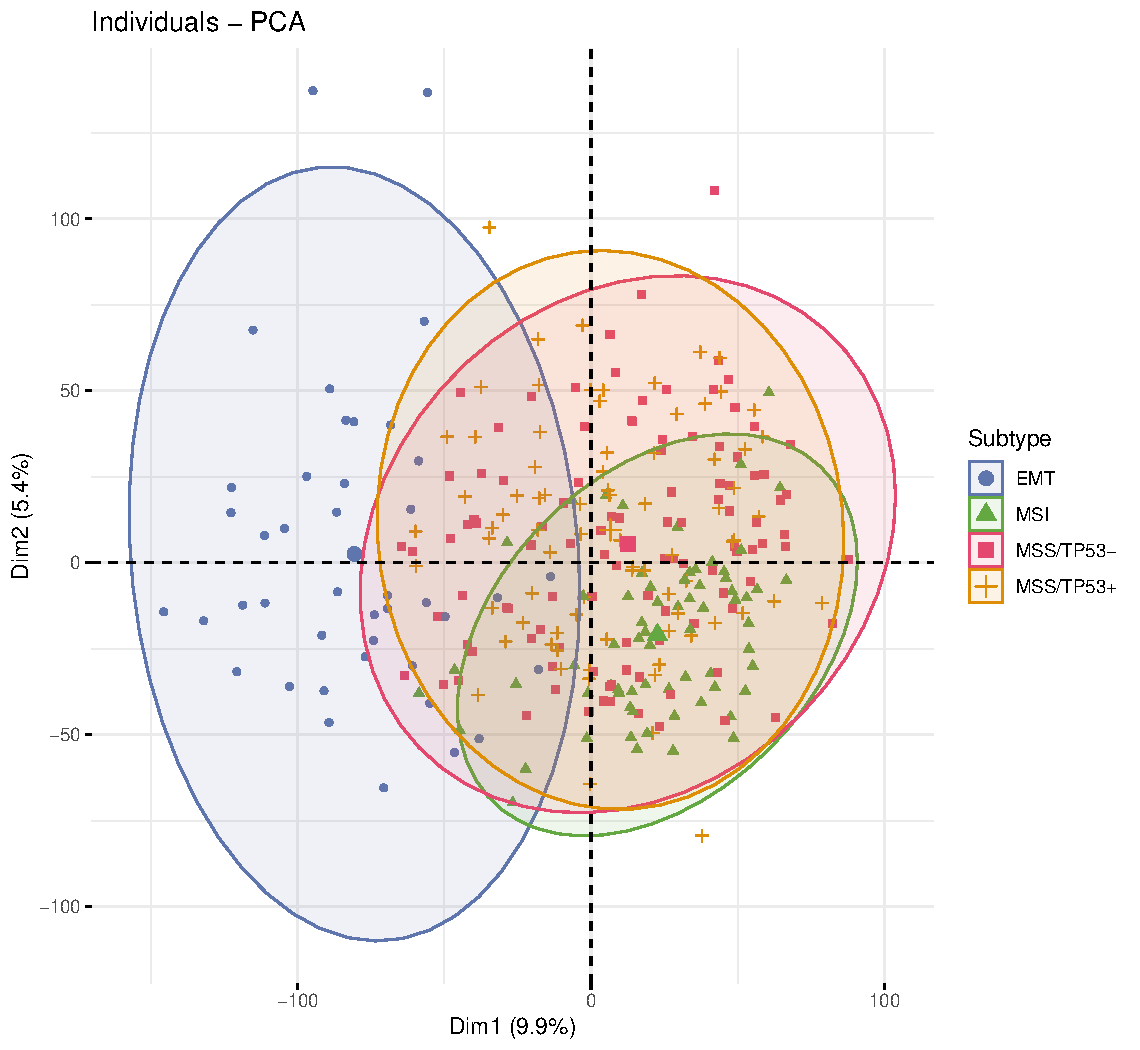
\includegraphics{tme-deg-gsea_files/figure-latex/unnamed-chunk-11-1.pdf}

\hypertarget{identifying-signatures-associated-with-tme-clusters}{%
\section{Identifying signatures associated with TME clusters}\label{identifying-signatures-associated-with-tme-clusters}}

Calculate TME associated signatures-(through PCA method).

\begin{Shaded}
\begin{Highlighting}[]
\NormalTok{sig\_tme}\OtherTok{\textless{}{-}}\FunctionTok{calculate\_sig\_score}\NormalTok{(}\AttributeTok{pdata           =} \ConstantTok{NULL}\NormalTok{,}
                             \AttributeTok{eset            =}\NormalTok{ eset,}
                             \AttributeTok{signature       =}\NormalTok{ signature\_collection,}
                             \AttributeTok{method          =} \StringTok{"pca"}\NormalTok{,}
                             \AttributeTok{mini\_gene\_count =} \DecValTok{2}\NormalTok{)}
\NormalTok{sig\_tme }\OtherTok{\textless{}{-}} \FunctionTok{t}\NormalTok{(}\FunctionTok{column\_to\_rownames}\NormalTok{(sig\_tme, }\AttributeTok{var =} \StringTok{"ID"}\NormalTok{))}
\NormalTok{sig\_tme[}\DecValTok{1}\SpecialCharTok{:}\DecValTok{5}\NormalTok{, }\DecValTok{1}\SpecialCharTok{:}\DecValTok{3}\NormalTok{]}
\end{Highlighting}
\end{Shaded}

\begin{verbatim}
##                   GSM1523727 GSM1523728 GSM1523729
## CD_8_T_effector   -2.5513794  0.7789141 -2.1770675
## DDR               -0.8747614  0.7425162 -1.3272054
## APM                1.1098368  2.1988688 -0.9516419
## Immune_Checkpoint -2.3701787  0.9455120 -1.4844104
## CellCycle_Reg      0.1063358  0.7583302 -0.3649795
\end{verbatim}

寻找与TMEcluster相关的特征变量

\begin{Shaded}
\begin{Highlighting}[]
\NormalTok{res }\OtherTok{\textless{}{-}} \FunctionTok{find\_markers\_in\_bulk}\NormalTok{(}\AttributeTok{pdata =}\NormalTok{ tme, }\AttributeTok{eset =}\NormalTok{ sig\_tme, }\AttributeTok{group =} \StringTok{"TMEcluster"}\NormalTok{, }\AttributeTok{nfeatures =} \DecValTok{1000}\NormalTok{, }\AttributeTok{top\_n =} \DecValTok{20}\NormalTok{, }\AttributeTok{min.pct =} \FloatTok{0.10}\NormalTok{)}
\end{Highlighting}
\end{Shaded}

\begin{verbatim}
## 
##  IA  IE  IS 
## 107  96  97 
## # A tibble: 58 x 7
## # Groups:   cluster [3]
##       p_val avg_log2FC pct.1 pct.2 p_val_adj cluster gene                       
##       <dbl>      <dbl> <dbl> <dbl>     <dbl> <fct>   <chr>                      
##  1 6.21e-19       4.07 0.701 0.316  1.59e-16 IA      IFNG-signature-Ayers-et-al 
##  2 1.82e-17       5.18 0.813 0.399  4.66e-15 IA      Th2-cells-Bindea-et-al     
##  3 2.60e-16       4.65 0.813 0.383  6.65e-14 IA      Folate-One-Carbon-Metaboli~
##  4 1.52e-15       5.12 0.804 0.352  3.89e-13 IA      Homologous-recombination   
##  5 4.95e-15       4.84 0.673 0.275  1.27e-12 IA      CD-8-T-effector            
##  6 7.70e-15       3.16 0.71  0.332  1.97e-12 IA      Th1-cells-Bindea-et-al     
##  7 9.52e-14       3.16 0.822 0.399  2.44e-11 IA      Purine-Biosynthesis        
##  8 1.42e-13       2.83 0.664 0.352  3.63e-11 IA      ADP-Ribosylation           
##  9 5.96e-13       2.96 0.785 0.42   1.53e-10 IA      TIP-Release-of-cancer-cell~
## 10 3.00e-12       2.71 0.776 0.409  7.68e-10 IA      Glycine--Serine-and-Threon~
## # i 48 more rows
\end{verbatim}

\begin{Shaded}
\begin{Highlighting}[]
\NormalTok{top15 }\OtherTok{\textless{}{-}}\NormalTok{  res}\SpecialCharTok{$}\NormalTok{top\_markers }\SpecialCharTok{\%\textgreater{}\%}\NormalTok{ dplyr}\SpecialCharTok{::} \FunctionTok{group\_by}\NormalTok{(cluster) }\SpecialCharTok{\%\textgreater{}\%}\NormalTok{  dplyr}\SpecialCharTok{::}\FunctionTok{top\_n}\NormalTok{(}\DecValTok{15}\NormalTok{, avg\_log2FC)}

\NormalTok{p1 }\OtherTok{\textless{}{-}} \FunctionTok{DoHeatmap}\NormalTok{(res}\SpecialCharTok{$}\NormalTok{sce, top15}\SpecialCharTok{$}\NormalTok{gene, }\AttributeTok{group.colors =}\NormalTok{ cols)}\SpecialCharTok{+}
  \FunctionTok{scale\_fill\_gradientn}\NormalTok{(}\AttributeTok{colours =} \FunctionTok{rev}\NormalTok{(}\FunctionTok{colorRampPalette}\NormalTok{(RColorBrewer}\SpecialCharTok{::}\FunctionTok{brewer.pal}\NormalTok{(}\DecValTok{11}\NormalTok{,}\StringTok{"RdBu"}\NormalTok{))(}\DecValTok{256}\NormalTok{)))}
\end{Highlighting}
\end{Shaded}

可视化结果:选择特征变量

\begin{Shaded}
\begin{Highlighting}[]
\NormalTok{top15}\SpecialCharTok{$}\NormalTok{gene  }\OtherTok{\textless{}{-}} \FunctionTok{gsub}\NormalTok{(top15}\SpecialCharTok{$}\NormalTok{gene, }\AttributeTok{pattern =} \StringTok{"}\SpecialCharTok{\textbackslash{}\textbackslash{}}\StringTok{{-}"}\NormalTok{, }\AttributeTok{replacement =} \StringTok{"}\SpecialCharTok{\textbackslash{}\textbackslash{}}\StringTok{\_"}\NormalTok{)}
\NormalTok{input }\OtherTok{\textless{}{-}} \FunctionTok{combine\_pd\_eset}\NormalTok{(}\AttributeTok{eset =}\NormalTok{ sig\_tme, }\AttributeTok{pdata =}\NormalTok{ tme, }\AttributeTok{feas =}\NormalTok{ top15}\SpecialCharTok{$}\NormalTok{gene, }\AttributeTok{scale =}\NormalTok{ T)}

\NormalTok{p2 }\OtherTok{\textless{}{-}} \FunctionTok{sig\_box}\NormalTok{(input, }\AttributeTok{variable =} \StringTok{"TMEcluster"}\NormalTok{, }\AttributeTok{signature =} \StringTok{"IFNG\_signature\_Ayers\_et\_al"}\NormalTok{, }\AttributeTok{jitter =} \ConstantTok{TRUE}\NormalTok{,}
              \AttributeTok{cols =}\NormalTok{  cols, }\AttributeTok{show\_pvalue =} \ConstantTok{TRUE}\NormalTok{, }\AttributeTok{size\_of\_pvalue =} \DecValTok{4}\NormalTok{, }\AttributeTok{size\_of\_font =} \DecValTok{6}\NormalTok{)}
\end{Highlighting}
\end{Shaded}

\begin{verbatim}
## # A tibble: 3 x 8
##   .y.       group1 group2        p   p.adj p.format p.signif method  
##   <chr>     <chr>  <chr>     <dbl>   <dbl> <chr>    <chr>    <chr>   
## 1 signature IA     IE     2.98e-13 6  e-13 3.0e-13  ****     Wilcoxon
## 2 signature IA     IS     1.85e-15 5.6e-15 1.9e-15  ****     Wilcoxon
## 3 signature IE     IS     2.68e- 1 2.7e- 1 0.27     ns       Wilcoxon
\end{verbatim}

\begin{Shaded}
\begin{Highlighting}[]
\NormalTok{p3 }\OtherTok{\textless{}{-}} \FunctionTok{sig\_box}\NormalTok{(input, }\AttributeTok{variable =} \StringTok{"TMEcluster"}\NormalTok{, }\AttributeTok{signature =} \StringTok{"Neutrophils\_Bindea\_et\_al"}\NormalTok{,  }
              \AttributeTok{jitter =} \ConstantTok{TRUE}\NormalTok{, }\AttributeTok{cols =}\NormalTok{  cols, }\AttributeTok{show\_pvalue =} \ConstantTok{TRUE}\NormalTok{, }\AttributeTok{size\_of\_pvalue =} \DecValTok{4}\NormalTok{, }\AttributeTok{size\_of\_font =} \DecValTok{6}\NormalTok{)}
\end{Highlighting}
\end{Shaded}

\begin{verbatim}
## # A tibble: 3 x 8
##   .y.       group1 group2         p   p.adj p.format p.signif method  
##   <chr>     <chr>  <chr>      <dbl>   <dbl> <chr>    <chr>    <chr>   
## 1 signature IA     IE     0.00639   0.013   0.0064   **       Wilcoxon
## 2 signature IA     IS     0.0584    0.058   0.0584   ns       Wilcoxon
## 3 signature IE     IS     0.0000929 0.00028 9.3e-05  ****     Wilcoxon
\end{verbatim}

\begin{Shaded}
\begin{Highlighting}[]
\NormalTok{p }\OtherTok{\textless{}{-}}\NormalTok{ (p1}\SpecialCharTok{|}\NormalTok{p2}\SpecialCharTok{/}\NormalTok{p3) }\SpecialCharTok{+} \FunctionTok{plot\_layout}\NormalTok{(}\AttributeTok{widths =} \FunctionTok{c}\NormalTok{(}\FloatTok{2.3}\NormalTok{,}\DecValTok{1}\NormalTok{))}
\NormalTok{p }\SpecialCharTok{+} \FunctionTok{plot\_annotation}\NormalTok{(}\AttributeTok{tag\_levels =} \StringTok{\textquotesingle{}A\textquotesingle{}}\NormalTok{)}
\end{Highlighting}
\end{Shaded}

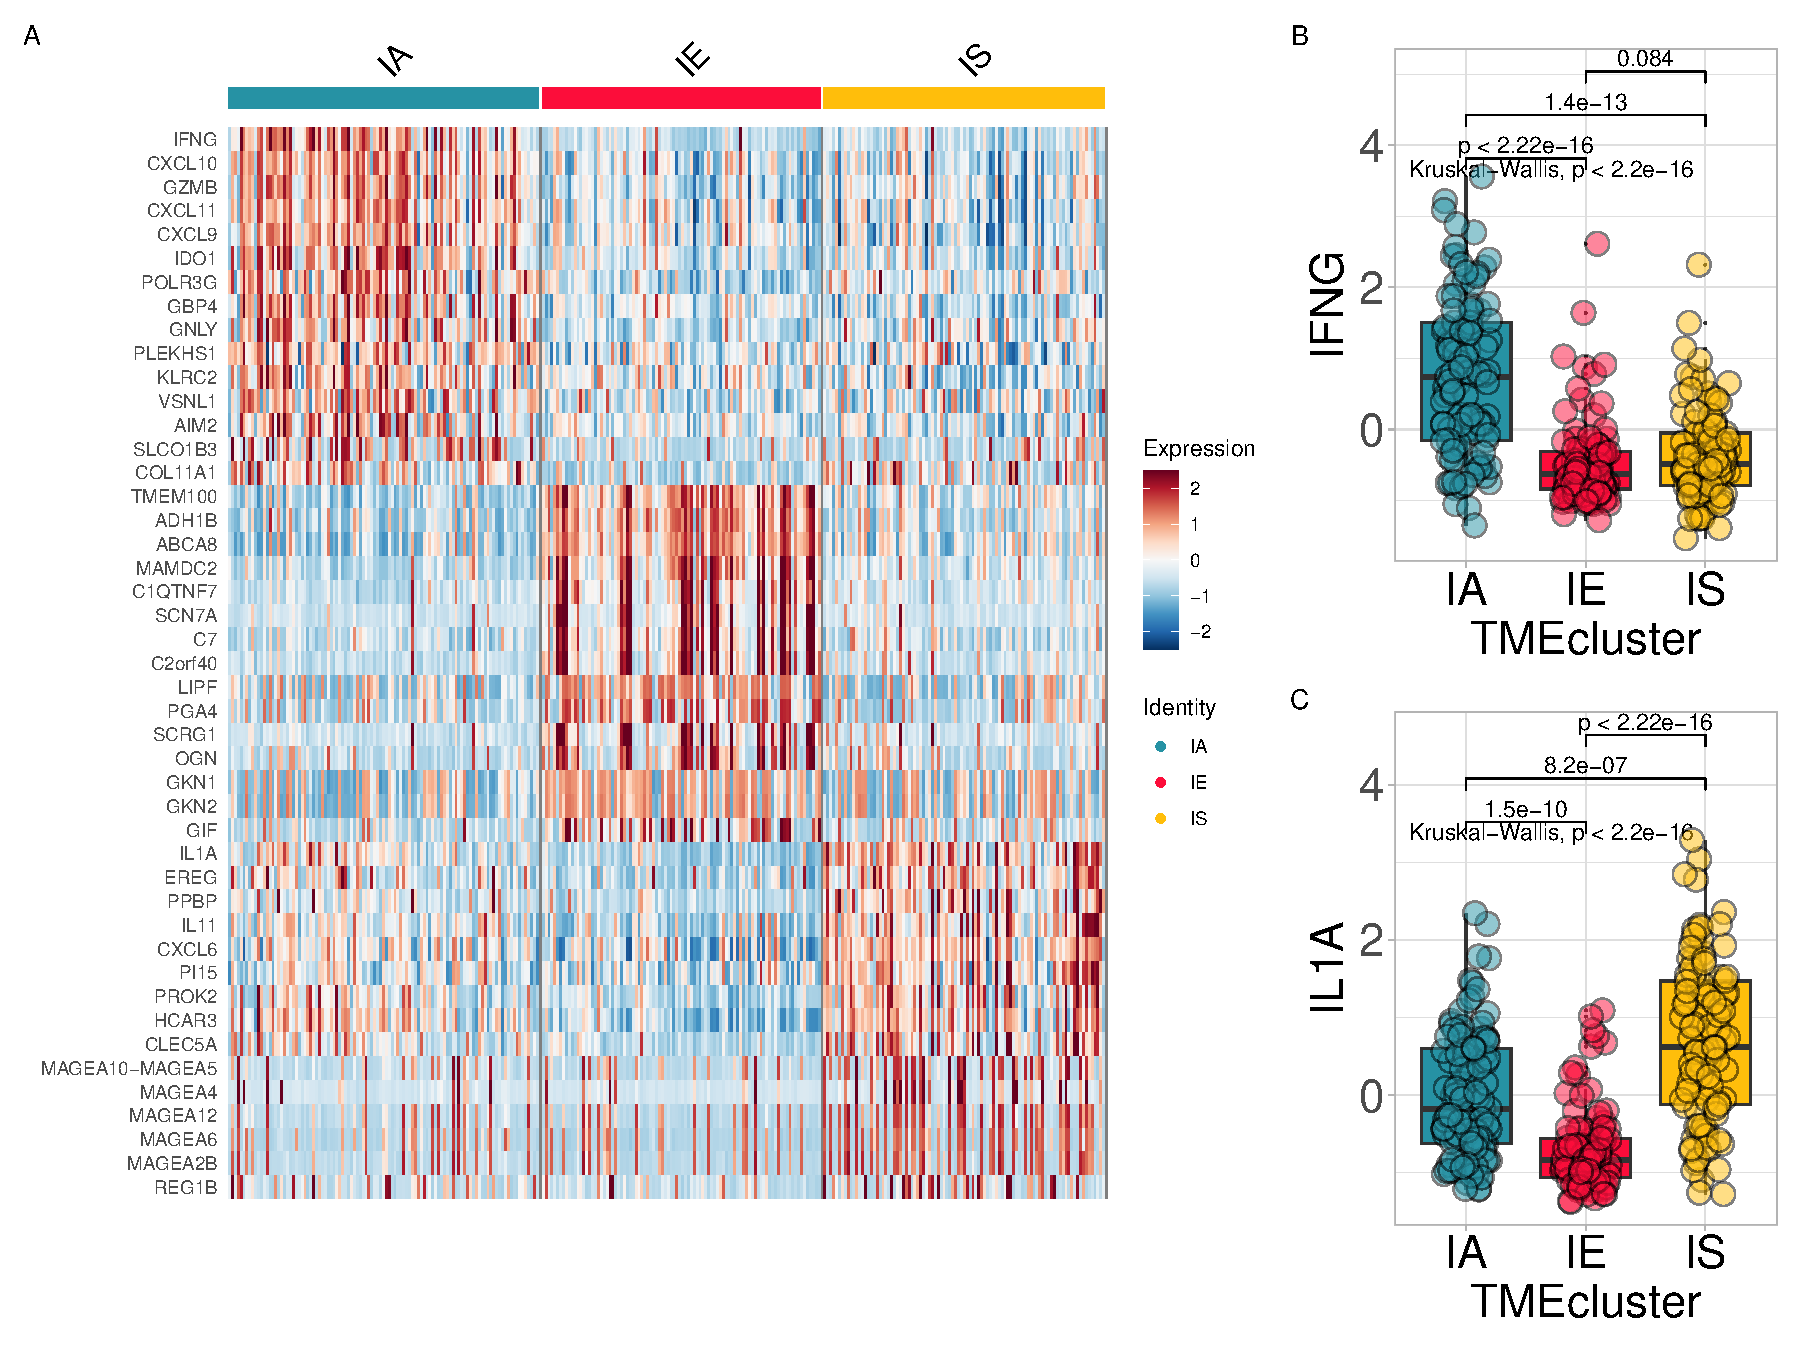
\includegraphics{tme-deg-gsea_files/figure-latex/unnamed-chunk-15-1.pdf}

\begin{Shaded}
\begin{Highlighting}[]
\FunctionTok{library}\NormalTok{(survminer)}
\end{Highlighting}
\end{Shaded}

\begin{verbatim}
## 
## Attaching package: 'survminer'
\end{verbatim}

\begin{verbatim}
## The following object is masked from 'package:survival':
## 
##     myeloma
\end{verbatim}

\begin{Shaded}
\begin{Highlighting}[]
\FunctionTok{data}\NormalTok{(pdata\_acrg, }\AttributeTok{package =} \StringTok{"IOBR"}\NormalTok{)}
\NormalTok{input }\OtherTok{\textless{}{-}} \FunctionTok{merge}\NormalTok{(pdata\_acrg, input, }\AttributeTok{by =} \StringTok{"ID"}\NormalTok{)}
\NormalTok{p1}\OtherTok{\textless{}{-}}\FunctionTok{surv\_group}\NormalTok{(}\AttributeTok{input\_pdata       =}\NormalTok{ input,}
               \AttributeTok{target\_group      =} \StringTok{"TMEcluster"}\NormalTok{,}
               \AttributeTok{ID                =} \StringTok{"ID"}\NormalTok{,}
               \AttributeTok{reference\_group   =} \StringTok{"High"}\NormalTok{,}
               \AttributeTok{project           =} \StringTok{"ACRG"}\NormalTok{,}
               \AttributeTok{cols              =}\NormalTok{ cols, }
               \AttributeTok{time              =} \StringTok{"OS\_time"}\NormalTok{,}
               \AttributeTok{status            =} \StringTok{"OS\_status"}\NormalTok{,}
               \AttributeTok{time\_type         =} \StringTok{"month"}\NormalTok{,}
               \AttributeTok{save\_path         =} \StringTok{"result"}\NormalTok{)}
\end{Highlighting}
\end{Shaded}

\begin{verbatim}
## >>> Dataset's survival follow up time is range between 1 to 105.7 months
\end{verbatim}

\begin{verbatim}
##  IA  IE  IS 
## 107  96  97
\end{verbatim}

\begin{verbatim}
## 1079697
\end{verbatim}

\begin{verbatim}
##   Maximum of follow up time is 105.7 months; and will be divided into 6 sections;
\end{verbatim}

\begin{Shaded}
\begin{Highlighting}[]
\NormalTok{p1}
\end{Highlighting}
\end{Shaded}

\includegraphics{tme-deg-gsea_files/figure-latex/unnamed-chunk-16-1.pdf}

\begin{Shaded}
\begin{Highlighting}[]
\NormalTok{p1}\OtherTok{\textless{}{-}} \FunctionTok{percent\_bar\_plot}\NormalTok{(input, }\AttributeTok{x =} \StringTok{"TMEcluster"}\NormalTok{ , }\AttributeTok{y =} \StringTok{"Subtype"}\NormalTok{, }\AttributeTok{palette =} \StringTok{"jama"}\NormalTok{)}
\end{Highlighting}
\end{Shaded}

\begin{verbatim}
## # A tibble: 12 x 5
## # Groups:   TMEcluster [3]
##    TMEcluster Subtype    Freq  Prop count
##    <chr>      <fct>     <dbl> <dbl> <dbl>
##  1 IA         EMT           7  0.07   107
##  2 IA         MSI          49  0.46   107
##  3 IA         MSS/TP53-    27  0.25   107
##  4 IA         MSS/TP53+    24  0.22   107
##  5 IE         EMT          24  0.25    96
##  6 IE         MSI           3  0.03    96
##  7 IE         MSS/TP53-    40  0.42    96
##  8 IE         MSS/TP53+    29  0.3     96
##  9 IS         EMT          15  0.15    97
## 10 IS         MSI          16  0.16    97
## 11 IS         MSS/TP53-    40  0.41    97
## 12 IS         MSS/TP53+    26  0.27    97
## [1] "'#374E55FF', '#DF8F44FF', '#00A1D5FF', '#B24745FF', '#79AF97FF', '#6A6599FF', '#80796BFF'"
\end{verbatim}

\begin{Shaded}
\begin{Highlighting}[]
\NormalTok{p2}\OtherTok{\textless{}{-}} \FunctionTok{percent\_bar\_plot}\NormalTok{(input, }\AttributeTok{x =} \StringTok{"TMEcluster"}\NormalTok{ , }\AttributeTok{y =} \StringTok{"Lauren"}\NormalTok{, }\AttributeTok{palette =} \StringTok{"jama"}\NormalTok{)}
\end{Highlighting}
\end{Shaded}

\begin{verbatim}
## # A tibble: 9 x 5
## # Groups:   TMEcluster [3]
##   TMEcluster Lauren      Freq  Prop count
##   <chr>      <fct>      <dbl> <dbl> <dbl>
## 1 IA         Diffuse       34  0.32   107
## 2 IA         Intestinal    60  0.56   107
## 3 IA         Mixed         13  0.12   107
## 4 IE         Diffuse       60  0.62    96
## 5 IE         Intestinal    32  0.33    96
## 6 IE         Mixed          4  0.04    96
## 7 IS         Diffuse       41  0.42    97
## 8 IS         Intestinal    54  0.56    97
## 9 IS         Mixed          2  0.02    97
## [1] "'#374E55FF', '#DF8F44FF', '#00A1D5FF', '#B24745FF', '#79AF97FF', '#6A6599FF', '#80796BFF'"
\end{verbatim}

\begin{Shaded}
\begin{Highlighting}[]
\NormalTok{p3}\OtherTok{\textless{}{-}} \FunctionTok{percent\_bar\_plot}\NormalTok{(input, }\AttributeTok{x =} \StringTok{"TMEcluster"}\NormalTok{ , }\AttributeTok{y =} \StringTok{"TMEscore\_binary"}\NormalTok{, }\AttributeTok{palette =} \StringTok{"jama"}\NormalTok{)}
\end{Highlighting}
\end{Shaded}

\begin{verbatim}
## # A tibble: 7 x 5
## # Groups:   TMEcluster [3]
##   TMEcluster TMEscore_binary  Freq  Prop count
##   <chr>      <fct>           <dbl> <dbl> <dbl>
## 1 IA         High               60  0.56   107
## 2 IA         Low                47  0.44   107
## 3 IE         High                5  0.05    96
## 4 IE         Low                91  0.95    96
## 5 IS         High                6  0.06    97
## 6 IS         Low                90  0.93    97
## 7 IS         <NA>                1  0.01    97
## [1] "'#374E55FF', '#DF8F44FF', '#00A1D5FF', '#B24745FF', '#79AF97FF', '#6A6599FF', '#80796BFF'"
\end{verbatim}

\begin{Shaded}
\begin{Highlighting}[]
\NormalTok{p1}\SpecialCharTok{|}\NormalTok{p2}\SpecialCharTok{|}\NormalTok{p3}
\end{Highlighting}
\end{Shaded}

\includegraphics{tme-deg-gsea_files/figure-latex/unnamed-chunk-18-1.pdf}

\hypertarget{signature-and-relevant-phenotypes}{%
\chapter{\texorpdfstring{\textbf{Signature and relevant phenotypes}}{Signature and relevant phenotypes}}\label{signature-and-relevant-phenotypes}}

\hypertarget{loading-packages-2}{%
\section{Loading packages}\label{loading-packages-2}}

Load the IOBR package in your R session after the installation is complete:

\begin{Shaded}
\begin{Highlighting}[]
\FunctionTok{library}\NormalTok{(IOBR)}
\FunctionTok{library}\NormalTok{(survminer)}
\FunctionTok{library}\NormalTok{(tidyverse)}
\end{Highlighting}
\end{Shaded}

\hypertarget{downloading-data-for-example-2}{%
\section{Downloading data for example}\label{downloading-data-for-example-2}}

Obtaining data set from GEO \href{https://pubmed.ncbi.nlm.nih.gov/25894828/}{Gastric cancer: GSE62254} using \texttt{GEOquery} R package.

\begin{Shaded}
\begin{Highlighting}[]
\ControlFlowTok{if}\NormalTok{ (}\SpecialCharTok{!}\FunctionTok{requireNamespace}\NormalTok{(}\StringTok{"GEOquery"}\NormalTok{, }\AttributeTok{quietly =} \ConstantTok{TRUE}\NormalTok{))  BiocManager}\SpecialCharTok{::}\FunctionTok{install}\NormalTok{(}\StringTok{"GEOquery"}\NormalTok{)}
\FunctionTok{library}\NormalTok{(}\StringTok{"GEOquery"}\NormalTok{)}
\CommentTok{\# }\AlertTok{NOTE}\CommentTok{: This process may take a few minutes which depends on the internet connection speed. Please wait for its completion.}
\NormalTok{eset\_geo }\OtherTok{\textless{}{-}} \FunctionTok{getGEO}\NormalTok{(}\AttributeTok{GEO =} \StringTok{"GSE62254"}\NormalTok{, }\AttributeTok{getGPL  =}\NormalTok{ F, }\AttributeTok{destdir =} \StringTok{"./"}\NormalTok{)}
\NormalTok{eset    }\OtherTok{\textless{}{-}}\NormalTok{eset\_geo[[}\DecValTok{1}\NormalTok{]]}
\NormalTok{eset    }\OtherTok{\textless{}{-}}\FunctionTok{exprs}\NormalTok{(eset)}
\NormalTok{eset[}\DecValTok{1}\SpecialCharTok{:}\DecValTok{5}\NormalTok{,}\DecValTok{1}\SpecialCharTok{:}\DecValTok{5}\NormalTok{]}
\end{Highlighting}
\end{Shaded}

\begin{verbatim}
##           GSM1523727 GSM1523728 GSM1523729 GSM1523744 GSM1523745
## 1007_s_at  3.2176645  3.0624323  3.0279131   2.921683  2.8456013
## 1053_at    2.4050109  2.4394879  2.2442708   2.345916  2.4328582
## 117_at     1.4933412  1.8067380  1.5959665   1.839822  1.8326058
## 121_at     2.1965561  2.2812181  2.1865556   2.258599  2.1874363
## 1255_g_at  0.8698382  0.9502466  0.8125414   1.012860  0.9441993
\end{verbatim}

Annotation of genes in the expression matrix and removal of duplicate genes.

\begin{Shaded}
\begin{Highlighting}[]
\CommentTok{\# Load the annotation file \textasciigrave{}anno\_hug133plus2\textasciigrave{} in IOBR.}
\FunctionTok{head}\NormalTok{(anno\_hug133plus2)}
\end{Highlighting}
\end{Shaded}

\begin{verbatim}
## # A tibble: 6 x 2
##   probe_id  symbol 
##   <fct>     <fct>  
## 1 1007_s_at MIR4640
## 2 1053_at   RFC2   
## 3 117_at    HSPA6  
## 4 121_at    PAX8   
## 5 1255_g_at GUCA1A 
## 6 1294_at   MIR5193
\end{verbatim}

\begin{Shaded}
\begin{Highlighting}[]
\CommentTok{\# Conduct gene annotation using \textasciigrave{}anno\_hug133plus2\textasciigrave{} file; If identical gene symbols exists, these genes would be ordered by the mean expression levels. The gene symbol with highest mean expression level is selected and remove others. }

\NormalTok{eset}\OtherTok{\textless{}{-}}\FunctionTok{anno\_eset}\NormalTok{(}\AttributeTok{eset       =}\NormalTok{ eset,}
                \AttributeTok{annotation =}\NormalTok{ anno\_hug133plus2,}
                \AttributeTok{symbol     =} \StringTok{"symbol"}\NormalTok{,}
                \AttributeTok{probe      =} \StringTok{"probe\_id"}\NormalTok{,}
                \AttributeTok{method     =} \StringTok{"mean"}\NormalTok{)}
\NormalTok{eset[}\DecValTok{1}\SpecialCharTok{:}\DecValTok{5}\NormalTok{, }\DecValTok{1}\SpecialCharTok{:}\DecValTok{3}\NormalTok{]}
\end{Highlighting}
\end{Shaded}

\begin{verbatim}
##              GSM1523727 GSM1523728 GSM1523729
## SH3KBP1        4.327974   4.316195   4.351425
## RPL41          4.246149   4.246808   4.257940
## EEF1A1         4.293762   4.291038   4.262199
## COX2           4.250288   4.283714   4.270508
## LOC101928826   4.219303   4.219670   4.213252
\end{verbatim}

\hypertarget{signature-score-estimation}{%
\section{Signature score estimation}\label{signature-score-estimation}}

\hypertarget{signature-collection-of-iobr}{%
\subsection{Signature collection of IOBR}\label{signature-collection-of-iobr}}

\begin{Shaded}
\begin{Highlighting}[]
\CommentTok{\# Return available parameter options of signature estimation.}
\NormalTok{signature\_score\_calculation\_methods}
\end{Highlighting}
\end{Shaded}

\begin{verbatim}
##           PCA        ssGSEA       z-score   Integration 
##         "pca"      "ssgsea"      "zscore" "integration"
\end{verbatim}

\begin{Shaded}
\begin{Highlighting}[]
\CommentTok{\#TME associated signatures}
\FunctionTok{names}\NormalTok{(signature\_tme)[}\DecValTok{1}\SpecialCharTok{:}\DecValTok{20}\NormalTok{]}
\end{Highlighting}
\end{Shaded}

\begin{verbatim}
##  [1] "CD_8_T_effector"            "DDR"                       
##  [3] "APM"                        "Immune_Checkpoint"         
##  [5] "CellCycle_Reg"              "Pan_F_TBRs"                
##  [7] "Histones"                   "EMT1"                      
##  [9] "EMT2"                       "EMT3"                      
## [11] "WNT_target"                 "FGFR3_related"             
## [13] "Cell_cycle"                 "Mismatch_Repair"           
## [15] "Homologous_recombination"   "Nucleotide_excision_repair"
## [17] "DNA_replication"            "Base_excision_repair"      
## [19] "TMEscoreA_CIR"              "TMEscoreB_CIR"
\end{verbatim}

\begin{Shaded}
\begin{Highlighting}[]
\CommentTok{\#Metabolism related signatures}
\FunctionTok{names}\NormalTok{(signature\_metabolism)[}\DecValTok{1}\SpecialCharTok{:}\DecValTok{20}\NormalTok{]}
\end{Highlighting}
\end{Shaded}

\begin{verbatim}
##  [1] "Cardiolipin_Metabolism"                    
##  [2] "Cardiolipin_Biosynthesis"                  
##  [3] "Cholesterol_Biosynthesis"                  
##  [4] "Citric_Acid_Cycle"                         
##  [5] "Cyclooxygenase_Arachidonic_Acid_Metabolism"
##  [6] "Prostaglandin_Biosynthesis"                
##  [7] "Purine_Biosynthesis"                       
##  [8] "Pyrimidine_Biosynthesis"                   
##  [9] "Dopamine_Biosynthesis"                     
## [10] "Epinephrine_Biosynthesis"                  
## [11] "Norepinephrine_Biosynthesis"               
## [12] "Fatty_Acid_Degradation"                    
## [13] "Fatty_Acid_Elongation"                     
## [14] "Fatty_Acid_Biosynthesis"                   
## [15] "Folate_One_Carbon_Metabolism"              
## [16] "Folate_biosynthesis"                       
## [17] "Gluconeogenesis"                           
## [18] "Glycolysis"                                
## [19] "Glycogen_Biosynthesis"                     
## [20] "Glycogen_Degradation"
\end{verbatim}

\begin{Shaded}
\begin{Highlighting}[]
\CommentTok{\#Signatures associated with biomedical basic research: such as m6A and exosomes}
\FunctionTok{names}\NormalTok{(signature\_tumor)}
\end{Highlighting}
\end{Shaded}

\begin{verbatim}
##  [1] "Nature_metabolism_Hypoxia"                
##  [2] "Winter_hypoxia_signature"                 
##  [3] "Hu_hypoxia_signature"                     
##  [4] "Molecular_Cancer_m6A"                     
##  [5] "MT_exosome"                               
##  [6] "SR_exosome"                               
##  [7] "Positive_regulation_of_exosomal_secretion"
##  [8] "Negative_regulation_of_exosomal_secretion"
##  [9] "Exosomal_secretion"                       
## [10] "Exosome_assembly"                         
## [11] "Extracellular_vesicle_biogenesis"         
## [12] "MC_Review_Exosome1"                       
## [13] "MC_Review_Exosome2"                       
## [14] "CMLS_Review_Exosome"                      
## [15] "Ferroptosis"                              
## [16] "EV_Cell_2020"
\end{verbatim}

\begin{Shaded}
\begin{Highlighting}[]
\CommentTok{\#signature collection including all aforementioned signatures }
\FunctionTok{names}\NormalTok{(signature\_collection)[}\DecValTok{1}\SpecialCharTok{:}\DecValTok{20}\NormalTok{]}
\end{Highlighting}
\end{Shaded}

\begin{verbatim}
##  [1] "CD_8_T_effector"            "DDR"                       
##  [3] "APM"                        "Immune_Checkpoint"         
##  [5] "CellCycle_Reg"              "Pan_F_TBRs"                
##  [7] "Histones"                   "EMT1"                      
##  [9] "EMT2"                       "EMT3"                      
## [11] "WNT_target"                 "FGFR3_related"             
## [13] "Cell_cycle"                 "Mismatch_Repair"           
## [15] "Homologous_recombination"   "Nucleotide_excision_repair"
## [17] "DNA_replication"            "Base_excision_repair"      
## [19] "TMEscoreA_CIR"              "TMEscoreB_CIR"
\end{verbatim}

\begin{Shaded}
\begin{Highlighting}[]
\CommentTok{\#citation of signatures}
\NormalTok{signature\_collection\_citation[}\DecValTok{1}\SpecialCharTok{:}\DecValTok{20}\NormalTok{, ]}
\end{Highlighting}
\end{Shaded}

\begin{verbatim}
## # A tibble: 20 x 6
##    Signatures                 `Published year` Journal         Title PMID  DOI  
##    <chr>                                 <dbl> <chr>           <chr> <chr> <chr>
##  1 CD_8_T_effector                        2018 Nature          TGFβ~ 2944~ 10.1~
##  2 DDR                                    2018 Nature          TGFβ~ 2944~ 10.1~
##  3 APM                                    2018 Nature          TGFβ~ 2944~ 10.1~
##  4 Immune_Checkpoint                      2018 Nature          TGFβ~ 2944~ 10.1~
##  5 CellCycle_Reg                          2018 Nature          TGFβ~ 2944~ 10.1~
##  6 Pan_F_TBRs                             2018 Nature          TGFβ~ 2944~ 10.1~
##  7 Histones                               2018 Nature          TGFβ~ 2944~ 10.1~
##  8 EMT1                                   2018 Nature          TGFβ~ 2944~ 10.1~
##  9 EMT2                                   2018 Nature          TGFβ~ 2944~ 10.1~
## 10 EMT3                                   2018 Nature          TGFβ~ 2944~ 10.1~
## 11 WNT_target                             2018 Nature          TGFβ~ 2944~ 10.1~
## 12 FGFR3_related                          2018 Nature          TGFβ~ 2944~ 10.1~
## 13 Cell_cycle                             2018 Nature          TGFβ~ 2944~ 10.1~
## 14 Mismatch_Repair                        2018 Nature          TGFβ~ 2944~ 10.1~
## 15 Homologous_recombination               2018 Nature          TGFβ~ 2944~ 10.1~
## 16 Nucleotide_excision_repair             2018 Nature          TGFβ~ 2944~ 10.1~
## 17 DNA_replication                        2018 Nature          TGFβ~ 2944~ 10.1~
## 18 Base_excision_repair                   2018 Nature          TGFβ~ 2944~ 10.1~
## 19 TMEscoreA_CIR                          2019 Cancer Immunol~ Tumo~ 3084~ 10.1~
## 20 TMEscoreB_CIR                          2019 Cancer Immunol~ Tumo~ 3084~ 10.1~
\end{verbatim}

Three methodologies were adopted in the process of signature score evaluation, comprising Single-sample Gene Set Enrichment Analysis (ssGSEA), Principal component analysis (PCA), and Z-score.

\hypertarget{estimated-by-pca-method}{%
\subsection{Estimated by PCA method}\label{estimated-by-pca-method}}

\begin{Shaded}
\begin{Highlighting}[]
\NormalTok{sig\_tme}\OtherTok{\textless{}{-}}\FunctionTok{calculate\_sig\_score}\NormalTok{(}\AttributeTok{pdata           =} \ConstantTok{NULL}\NormalTok{,}
                             \AttributeTok{eset            =}\NormalTok{ eset,}
                             \AttributeTok{signature       =}\NormalTok{ signature\_collection,}
                             \AttributeTok{method          =} \StringTok{"pca"}\NormalTok{,}
                             \AttributeTok{mini\_gene\_count =} \DecValTok{2}\NormalTok{)}

\NormalTok{sig\_tme }\OtherTok{\textless{}{-}} \FunctionTok{t}\NormalTok{(}\FunctionTok{column\_to\_rownames}\NormalTok{(sig\_tme, }\AttributeTok{var =} \StringTok{"ID"}\NormalTok{))}
\NormalTok{sig\_tme[}\DecValTok{1}\SpecialCharTok{:}\DecValTok{5}\NormalTok{, }\DecValTok{1}\SpecialCharTok{:}\DecValTok{3}\NormalTok{]}
\end{Highlighting}
\end{Shaded}

\begin{verbatim}
##                   GSM1523727 GSM1523728 GSM1523729
## CD_8_T_effector   -2.5513794  0.7789141 -2.1770675
## DDR               -0.8747614  0.7425162 -1.3272054
## APM                1.1098368  2.1988688 -0.9516419
## Immune_Checkpoint -2.3701787  0.9455120 -1.4844104
## CellCycle_Reg      0.1063358  0.7583302 -0.3649795
\end{verbatim}

\hypertarget{estimated-by-ssgsea-methodology}{%
\subsection{Estimated by ssGSEA methodology}\label{estimated-by-ssgsea-methodology}}

This method is suitable for gene sets with a large number of genes, such as those of \href{https://www.gsea-msigdb.org/gsea/msigdb}{GO, KEGG, REACTOME gene sets}.

\begin{figure}

{\centering 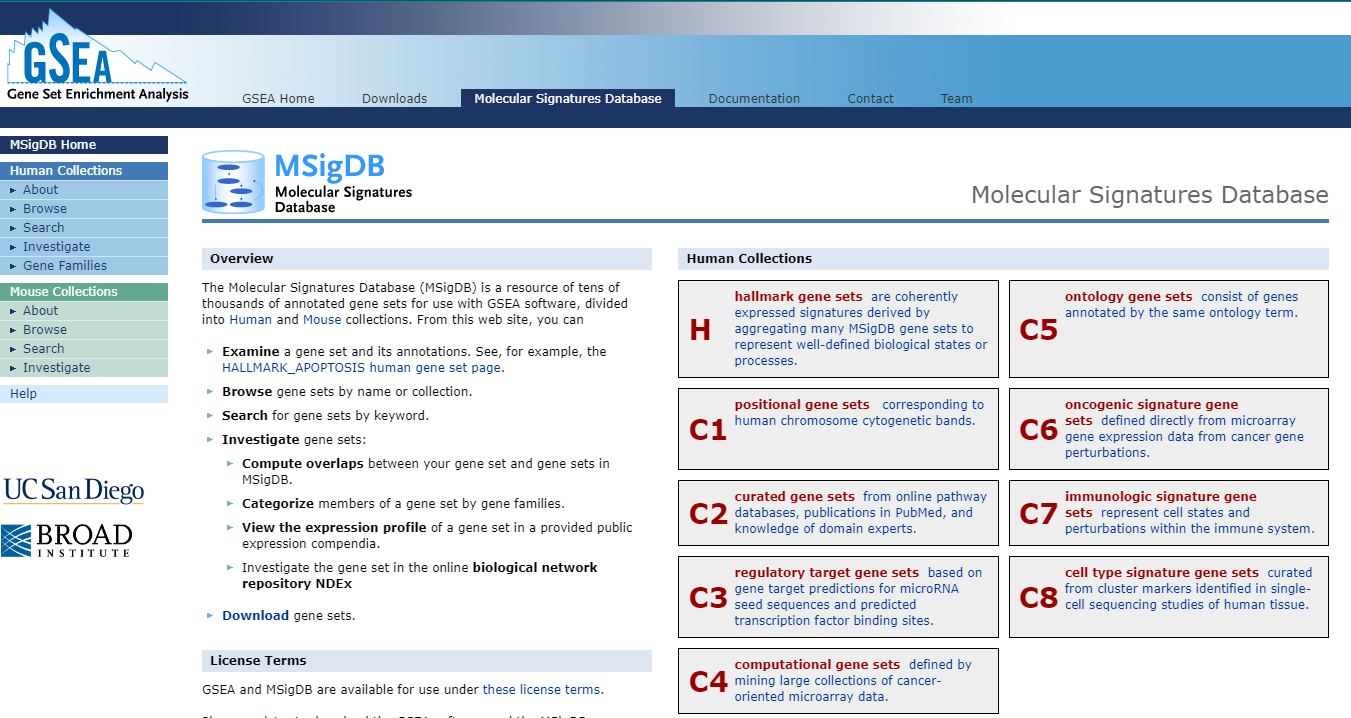
\includegraphics[width=0.95\linewidth]{./fig/gsea} 

}

\caption{The workflow of IOBR}\label{fig:unnamed-chunk-10}
\end{figure}

\begin{Shaded}
\begin{Highlighting}[]
\NormalTok{sig\_tme}\OtherTok{\textless{}{-}}\FunctionTok{calculate\_sig\_score}\NormalTok{(}\AttributeTok{pdata           =} \ConstantTok{NULL}\NormalTok{,}
                             \AttributeTok{eset            =}\NormalTok{ eset,}
                             \AttributeTok{signature       =}\NormalTok{ go\_bp,}
                             \AttributeTok{method          =} \StringTok{"ssgsea"}\NormalTok{,}
                             \AttributeTok{mini\_gene\_count =} \DecValTok{2}\NormalTok{)}
\end{Highlighting}
\end{Shaded}

\hypertarget{estimated-by-zscore-function}{%
\subsection{Estimated by zscore function}\label{estimated-by-zscore-function}}

\begin{Shaded}
\begin{Highlighting}[]
\NormalTok{sig\_tme}\OtherTok{\textless{}{-}}\FunctionTok{calculate\_sig\_score}\NormalTok{(}\AttributeTok{pdata           =} \ConstantTok{NULL}\NormalTok{,}
                             \AttributeTok{eset            =}\NormalTok{ eset,}
                             \AttributeTok{signature       =}\NormalTok{ signature\_collection,}
                             \AttributeTok{method          =} \StringTok{"zscore"}\NormalTok{,}
                             \AttributeTok{mini\_gene\_count =} \DecValTok{2}\NormalTok{)}
\end{Highlighting}
\end{Shaded}

\hypertarget{reference}{%
\subsection{Reference}\label{reference}}

\textbf{ssgsea}: Barbie, D.A. et al (2009). Systematic RNA interference reveals that oncogenic KRAS-driven cancers require TBK1. Nature, 462(5):108-112.

\textbf{gsva}: Hänzelmann, S., Castelo, R. and Guinney, J. (2013). GSVA: Gene set variation analysis for microarray and RNA-Seq data. BMC Bioinformatics, 14(1):7.

\textbf{zscore}: Lee, E. et al (2008). Inferring pathway activity toward precise disease classification. PLoS Comp Biol, 4(11):e1000217.

\textbf{PCA method}: Mariathasan S, Turley SJ, Nickles D, et al.~TGFβ attenuates tumour response to PD-L1 blockade by contributing to exclusion of T cells. Nature. 2018 Feb 22;554(7693):544-548.

\hypertarget{identifying-features-associated-with-survival}{%
\section{Identifying features associated with survival}\label{identifying-features-associated-with-survival}}

\begin{Shaded}
\begin{Highlighting}[]
\FunctionTok{data}\NormalTok{(}\StringTok{"pdata\_acrg"}\NormalTok{)}
\NormalTok{input }\OtherTok{\textless{}{-}} \FunctionTok{combine\_pd\_eset}\NormalTok{(}\AttributeTok{eset =}\NormalTok{ sig\_tme, }\AttributeTok{pdata =}\NormalTok{ pdata\_acrg, }\AttributeTok{scale =}\NormalTok{ T)}
\NormalTok{res}\OtherTok{\textless{}{-}} \FunctionTok{batch\_surv}\NormalTok{(}\AttributeTok{pdata    =}\NormalTok{ input,}
                 \AttributeTok{time     =} \StringTok{"OS\_time"}\NormalTok{, }
                 \AttributeTok{status   =} \StringTok{"OS\_status"}\NormalTok{, }
                 \AttributeTok{variable =} \FunctionTok{colnames}\NormalTok{(input)[}\DecValTok{69}\SpecialCharTok{:}\FunctionTok{ncol}\NormalTok{(input)])}
\FunctionTok{head}\NormalTok{(res)}
\end{Highlighting}
\end{Shaded}

\begin{verbatim}
## # A tibble: 6 x 5
##   ID                           P    HR CI_low_0.95 CI_up_0.95
##   <chr>                    <dbl> <dbl>       <dbl>      <dbl>
## 1 Folate_biosynthesis   1.00e-10 0.579       0.490      0.683
## 2 TMEscore_CIR          1.32e- 9 0.640       0.554      0.739
## 3 Glycogen_Biosynthesis 3.24e- 9 1.52        1.32       1.74 
## 4 Pan_F_TBRs            6.33e- 9 1.55        1.34       1.80 
## 5 TMEscoreB_CIR         7.17e- 9 1.52        1.32       1.75 
## 6 TMEscore_plus         8.08e- 9 0.638       0.547      0.743
\end{verbatim}

\begin{Shaded}
\begin{Highlighting}[]
\NormalTok{res}\OtherTok{\textless{}{-}}\NormalTok{ res[}\FunctionTok{nchar}\NormalTok{(res}\SpecialCharTok{$}\NormalTok{ID)}\SpecialCharTok{\textless{}=}\DecValTok{28}\NormalTok{, ]}
\NormalTok{p1}\OtherTok{\textless{}{-}} \FunctionTok{sig\_forest}\NormalTok{(res, }\AttributeTok{signature =} \StringTok{"ID"}\NormalTok{, }\AttributeTok{n =} \DecValTok{20}\NormalTok{)}
\end{Highlighting}
\end{Shaded}

\begin{center}\includegraphics{signature-analysis_files/figure-latex/unnamed-chunk-13-1} \end{center}

\hypertarget{visulization-using-heatmap}{%
\section{Visulization using heatmap}\label{visulization-using-heatmap}}

Signatures和分子分型之间的关系
使用\texttt{IOBR}的\texttt{sig\_heatmap}进行热图的可视化

\begin{Shaded}
\begin{Highlighting}[]
\NormalTok{p2 }\OtherTok{\textless{}{-}} \FunctionTok{sig\_heatmap}\NormalTok{(}\AttributeTok{input         =}\NormalTok{ input, }
                  \AttributeTok{features      =}\NormalTok{ res}\SpecialCharTok{$}\NormalTok{ID[}\DecValTok{1}\SpecialCharTok{:}\DecValTok{20}\NormalTok{],}
                  \AttributeTok{group         =} \StringTok{"Subtype"}\NormalTok{, }
                  \AttributeTok{palette\_group =} \StringTok{"jama"}\NormalTok{, }
                  \AttributeTok{palette       =} \DecValTok{6}\NormalTok{)}
\end{Highlighting}
\end{Shaded}

\begin{center}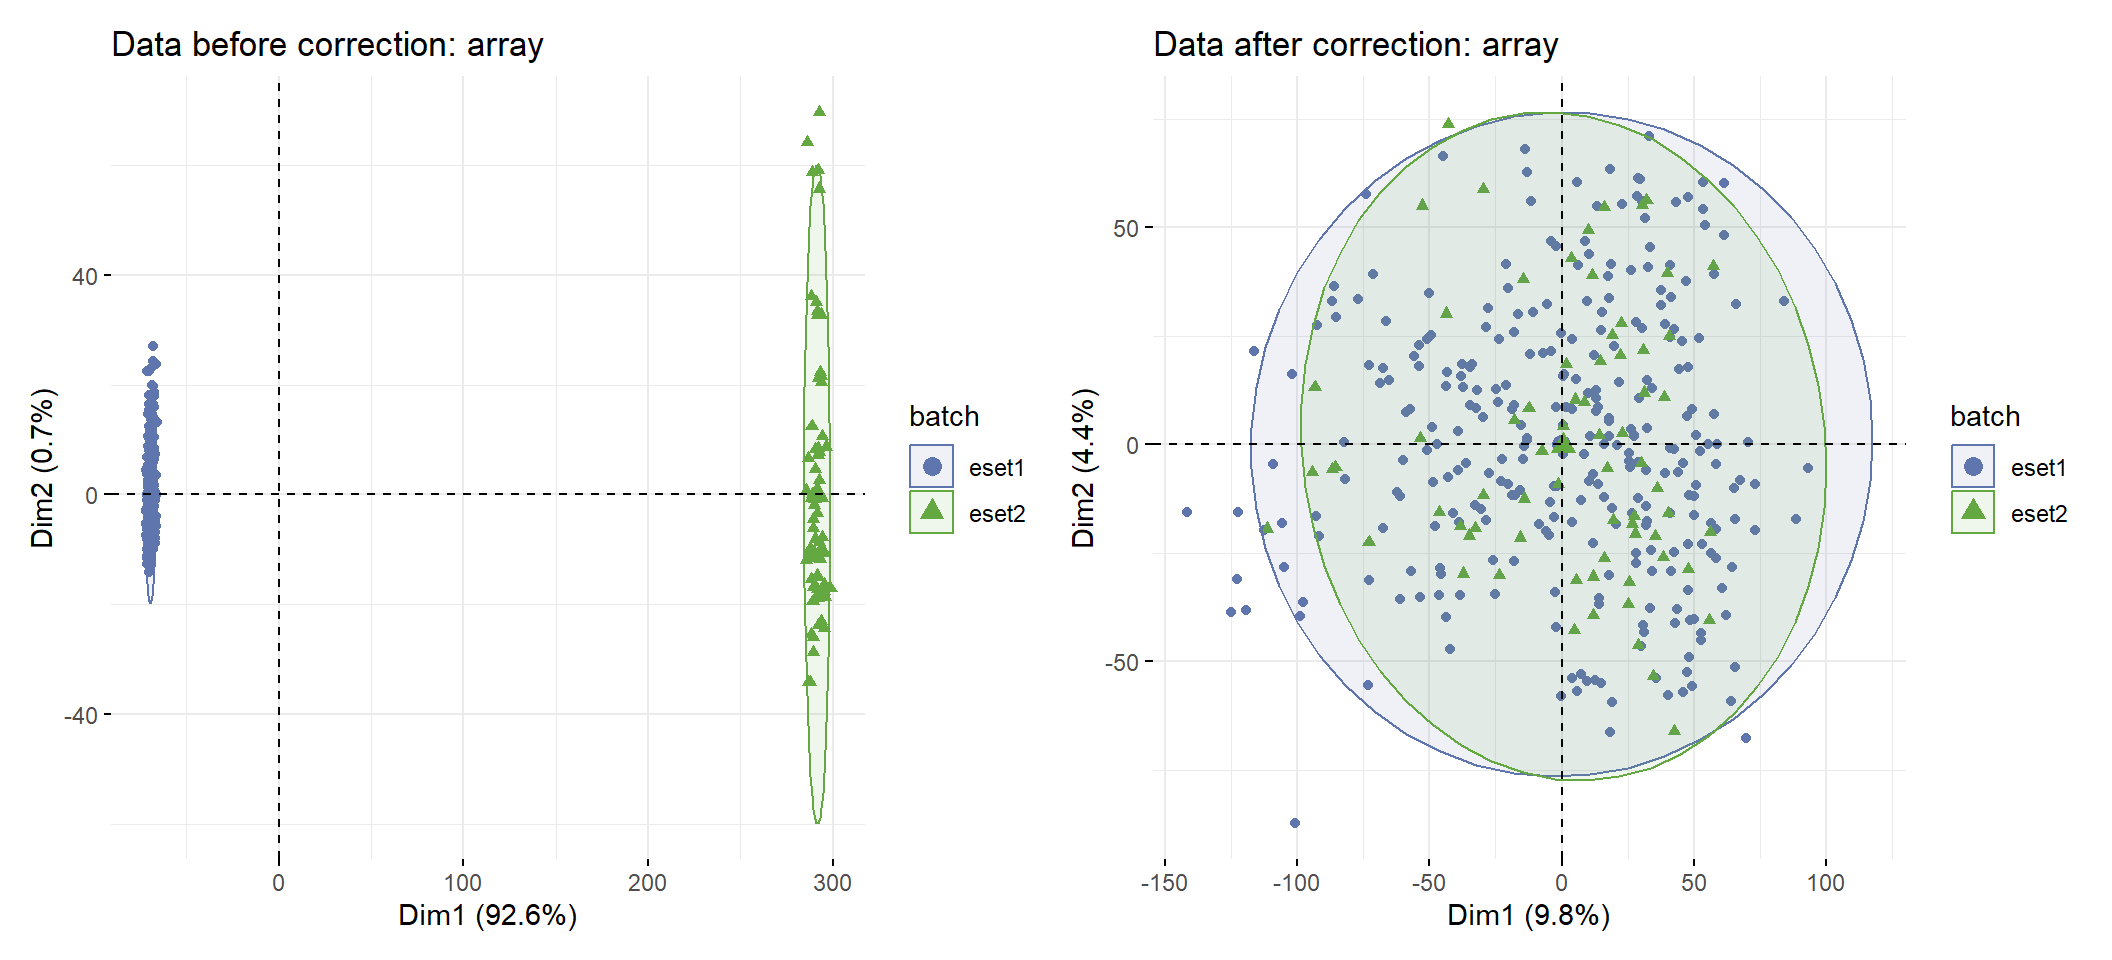
\includegraphics{signature-analysis_files/figure-latex/unnamed-chunk-14-1} \end{center}

\hypertarget{focus-on-target-signatures}{%
\section{Focus on target signatures}\label{focus-on-target-signatures}}

\begin{Shaded}
\begin{Highlighting}[]
\NormalTok{p1 }\OtherTok{\textless{}{-}} \FunctionTok{sig\_box}\NormalTok{(}\AttributeTok{data           =}\NormalTok{ input, }
              \AttributeTok{signature      =} \StringTok{"Glycogen\_Biosynthesis"}\NormalTok{,}
              \AttributeTok{variable       =} \StringTok{"Subtype"}\NormalTok{,}
              \AttributeTok{jitter         =} \ConstantTok{FALSE}\NormalTok{,}
              \AttributeTok{cols           =}  \ConstantTok{NULL}\NormalTok{,}
              \AttributeTok{palette        =} \StringTok{"jama"}\NormalTok{,}
              \AttributeTok{show\_pvalue    =} \ConstantTok{TRUE}\NormalTok{,}
              \AttributeTok{size\_of\_pvalue =} \DecValTok{5}\NormalTok{,}
              \AttributeTok{hjust          =} \DecValTok{1}\NormalTok{, }
              \AttributeTok{angle\_x\_text   =} \DecValTok{60}\NormalTok{, }
              \AttributeTok{size\_of\_font   =} \DecValTok{8}\NormalTok{)}
\end{Highlighting}
\end{Shaded}

\begin{verbatim}
## # A tibble: 6 x 8
##   .y.       group1    group2           p    p.adj p.format p.signif method  
##   <chr>     <chr>     <chr>        <dbl>    <dbl> <chr>    <chr>    <chr>   
## 1 signature EMT       MSI       5.39e-15 3.20e-14 5.4e-15  ****     Wilcoxon
## 2 signature EMT       MSS/TP53- 5.53e-13 2.8 e-12 5.5e-13  ****     Wilcoxon
## 3 signature EMT       MSS/TP53+ 1.90e-12 7.6 e-12 1.9e-12  ****     Wilcoxon
## 4 signature MSI       MSS/TP53- 1.14e- 3 3.4 e- 3 0.0011   **       Wilcoxon
## 5 signature MSI       MSS/TP53+ 7.05e- 3 1.4 e- 2 0.0071   **       Wilcoxon
## 6 signature MSS/TP53- MSS/TP53+ 7.16e- 1 7.2 e- 1 0.7161   ns       Wilcoxon
\end{verbatim}

\begin{Shaded}
\begin{Highlighting}[]
\NormalTok{p2 }\OtherTok{\textless{}{-}} \FunctionTok{sig\_box}\NormalTok{(}\AttributeTok{data           =}\NormalTok{ input, }
              \AttributeTok{signature      =} \StringTok{"Pan\_F\_TBRs"}\NormalTok{,}
              \AttributeTok{variable       =} \StringTok{"Subtype"}\NormalTok{,}
              \AttributeTok{jitter         =} \ConstantTok{FALSE}\NormalTok{,}
              \AttributeTok{cols           =} \ConstantTok{NULL}\NormalTok{,}
              \AttributeTok{palette        =} \StringTok{"jama"}\NormalTok{,}
              \AttributeTok{show\_pvalue    =} \ConstantTok{TRUE}\NormalTok{,}
              \AttributeTok{angle\_x\_text   =} \DecValTok{60}\NormalTok{, }
              \AttributeTok{hjust          =} \DecValTok{1}\NormalTok{, }
              \AttributeTok{size\_of\_pvalue =} \DecValTok{5}\NormalTok{, }
              \AttributeTok{size\_of\_font   =} \DecValTok{8}\NormalTok{)}
\end{Highlighting}
\end{Shaded}

\begin{verbatim}
## # A tibble: 6 x 8
##   .y.       group1    group2           p    p.adj p.format p.signif method  
##   <chr>     <chr>     <chr>        <dbl>    <dbl> <chr>    <chr>    <chr>   
## 1 signature EMT       MSI       7.98e-17 3.20e-16 <2e-16   ****     Wilcoxon
## 2 signature EMT       MSS/TP53- 1.70e-17 1   e-16 <2e-16   ****     Wilcoxon
## 3 signature EMT       MSS/TP53+ 2.57e-17 1.3 e-16 <2e-16   ****     Wilcoxon
## 4 signature MSI       MSS/TP53- 1.32e- 2 4   e- 2 0.013    *        Wilcoxon
## 5 signature MSI       MSS/TP53+ 6.99e- 2 1.4 e- 1 0.070    ns       Wilcoxon
## 6 signature MSS/TP53- MSS/TP53+ 4.02e- 1 4   e- 1 0.402    ns       Wilcoxon
\end{verbatim}

\begin{Shaded}
\begin{Highlighting}[]
\NormalTok{p3 }\OtherTok{\textless{}{-}} \FunctionTok{sig\_box}\NormalTok{(}\AttributeTok{data           =}\NormalTok{ input, }
              \AttributeTok{signature      =} \StringTok{"Immune\_Checkpoint"}\NormalTok{,}
              \AttributeTok{variable       =} \StringTok{"Subtype"}\NormalTok{,}
              \AttributeTok{jitter          =} \ConstantTok{TRUE}\NormalTok{,}
              \AttributeTok{cols           =} \ConstantTok{NULL}\NormalTok{,}
              \AttributeTok{palette        =} \StringTok{"jama"}\NormalTok{,}
              \AttributeTok{show\_pvalue    =} \ConstantTok{TRUE}\NormalTok{,}
              \AttributeTok{angle\_x\_text   =} \DecValTok{60}\NormalTok{, }
              \AttributeTok{hjust          =} \DecValTok{1}\NormalTok{, }
              \AttributeTok{size\_of\_pvalue =} \DecValTok{5}\NormalTok{, }
              \AttributeTok{size\_of\_font   =} \DecValTok{8}\NormalTok{)}
\end{Highlighting}
\end{Shaded}

\begin{verbatim}
## # A tibble: 6 x 8
##   .y.       group1    group2           p        p.adj p.format p.signif method  
##   <chr>     <chr>     <chr>        <dbl>        <dbl> <chr>    <chr>    <chr>   
## 1 signature EMT       MSI       2.20e- 2 0.044        0.0220   *        Wilcoxon
## 2 signature EMT       MSS/TP53- 2.11e- 3 0.0085       0.0021   **       Wilcoxon
## 3 signature EMT       MSS/TP53+ 4.03e- 1 0.4          0.4026   ns       Wilcoxon
## 4 signature MSI       MSS/TP53- 9.13e-10 0.0000000055 9.1e-10  ****     Wilcoxon
## 5 signature MSI       MSS/TP53+ 5.03e- 4 0.0025       0.0005   ***      Wilcoxon
## 6 signature MSS/TP53- MSS/TP53+ 4.82e- 3 0.014        0.0048   **       Wilcoxon
\end{verbatim}

\begin{Shaded}
\begin{Highlighting}[]
\NormalTok{p1}\SpecialCharTok{|}\NormalTok{p2}\SpecialCharTok{|}\NormalTok{p3}
\end{Highlighting}
\end{Shaded}

\begin{center}\includegraphics{signature-analysis_files/figure-latex/unnamed-chunk-16-1} \end{center}

\hypertarget{survival-analysis}{%
\section{Survival analysis}\label{survival-analysis}}

Signature的多种分层下的生存分析

\begin{Shaded}
\begin{Highlighting}[]
\NormalTok{res }\OtherTok{\textless{}{-}}       \FunctionTok{sig\_surv\_plot}\NormalTok{(}\AttributeTok{input\_pdata       =}\NormalTok{ input, }
                           \AttributeTok{signature         =} \StringTok{"Glycogen\_Biosynthesis"}\NormalTok{,}
                           \AttributeTok{cols              =} \ConstantTok{NULL}\NormalTok{, }
                           \AttributeTok{palette           =} \StringTok{"jco"}\NormalTok{,}
                           \AttributeTok{project           =} \StringTok{"ACRG"}\NormalTok{,}
                           \AttributeTok{time              =} \StringTok{"OS\_time"}\NormalTok{,}
                           \AttributeTok{status            =} \StringTok{"OS\_status"}\NormalTok{,}
                           \AttributeTok{time\_type         =} \StringTok{"month"}\NormalTok{,}
                           \AttributeTok{save\_path         =} \StringTok{"result"}\NormalTok{)}
\end{Highlighting}
\end{Shaded}

\begin{verbatim}
##           ID   time status Glycogen_Biosynthesis group3 group2 bestcutoff
## 1 GSM1523727  88.73      0            -0.3612213 Middle    Low        Low
## 2 GSM1523728  88.23      0            -0.6926726    Low    Low        Low
## 3 GSM1523729  88.23      0            -0.9388531    Low    Low        Low
## 4 GSM1523744 105.70      0            -1.1825136    Low    Low        Low
## 5 GSM1523745 105.53      0            -0.3034304 Middle    Low        Low
## 6 GSM1523746  25.50      1             0.7517934   High   High       High
\end{verbatim}

\begin{verbatim}
## [1] ">>>>>>>>>"
\end{verbatim}

\begin{Shaded}
\begin{Highlighting}[]
\NormalTok{res}\SpecialCharTok{$}\NormalTok{plots}
\end{Highlighting}
\end{Shaded}

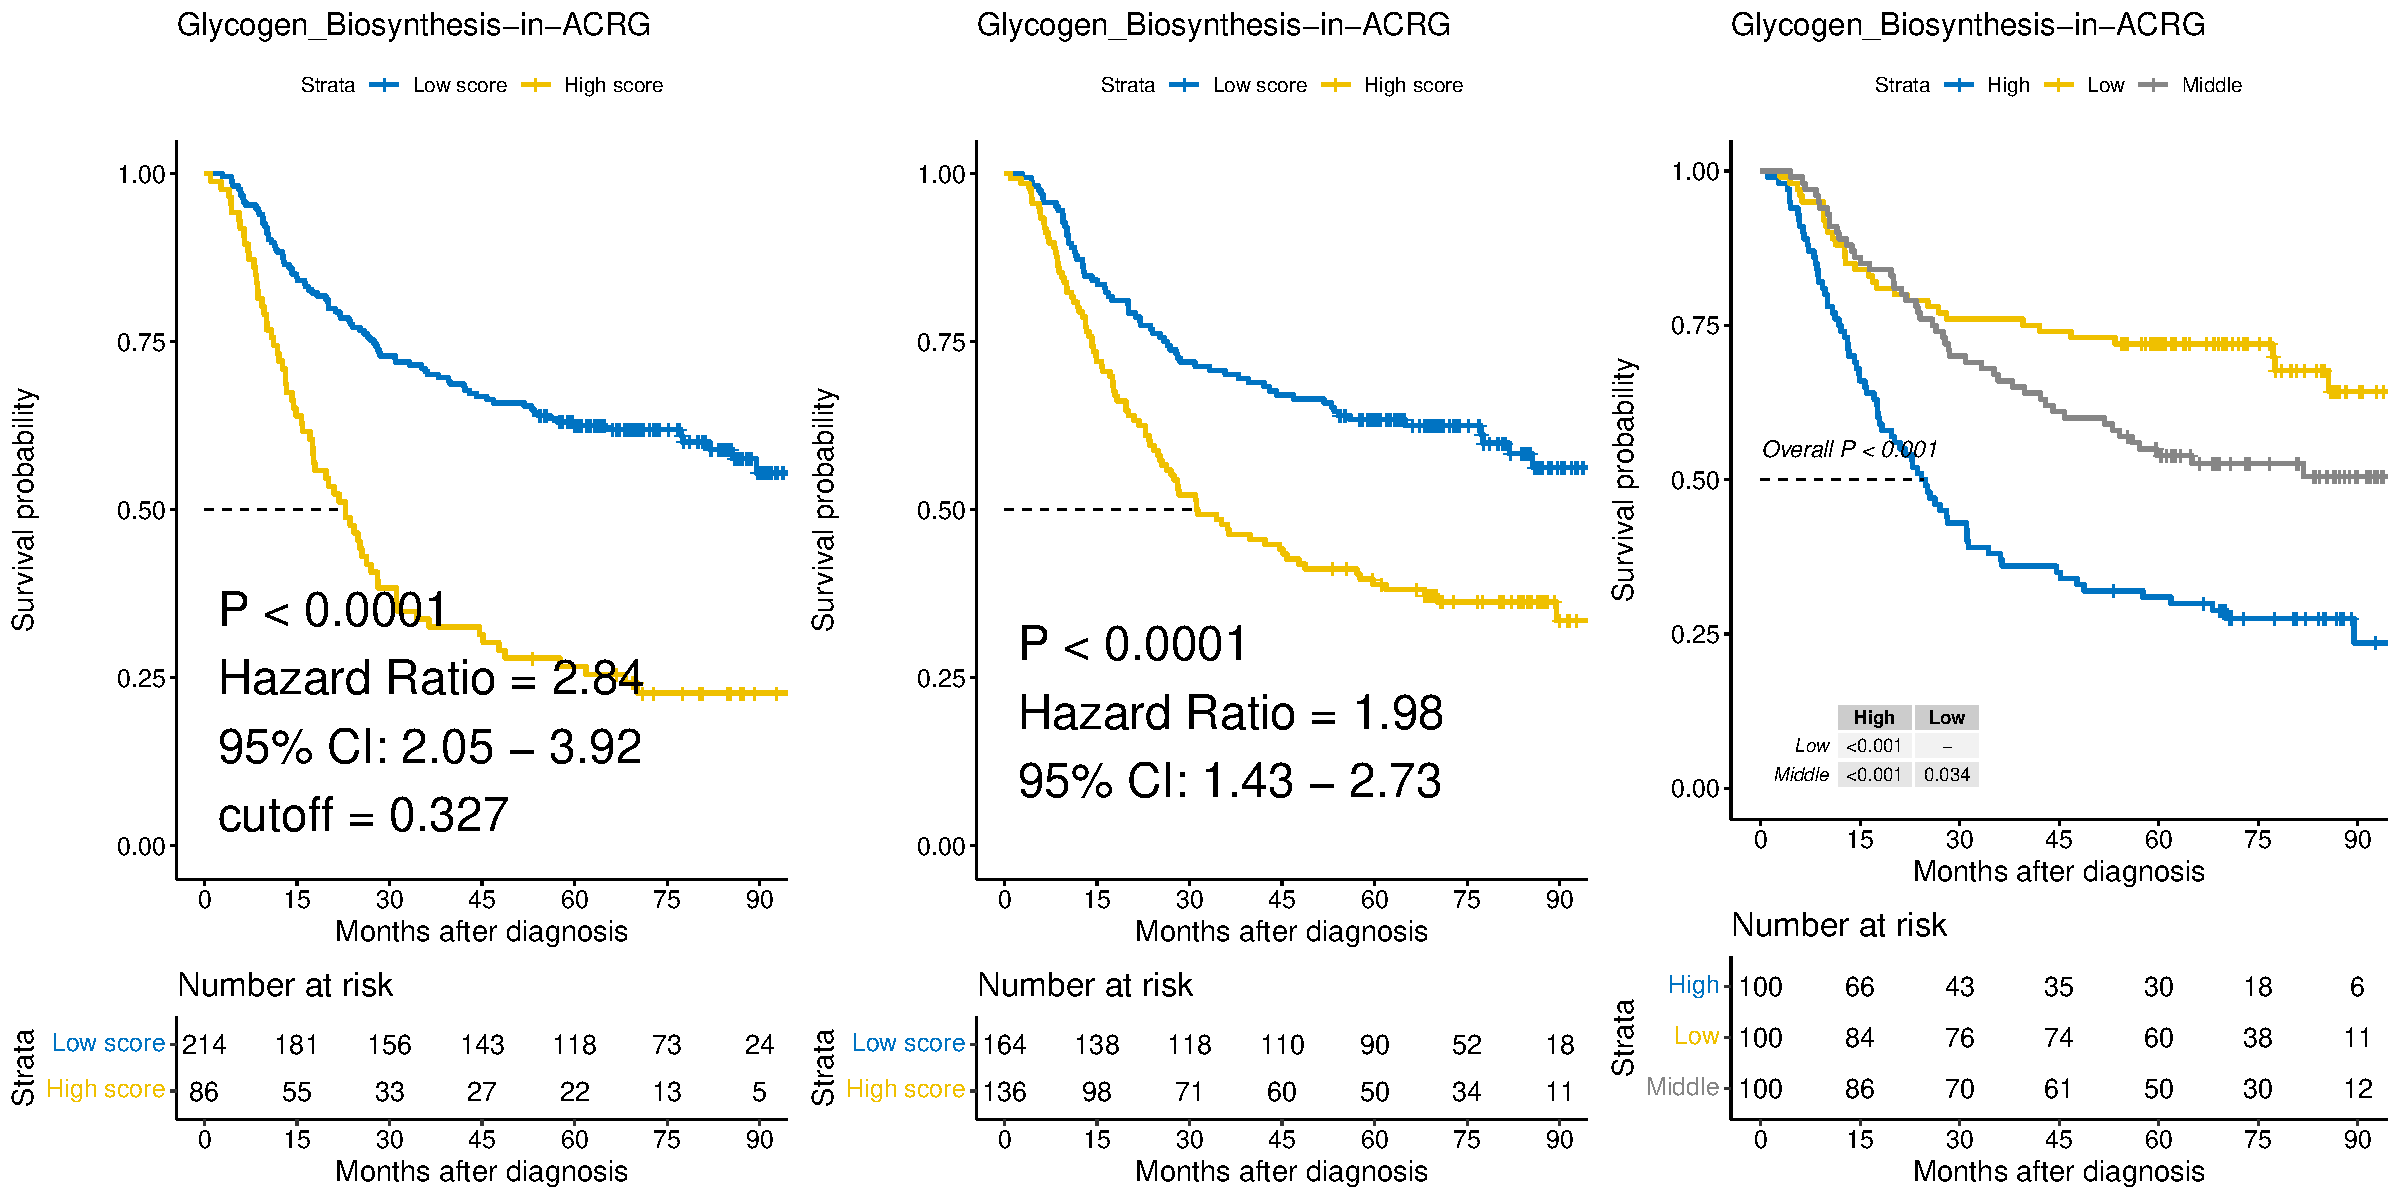
\includegraphics{signature-analysis_files/figure-latex/unnamed-chunk-17-1.pdf}

Signature在预测生存上的ROC

\begin{Shaded}
\begin{Highlighting}[]
\NormalTok{p1}\OtherTok{\textless{}{-}} \FunctionTok{roc\_time}\NormalTok{(}\AttributeTok{input      =}\NormalTok{ input,  }
             \AttributeTok{vars       =} \StringTok{"Glycogen\_Biosynthesis"}\NormalTok{, }
             \AttributeTok{time       =} \StringTok{"OS\_time"}\NormalTok{,}
             \AttributeTok{status     =} \StringTok{"OS\_status"}\NormalTok{, }
             \AttributeTok{time\_point =} \FunctionTok{c}\NormalTok{(}\DecValTok{12}\NormalTok{, }\DecValTok{24}\NormalTok{, }\DecValTok{36}\NormalTok{), }
             \AttributeTok{time\_type  =} \StringTok{"month"}\NormalTok{,}
             \AttributeTok{palette    =} \StringTok{"jama"}\NormalTok{,}
             \AttributeTok{cols       =} \StringTok{"normal"}\NormalTok{,}
             \AttributeTok{seed       =} \DecValTok{1234}\NormalTok{, }
             \AttributeTok{show\_col   =} \ConstantTok{FALSE}\NormalTok{, }
             \AttributeTok{path       =} \StringTok{"result"}\NormalTok{, }
             \AttributeTok{main       =} \StringTok{"OS"}\NormalTok{,}
             \AttributeTok{index      =} \DecValTok{1}\NormalTok{,}
             \AttributeTok{fig.type   =} \StringTok{"pdf"}\NormalTok{,}
             \AttributeTok{width      =} \DecValTok{5}\NormalTok{,}
             \AttributeTok{height     =} \FloatTok{5.2}\NormalTok{)}
\end{Highlighting}
\end{Shaded}

\begin{verbatim}
## [1] ">>>-- Range of Time: "
## [1]   1.0 105.7
\end{verbatim}

\begin{Shaded}
\begin{Highlighting}[]
\NormalTok{p2}\OtherTok{\textless{}{-}} \FunctionTok{roc\_time}\NormalTok{(}\AttributeTok{input      =}\NormalTok{ input,  }
             \AttributeTok{vars       =} \StringTok{"Glycogen\_Biosynthesis"}\NormalTok{, }
             \AttributeTok{time       =} \StringTok{"RFS\_time"}\NormalTok{,}
             \AttributeTok{status     =} \StringTok{"RFS\_status"}\NormalTok{, }
             \AttributeTok{time\_point =} \FunctionTok{c}\NormalTok{(}\DecValTok{12}\NormalTok{, }\DecValTok{24}\NormalTok{, }\DecValTok{36}\NormalTok{), }
             \AttributeTok{time\_type  =} \StringTok{"month"}\NormalTok{,}
             \AttributeTok{palette    =} \StringTok{"jama"}\NormalTok{,}
             \AttributeTok{cols       =} \StringTok{"normal"}\NormalTok{,}
             \AttributeTok{seed       =} \DecValTok{1234}\NormalTok{, }
             \AttributeTok{show\_col   =} \ConstantTok{FALSE}\NormalTok{, }
             \AttributeTok{path       =} \StringTok{"result"}\NormalTok{, }
             \AttributeTok{main       =} \StringTok{"OS"}\NormalTok{,}
             \AttributeTok{index      =} \DecValTok{1}\NormalTok{,}
             \AttributeTok{fig.type   =} \StringTok{"pdf"}\NormalTok{,}
             \AttributeTok{width      =} \DecValTok{5}\NormalTok{,}
             \AttributeTok{height     =} \FloatTok{5.2}\NormalTok{)}
\end{Highlighting}
\end{Shaded}

\begin{verbatim}
## [1] ">>>-- Range of Time: "
## [1]   0.10 100.87
\end{verbatim}

\begin{Shaded}
\begin{Highlighting}[]
\NormalTok{p1}\SpecialCharTok{|}\NormalTok{p2}
\end{Highlighting}
\end{Shaded}

\includegraphics{signature-analysis_files/figure-latex/unnamed-chunk-18-1.pdf}

\hypertarget{batch-correlation-analysis}{%
\section{Batch correlation analysis}\label{batch-correlation-analysis}}

寻找与目标signature相关的基因或者signatures

\begin{Shaded}
\begin{Highlighting}[]
\NormalTok{res }\OtherTok{\textless{}{-}} \FunctionTok{batch\_cor}\NormalTok{(}\AttributeTok{data =}\NormalTok{ input, }\AttributeTok{target =} \StringTok{"Glycogen\_Biosynthesis"}\NormalTok{, }\AttributeTok{feature =} \FunctionTok{colnames}\NormalTok{(input)[}\DecValTok{69}\SpecialCharTok{:}\FunctionTok{ncol}\NormalTok{(input)])}
\FunctionTok{head}\NormalTok{(res)}
\end{Highlighting}
\end{Shaded}

\begin{verbatim}
## # A tibble: 6 x 6
##   sig_names                         p.value statistic    p.adj log10pvalue stars
##   <chr>                               <dbl>     <dbl>    <dbl>       <dbl> <fct>
## 1 TMEscoreB_CIR                    8.89e-42     0.678 2.27e-39        41.1 **** 
## 2 Glycine__Serine_and_Threonine_M~ 7.49e-40    -0.666 9.54e-38        39.1 **** 
## 3 Ether_Lipid_Metabolism           3.84e-39     0.662 3.27e-37        38.4 **** 
## 4 MDSC_Peng_et_al                  1.13e-38     0.659 7.21e-37        37.9 **** 
## 5 Glycerophospholipid_Metabolism   8.72e-38    -0.653 4.44e-36        37.1 **** 
## 6 TIP_Release_of_cancer_cell_anti~ 2.32e-37    -0.650 9.86e-36        36.6 ****
\end{verbatim}

\begin{Shaded}
\begin{Highlighting}[]
\NormalTok{p1}\OtherTok{\textless{}{-}} \FunctionTok{get\_cor}\NormalTok{(}\AttributeTok{eset =}\NormalTok{ sig\_tme, }\AttributeTok{pdata =}\NormalTok{ pdata\_acrg, }\AttributeTok{var1 =} \StringTok{"Glycogen\_Biosynthesis"}\NormalTok{, }\AttributeTok{var2 =} \StringTok{"TMEscore\_CIR"}\NormalTok{, }\AttributeTok{subtype =} \StringTok{"Subtype"}\NormalTok{, }\AttributeTok{palette =} \StringTok{"aaas"}\NormalTok{)}
\end{Highlighting}
\end{Shaded}

\begin{verbatim}
## 
##  Spearman's rank correlation rho
## 
## data:  data[, var1] and data[, var2]
## S = 7282858, p-value < 2.2e-16
## alternative hypothesis: true rho is not equal to 0
## sample estimates:
##        rho 
## -0.6184309 
## 
## [1] ">>>--- The exact p value is: 4.78971420439895e-33"
##       EMT       MSI MSS/TP53- MSS/TP53+ 
##        46        68       107        79
\end{verbatim}

\begin{Shaded}
\begin{Highlighting}[]
\NormalTok{p2}\OtherTok{\textless{}{-}} \FunctionTok{get\_cor}\NormalTok{(}\AttributeTok{eset =}\NormalTok{ sig\_tme, }\AttributeTok{pdata =}\NormalTok{ pdata\_acrg, }\AttributeTok{var1 =} \StringTok{"Glycogen\_Biosynthesis"}\NormalTok{, }\AttributeTok{var2 =} \StringTok{"TGFb.myCAF"}\NormalTok{, }\AttributeTok{subtype =} \StringTok{"Subtype"}\NormalTok{, }\AttributeTok{palette =} \StringTok{"aaas"}\NormalTok{)}
\end{Highlighting}
\end{Shaded}

\begin{verbatim}
## 
##  Spearman's rank correlation rho
## 
## data:  data[, var1] and data[, var2]
## S = 2471758, p-value < 2.2e-16
## alternative hypothesis: true rho is not equal to 0
## sample estimates:
##       rho 
## 0.4507143 
## 
## [1] ">>>--- The exact p value is: 2.04505761057615e-16"
##       EMT       MSI MSS/TP53- MSS/TP53+ 
##        46        68       107        79
\end{verbatim}

\begin{Shaded}
\begin{Highlighting}[]
\NormalTok{p1}\SpecialCharTok{|}\NormalTok{p2}
\end{Highlighting}
\end{Shaded}

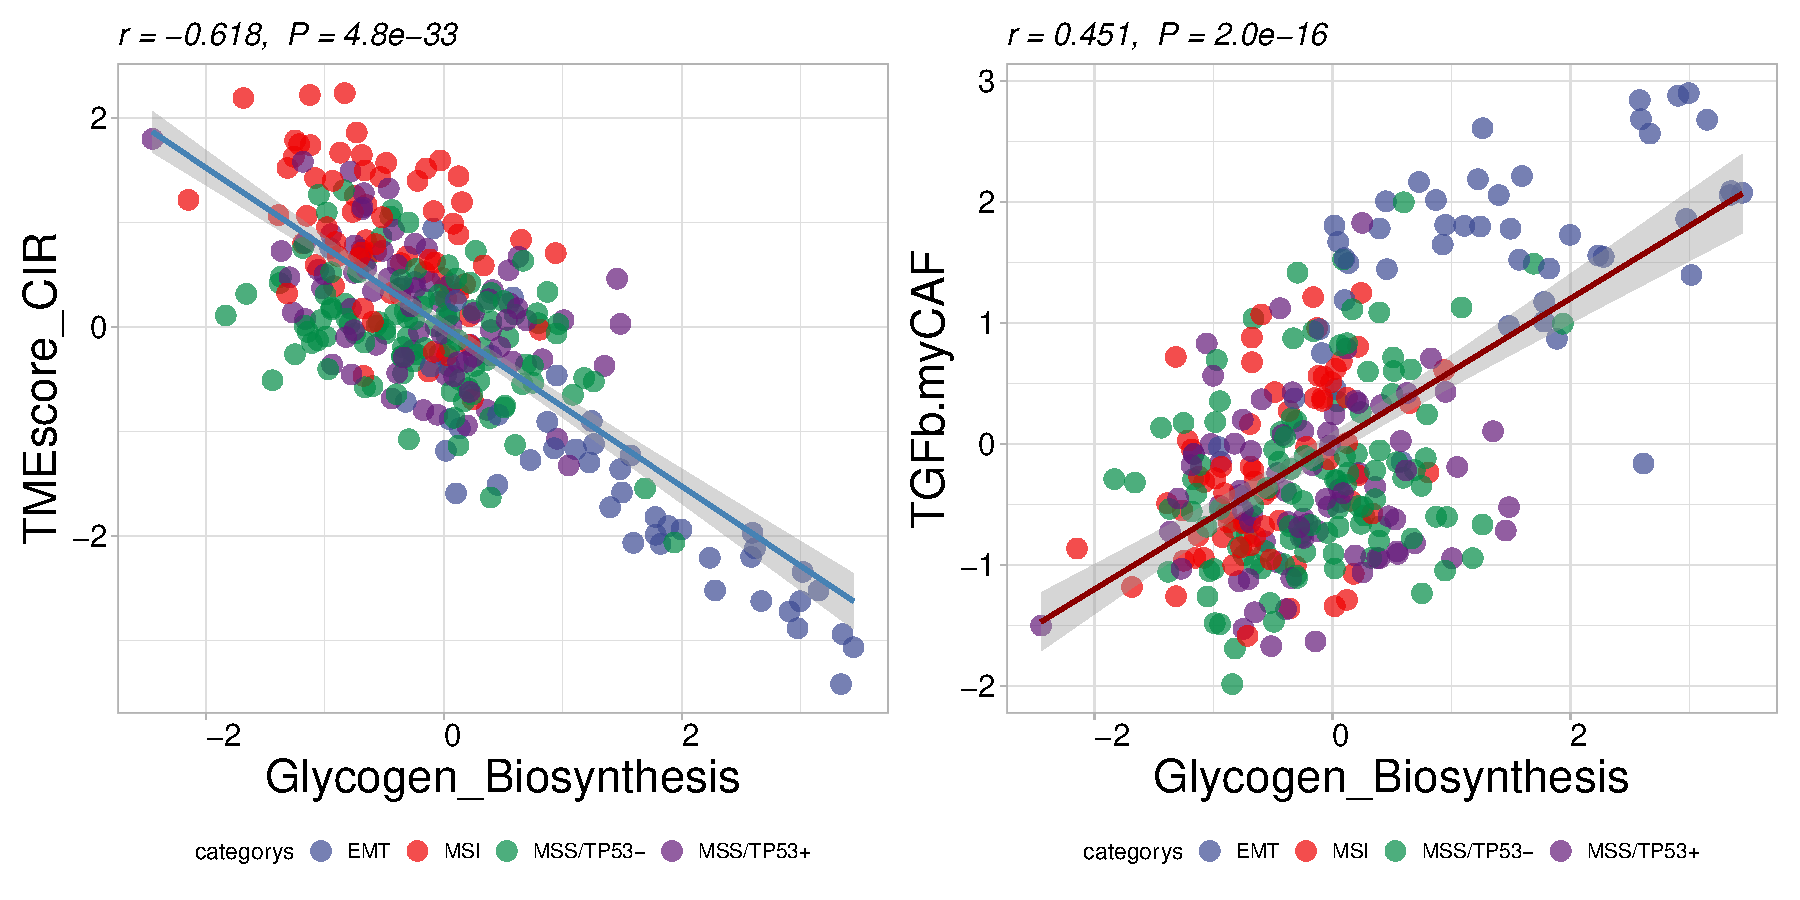
\includegraphics{signature-analysis_files/figure-latex/unnamed-chunk-21-1.pdf}

\begin{Shaded}
\begin{Highlighting}[]
\NormalTok{feas1 }\OtherTok{\textless{}{-}} \FunctionTok{c}\NormalTok{(}\StringTok{"Glycogen\_Biosynthesis"}\NormalTok{, }\StringTok{"Ferroptosis"}\NormalTok{)}
\NormalTok{feas2 }\OtherTok{\textless{}{-}} \FunctionTok{c}\NormalTok{(}\StringTok{"Glutathione\_Metabolism"}\NormalTok{, }\StringTok{"TMEscore\_CIR"}\NormalTok{, }\StringTok{"Purine\_Metabolism"}\NormalTok{, }\StringTok{"ICB\_resistance\_Peng\_et\_al"}\NormalTok{, }\StringTok{"Interleukins\_Li\_et\_al"}\NormalTok{, }\StringTok{"TLS\_Nature"}\NormalTok{)}
\NormalTok{p }\OtherTok{\textless{}{-}} \FunctionTok{get\_cor\_matrix}\NormalTok{(}\AttributeTok{data           =}\NormalTok{ input, }
                    \AttributeTok{feas1          =}\NormalTok{ feas2, }
                    \AttributeTok{feas2          =}\NormalTok{ feas1,}
                    \AttributeTok{method         =} \StringTok{"pearson"}\NormalTok{,}
                    \AttributeTok{font.size.star =} \DecValTok{8}\NormalTok{, }
                    \AttributeTok{font.size      =} \DecValTok{15}\NormalTok{, }
                    \AttributeTok{fill\_by\_cor    =} \ConstantTok{FALSE}\NormalTok{, }
                    \AttributeTok{round.num      =} \DecValTok{1}\NormalTok{)}
\end{Highlighting}
\end{Shaded}

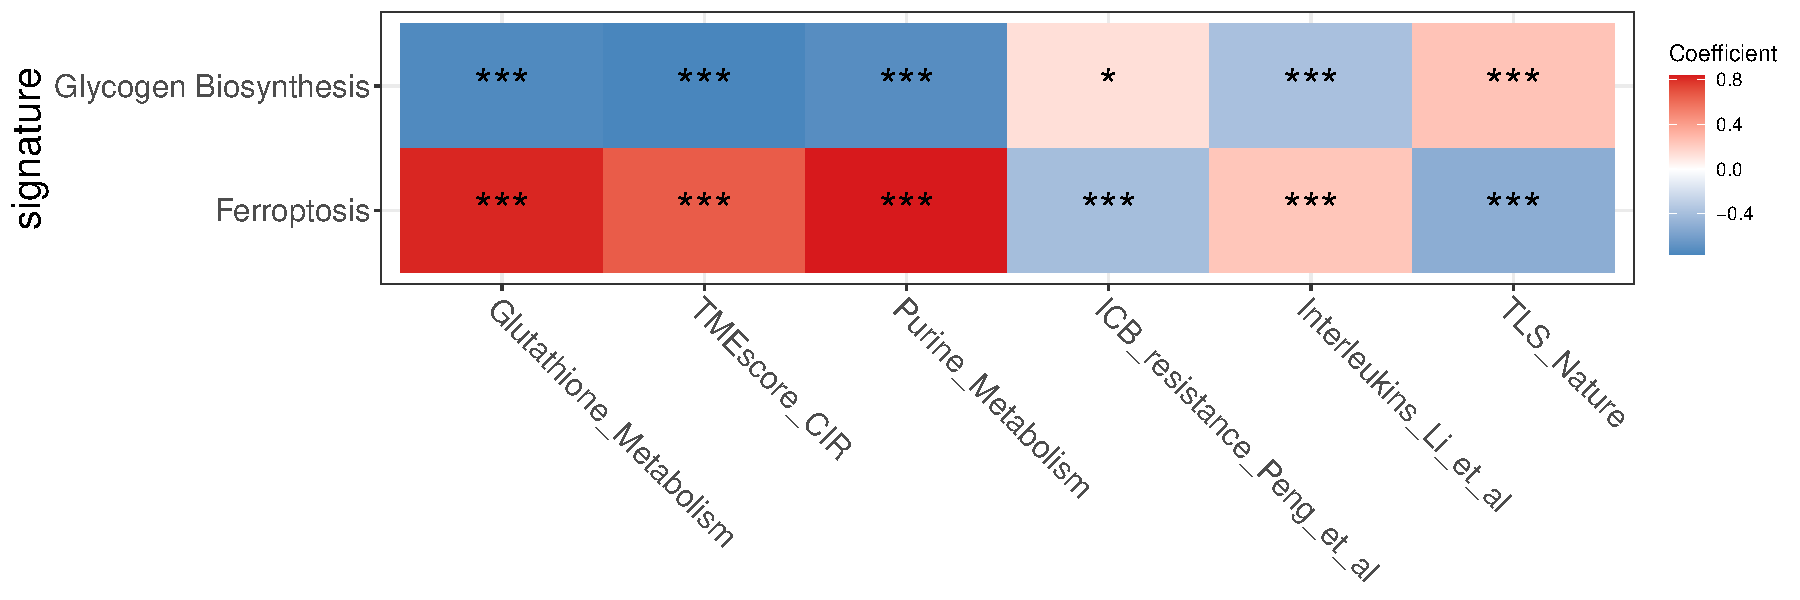
\includegraphics{signature-analysis_files/figure-latex/unnamed-chunk-22-1.pdf}

\hypertarget{visulization-of-correlations}{%
\section{Visulization of correlations}\label{visulization-of-correlations}}

\begin{Shaded}
\begin{Highlighting}[]
\NormalTok{input2 }\OtherTok{\textless{}{-}} \FunctionTok{combine\_pd\_eset}\NormalTok{(}\AttributeTok{eset =}\NormalTok{ eset, }\AttributeTok{pdata =}\NormalTok{  input[, }\FunctionTok{c}\NormalTok{(}\StringTok{"ID"}\NormalTok{, }\StringTok{"Glycogen\_Biosynthesis"}\NormalTok{, }\StringTok{"TLS\_Nature"}\NormalTok{, }\StringTok{"Ferroptosis"}\NormalTok{)])}
\NormalTok{feas1 }\OtherTok{\textless{}{-}} \FunctionTok{c}\NormalTok{(}\StringTok{"Glycogen\_Biosynthesis"}\NormalTok{,}\StringTok{"TLS\_Nature"}\NormalTok{, }\StringTok{"Ferroptosis"}\NormalTok{)}
\NormalTok{feas2 }\OtherTok{\textless{}{-}}\NormalTok{ signature\_collection}\SpecialCharTok{$}\NormalTok{CD\_8\_T\_effector}
\NormalTok{feas2}
\end{Highlighting}
\end{Shaded}

\begin{verbatim}
## [1] "CD8A"   "GZMA"   "GZMB"   "IFNG"   "CXCL9"  "CXCL10" "PRF1"   "TBX21"
\end{verbatim}

\begin{Shaded}
\begin{Highlighting}[]
\NormalTok{p }\OtherTok{\textless{}{-}} \FunctionTok{get\_cor\_matrix}\NormalTok{(}\AttributeTok{data           =}\NormalTok{ input2, }
                    \AttributeTok{feas1          =}\NormalTok{ feas2, }
                    \AttributeTok{feas2          =}\NormalTok{ feas1,}
                    \AttributeTok{method         =} \StringTok{"pearson"}\NormalTok{,}
                    \AttributeTok{scale          =}\NormalTok{ T, }
                    \AttributeTok{font.size.star =} \DecValTok{8}\NormalTok{, }
                    \AttributeTok{font.size      =} \DecValTok{15}\NormalTok{, }
                    \AttributeTok{fill\_by\_cor    =} \ConstantTok{FALSE}\NormalTok{, }
                    \AttributeTok{round.num      =} \DecValTok{1}\NormalTok{)}
\end{Highlighting}
\end{Shaded}

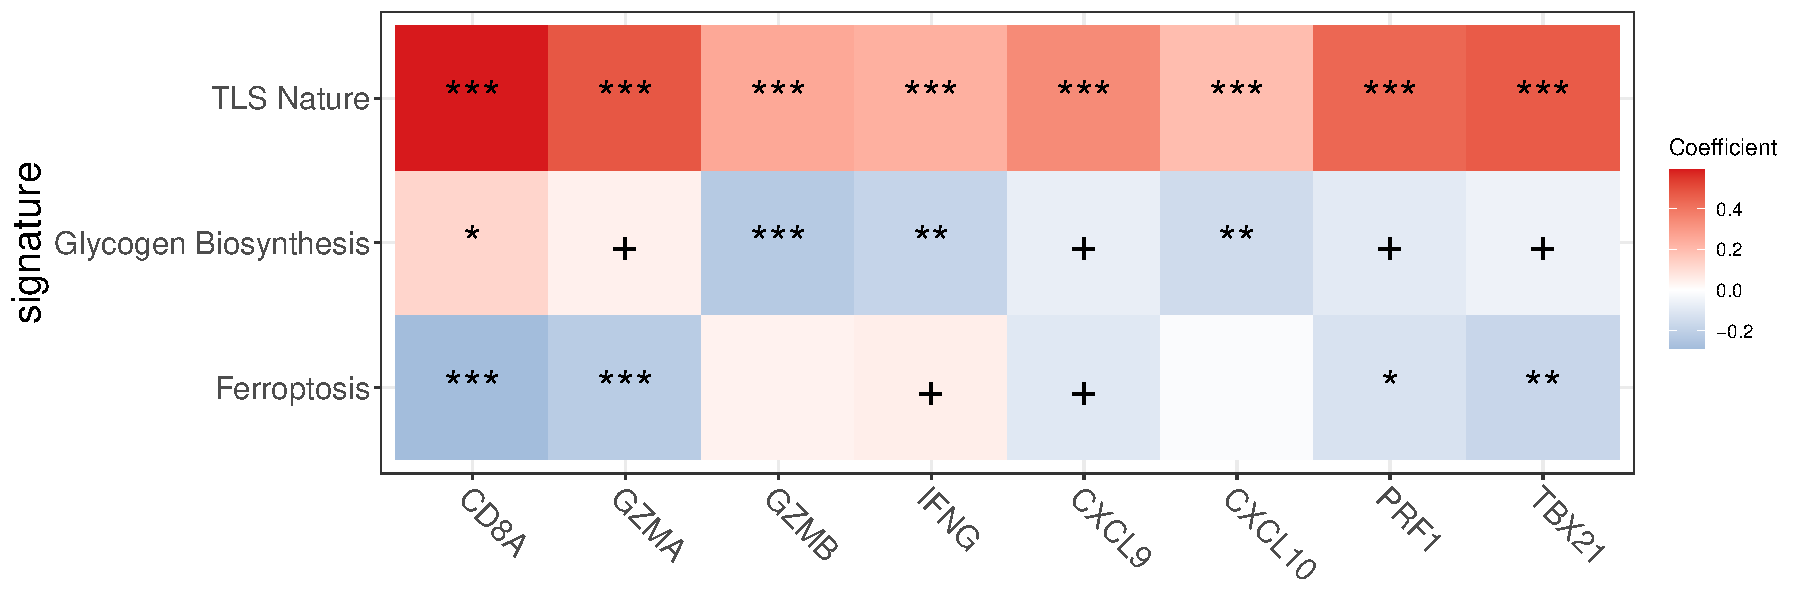
\includegraphics{signature-analysis_files/figure-latex/unnamed-chunk-23-1.pdf}

\begin{Shaded}
\begin{Highlighting}[]
\NormalTok{p }\OtherTok{\textless{}{-}} \FunctionTok{get\_cor\_matrix}\NormalTok{(}\AttributeTok{data           =}\NormalTok{ input2, }
                    \AttributeTok{feas1          =}\NormalTok{ feas2, }
                    \AttributeTok{feas2          =}\NormalTok{ feas1,}
                    \AttributeTok{method         =} \StringTok{"pearson"}\NormalTok{,}
                    \AttributeTok{scale          =}\NormalTok{ T, }
                    \AttributeTok{font.size.star =} \DecValTok{8}\NormalTok{, }
                    \AttributeTok{font.size      =} \DecValTok{15}\NormalTok{, }
                    \AttributeTok{fill\_by\_cor    =} \ConstantTok{TRUE}\NormalTok{, }
                    \AttributeTok{round.num      =} \DecValTok{2}\NormalTok{)}
\end{Highlighting}
\end{Shaded}

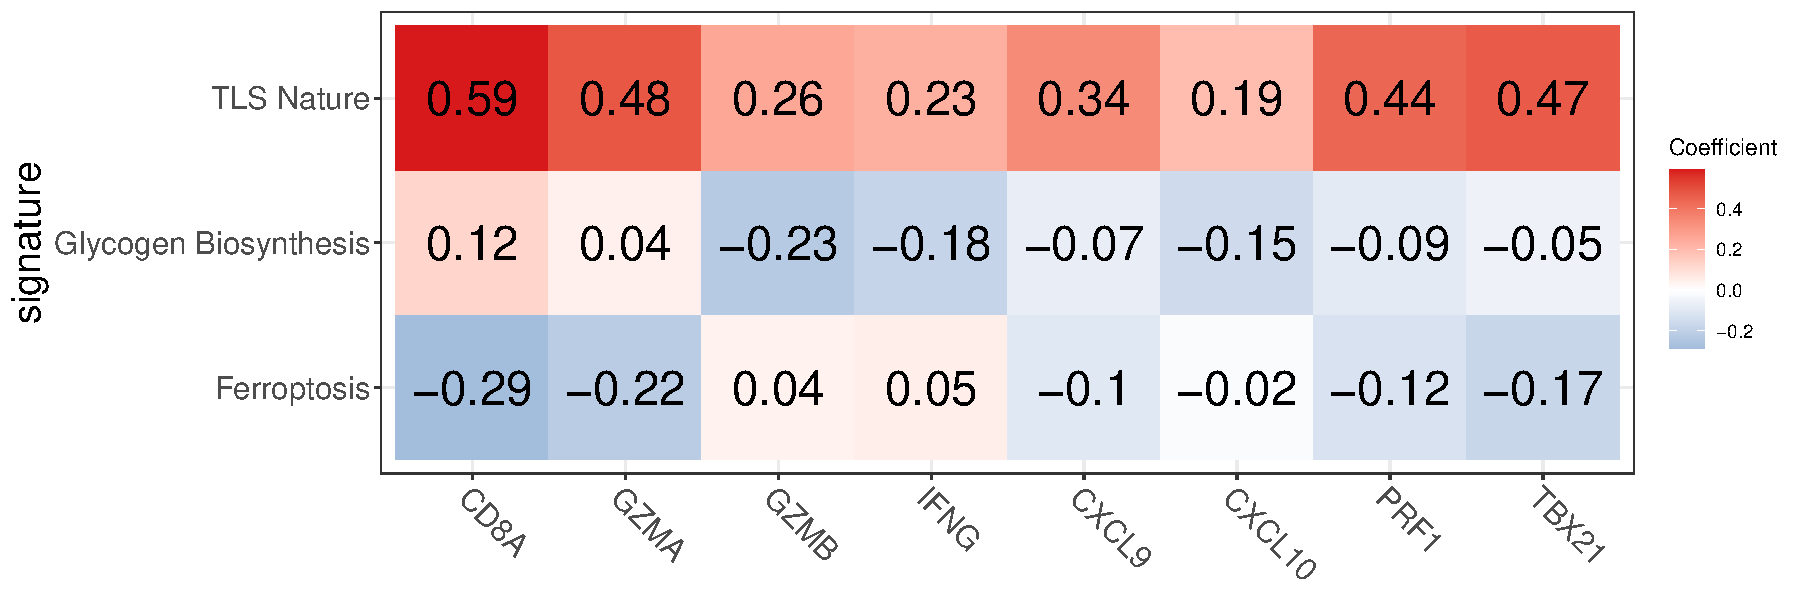
\includegraphics{signature-analysis_files/figure-latex/unnamed-chunk-24-1.pdf}

\hypertarget{tme-deconvolution}{%
\chapter{\texorpdfstring{\textbf{TME deconvolution}}{TME deconvolution}}\label{tme-deconvolution}}

\hypertarget{loading-packages-3}{%
\section{Loading packages}\label{loading-packages-3}}

Load the IOBR package in your R session after the installation is complete:

\begin{Shaded}
\begin{Highlighting}[]
\FunctionTok{library}\NormalTok{(IOBR)}
\FunctionTok{library}\NormalTok{(survminer)}
\FunctionTok{library}\NormalTok{(tidyverse)}
\end{Highlighting}
\end{Shaded}

\hypertarget{downloading-data-for-example-3}{%
\section{Downloading data for example}\label{downloading-data-for-example-3}}

Obtaining data set from GEO \href{https://pubmed.ncbi.nlm.nih.gov/25894828/}{Gastric cancer: GSE62254} using \texttt{GEOquery} R package.

\begin{Shaded}
\begin{Highlighting}[]
\ControlFlowTok{if}\NormalTok{ (}\SpecialCharTok{!}\FunctionTok{requireNamespace}\NormalTok{(}\StringTok{"GEOquery"}\NormalTok{, }\AttributeTok{quietly =} \ConstantTok{TRUE}\NormalTok{))  BiocManager}\SpecialCharTok{::}\FunctionTok{install}\NormalTok{(}\StringTok{"GEOquery"}\NormalTok{)}
\FunctionTok{library}\NormalTok{(}\StringTok{"GEOquery"}\NormalTok{)}
\CommentTok{\# }\AlertTok{NOTE}\CommentTok{: This process may take a few minutes which depends on the internet connection speed. Please wait for its completion.}
\NormalTok{eset\_geo}\OtherTok{\textless{}{-}}\FunctionTok{getGEO}\NormalTok{(}\AttributeTok{GEO     =} \StringTok{"GSE62254"}\NormalTok{, }\AttributeTok{getGPL  =}\NormalTok{ F, }\AttributeTok{destdir =} \StringTok{"./"}\NormalTok{)}
\NormalTok{eset    }\OtherTok{\textless{}{-}}\NormalTok{eset\_geo[[}\DecValTok{1}\NormalTok{]]}
\NormalTok{eset    }\OtherTok{\textless{}{-}}\FunctionTok{exprs}\NormalTok{(eset)}
\NormalTok{eset[}\DecValTok{1}\SpecialCharTok{:}\DecValTok{5}\NormalTok{,}\DecValTok{1}\SpecialCharTok{:}\DecValTok{5}\NormalTok{]}
\end{Highlighting}
\end{Shaded}

\begin{verbatim}
##           GSM1523727 GSM1523728 GSM1523729 GSM1523744 GSM1523745
## 1007_s_at  3.2176645  3.0624323  3.0279131   2.921683  2.8456013
## 1053_at    2.4050109  2.4394879  2.2442708   2.345916  2.4328582
## 117_at     1.4933412  1.8067380  1.5959665   1.839822  1.8326058
## 121_at     2.1965561  2.2812181  2.1865556   2.258599  2.1874363
## 1255_g_at  0.8698382  0.9502466  0.8125414   1.012860  0.9441993
\end{verbatim}

Annotation of genes in the expression matrix and removal of duplicate genes.

\begin{Shaded}
\begin{Highlighting}[]
\FunctionTok{library}\NormalTok{(IOBR)}

\CommentTok{\# Load the annotation file \textasciigrave{}anno\_hug133plus2\textasciigrave{} in IOBR.}
\FunctionTok{head}\NormalTok{(anno\_hug133plus2)}
\end{Highlighting}
\end{Shaded}

\begin{verbatim}
## # A tibble: 6 x 2
##   probe_id  symbol 
##   <fct>     <fct>  
## 1 1007_s_at MIR4640
## 2 1053_at   RFC2   
## 3 117_at    HSPA6  
## 4 121_at    PAX8   
## 5 1255_g_at GUCA1A 
## 6 1294_at   MIR5193
\end{verbatim}

\begin{Shaded}
\begin{Highlighting}[]
\CommentTok{\# Conduct gene annotation using \textasciigrave{}anno\_hug133plus2\textasciigrave{} file; If identical gene symbols exists, these genes would be ordered by the mean expression levels. The gene symbol with highest mean expression level is selected and remove others. }

\NormalTok{eset}\OtherTok{\textless{}{-}}\FunctionTok{anno\_eset}\NormalTok{(}\AttributeTok{eset       =}\NormalTok{ eset,}
                \AttributeTok{annotation =}\NormalTok{ anno\_hug133plus2,}
                \AttributeTok{symbol     =} \StringTok{"symbol"}\NormalTok{,}
                \AttributeTok{probe      =} \StringTok{"probe\_id"}\NormalTok{,}
                \AttributeTok{method     =} \StringTok{"mean"}\NormalTok{)}
\NormalTok{eset[}\DecValTok{1}\SpecialCharTok{:}\DecValTok{5}\NormalTok{, }\DecValTok{1}\SpecialCharTok{:}\DecValTok{3}\NormalTok{]}
\end{Highlighting}
\end{Shaded}

\begin{verbatim}
##              GSM1523727 GSM1523728 GSM1523729
## SH3KBP1        4.327974   4.316195   4.351425
## RPL41          4.246149   4.246808   4.257940
## EEF1A1         4.293762   4.291038   4.262199
## COX2           4.250288   4.283714   4.270508
## LOC101928826   4.219303   4.219670   4.213252
\end{verbatim}

\hypertarget{available-methods-to-decode-tme-contexture}{%
\section{Available Methods to Decode TME Contexture}\label{available-methods-to-decode-tme-contexture}}

\begin{Shaded}
\begin{Highlighting}[]
\NormalTok{tme\_deconvolution\_methods}
\end{Highlighting}
\end{Shaded}

\begin{verbatim}
##         MCPcounter               EPIC              xCell          CIBERSORT 
##       "mcpcounter"             "epic"            "xcell"        "cibersort" 
## CIBERSORT Absolute                IPS           ESTIMATE                SVR 
##    "cibersort_abs"              "ips"         "estimate"              "svr" 
##               lsei              TIMER          quanTIseq 
##             "lsei"            "timer"        "quantiseq"
\end{verbatim}

\begin{Shaded}
\begin{Highlighting}[]
\CommentTok{\# Return available parameter options of deconvolution methods}
\end{Highlighting}
\end{Shaded}

The input data is a matrix subseted from ESET of ACRG cohort, with genes in rows and samples in columns. The row name must be HGNC symbols and the column name must be sample names.

\begin{Shaded}
\begin{Highlighting}[]
\NormalTok{eset\_acrg }\OtherTok{\textless{}{-}}\NormalTok{ eset[, }\DecValTok{1}\SpecialCharTok{:}\DecValTok{50}\NormalTok{]}
\NormalTok{eset\_acrg[}\DecValTok{1}\SpecialCharTok{:}\DecValTok{5}\NormalTok{, }\DecValTok{1}\SpecialCharTok{:}\DecValTok{3}\NormalTok{]}
\end{Highlighting}
\end{Shaded}

\begin{verbatim}
##              GSM1523727 GSM1523728 GSM1523729
## SH3KBP1        4.327974   4.316195   4.351425
## RPL41          4.246149   4.246808   4.257940
## EEF1A1         4.293762   4.291038   4.262199
## COX2           4.250288   4.283714   4.270508
## LOC101928826   4.219303   4.219670   4.213252
\end{verbatim}

Check detail parameters of the function

\begin{Shaded}
\begin{Highlighting}[]
\CommentTok{\# help(deconvo\_tme)}
\end{Highlighting}
\end{Shaded}

\hypertarget{method-1-cibersort}{%
\section{Method 1: CIBERSORT}\label{method-1-cibersort}}

\begin{Shaded}
\begin{Highlighting}[]
\NormalTok{cibersort}\OtherTok{\textless{}{-}}\FunctionTok{deconvo\_tme}\NormalTok{(}\AttributeTok{eset =}\NormalTok{ eset\_acrg, }\AttributeTok{method =} \StringTok{"cibersort"}\NormalTok{, }\AttributeTok{arrays =} \ConstantTok{TRUE}\NormalTok{, }\AttributeTok{perm =} \DecValTok{100}\NormalTok{ )}
\end{Highlighting}
\end{Shaded}

\begin{verbatim}
## 
## >>> Running CIBERSORT
\end{verbatim}

\begin{Shaded}
\begin{Highlighting}[]
\CommentTok{\# head(cibersort)}
\NormalTok{res}\OtherTok{\textless{}{-}}\FunctionTok{cell\_bar\_plot}\NormalTok{(}\AttributeTok{input =}\NormalTok{ cibersort[}\DecValTok{1}\SpecialCharTok{:}\DecValTok{12}\NormalTok{,], }\AttributeTok{title =} \StringTok{"CIBERSORT Cell Fraction"}\NormalTok{)}
\end{Highlighting}
\end{Shaded}

\begin{verbatim}
## There are seven categories you can choose: box, continue2, continue, random, heatmap, heatmap3, tidyheatmap
\end{verbatim}

\begin{verbatim}
## >>>>=== Palette option for random: 1: palette1; 2: palette2; 3: palette3;  4: palette4
\end{verbatim}

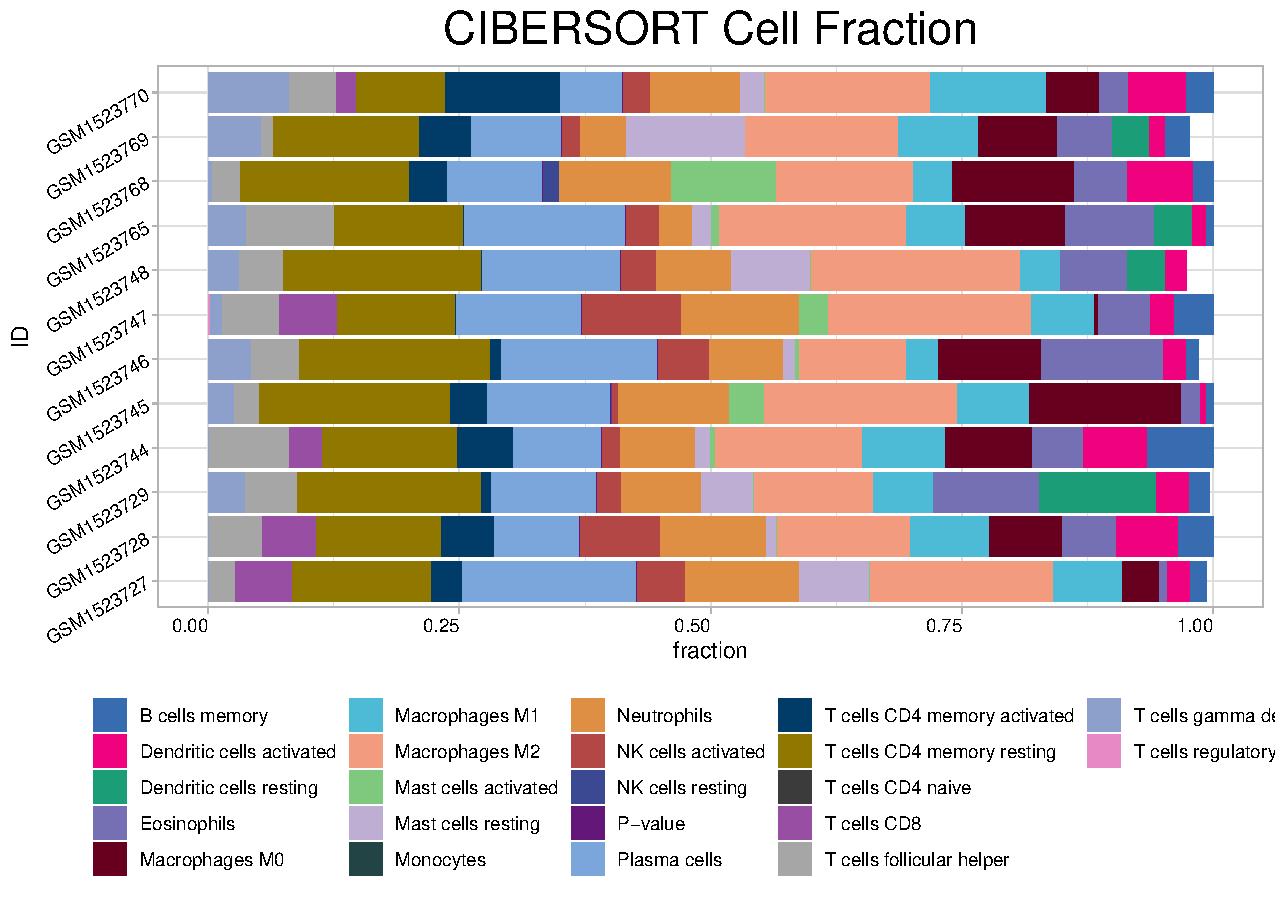
\includegraphics{tme-deconvolution_files/figure-latex/unnamed-chunk-7-1.pdf}

\hypertarget{method-2-epic}{%
\section{Method 2: EPIC}\label{method-2-epic}}

\begin{Shaded}
\begin{Highlighting}[]
\CommentTok{\# help(deconvo\_epic)}
\NormalTok{epic}\OtherTok{\textless{}{-}}\FunctionTok{deconvo\_tme}\NormalTok{(}\AttributeTok{eset =}\NormalTok{ eset\_acrg, }\AttributeTok{method =} \StringTok{"epic"}\NormalTok{, }\AttributeTok{arrays =} \ConstantTok{TRUE}\NormalTok{)}
\end{Highlighting}
\end{Shaded}

\begin{verbatim}
## 
## >>> Running EPIC
\end{verbatim}

\begin{verbatim}
## Warning in IOBR::EPIC(bulk = eset, reference = ref, mRNA_cell = NULL, scaleExprs = TRUE): The optimization didn't fully converge for some samples:
## GSM1523744; GSM1523746; GSM1523781; GSM1523786
##  - check fit.gof for the convergeCode and convergeMessage
\end{verbatim}

\begin{verbatim}
## Warning in IOBR::EPIC(bulk = eset, reference = ref, mRNA_cell = NULL, scaleExprs
## = TRUE): mRNA_cell value unknown for some cell types: CAFs, Endothelial - using
## the default value of 0.4 for these but this might bias the true cell proportions
## from all cell types.
\end{verbatim}

\begin{Shaded}
\begin{Highlighting}[]
\FunctionTok{head}\NormalTok{(epic)}
\end{Highlighting}
\end{Shaded}

\begin{verbatim}
## # A tibble: 6 x 9
##   ID      Bcells_EPIC CAFs_EPIC CD4_Tcells_EPIC CD8_Tcells_EPIC Endothelial_EPIC
##   <chr>         <dbl>     <dbl>           <dbl>           <dbl>            <dbl>
## 1 GSM152~      0.0292   0.00888           0.145          0.0756           0.0876
## 2 GSM152~      0.0293   0.0109            0.159          0.0745           0.0954
## 3 GSM152~      0.0308   0.0106            0.149          0.0732           0.0941
## 4 GSM152~      0.0273   0.0108            0.145          0.0704           0.0860
## 5 GSM152~      0.0280   0.0111            0.151          0.0707           0.0928
## 6 GSM152~      0.0320   0.00958           0.148          0.0716           0.0907
## # i 3 more variables: Macrophages_EPIC <dbl>, NKcells_EPIC <dbl>,
## #   otherCells_EPIC <dbl>
\end{verbatim}

\hypertarget{method-3-mcpcounter}{%
\section{Method 3: MCPcounter}\label{method-3-mcpcounter}}

\begin{Shaded}
\begin{Highlighting}[]
\NormalTok{mcp}\OtherTok{\textless{}{-}}\FunctionTok{deconvo\_tme}\NormalTok{(}\AttributeTok{eset =}\NormalTok{ eset\_acrg, }\AttributeTok{method =} \StringTok{"mcpcounter"}\NormalTok{)}
\end{Highlighting}
\end{Shaded}

\begin{verbatim}
## 
## >>> Running MCP-counter
\end{verbatim}

\begin{Shaded}
\begin{Highlighting}[]
\FunctionTok{head}\NormalTok{(mcp)}
\end{Highlighting}
\end{Shaded}

\begin{verbatim}
## # A tibble: 6 x 11
##   ID         T_cells_MCPcounter CD8_T_cells_MCPcounter Cytotoxic_lymphocytes_M~1
##   <chr>                   <dbl>                  <dbl>                     <dbl>
## 1 GSM1523727               1.47                  1.11                       1.33
## 2 GSM1523728               1.53                  1.05                       1.60
## 3 GSM1523729               1.47                  1.07                       1.37
## 4 GSM1523744               1.46                  1.02                       1.44
## 5 GSM1523745               1.51                  1.10                       1.49
## 6 GSM1523746               1.51                  0.992                      1.40
## # i abbreviated name: 1: Cytotoxic_lymphocytes_MCPcounter
## # i 7 more variables: B_lineage_MCPcounter <dbl>, NK_cells_MCPcounter <dbl>,
## #   Monocytic_lineage_MCPcounter <dbl>,
## #   Myeloid_dendritic_cells_MCPcounter <dbl>, Neutrophils_MCPcounter <dbl>,
## #   Endothelial_cells_MCPcounter <dbl>, Fibroblasts_MCPcounter <dbl>
\end{verbatim}

\hypertarget{method-4-xcell}{%
\section{Method 4: xCELL}\label{method-4-xcell}}

\begin{Shaded}
\begin{Highlighting}[]
\NormalTok{xcell}\OtherTok{\textless{}{-}}\FunctionTok{deconvo\_tme}\NormalTok{(}\AttributeTok{eset =}\NormalTok{ eset\_acrg, }\AttributeTok{method =} \StringTok{"xcell"}\NormalTok{, }\AttributeTok{arrays =} \ConstantTok{TRUE}\NormalTok{)}
\end{Highlighting}
\end{Shaded}

\begin{Shaded}
\begin{Highlighting}[]
\FunctionTok{head}\NormalTok{(xcell)}
\end{Highlighting}
\end{Shaded}

\begin{verbatim}
## # A tibble: 6 x 68
##   ID         aDC_xCell Adipocytes_xCell Astrocytes_xCell `B-cells_xCell`
##   <chr>          <dbl>            <dbl>            <dbl>           <dbl>
## 1 GSM1523727  4.78e-19          0.0250          0                 0     
## 2 GSM1523728  9.41e- 2          0.00433         7.70e- 3          0     
## 3 GSM1523729  1.02e- 1          0.0789          2.04e- 2          0     
## 4 GSM1523744  7.88e- 2          0.0538          4.82e-18          0.0126
## 5 GSM1523745  9.02e- 2          0.0136          1.93e- 2          0     
## 6 GSM1523746  3.40e- 2          0.0331          9.22e- 2          0     
## # i 63 more variables: Basophils_xCell <dbl>,
## #   `CD4+_memory_T-cells_xCell` <dbl>, `CD4+_naive_T-cells_xCell` <dbl>,
## #   `CD4+_T-cells_xCell` <dbl>, `CD4+_Tcm_xCell` <dbl>, `CD4+_Tem_xCell` <dbl>,
## #   `CD8+_naive_T-cells_xCell` <dbl>, `CD8+_T-cells_xCell` <dbl>,
## #   `CD8+_Tcm_xCell` <dbl>, `CD8+_Tem_xCell` <dbl>, cDC_xCell <dbl>,
## #   Chondrocytes_xCell <dbl>, `Class-switched_memory_B-cells_xCell` <dbl>,
## #   CLP_xCell <dbl>, CMP_xCell <dbl>, DC_xCell <dbl>, ...
\end{verbatim}

\hypertarget{method-5-estimate}{%
\section{Method 5: ESTIMATE}\label{method-5-estimate}}

\begin{Shaded}
\begin{Highlighting}[]
\NormalTok{estimate}\OtherTok{\textless{}{-}}\FunctionTok{deconvo\_tme}\NormalTok{(}\AttributeTok{eset =}\NormalTok{ eset\_acrg, }\AttributeTok{method =} \StringTok{"estimate"}\NormalTok{)}
\end{Highlighting}
\end{Shaded}

\begin{verbatim}
## [1] "Merged dataset includes 9940 genes (472 mismatched)."
## [1] "1 gene set: StromalSignature  overlap= 136"
## [1] "2 gene set: ImmuneSignature  overlap= 138"
\end{verbatim}

\begin{Shaded}
\begin{Highlighting}[]
\FunctionTok{head}\NormalTok{(estimate)}
\end{Highlighting}
\end{Shaded}

\begin{verbatim}
## # A tibble: 6 x 5
##   ID         StromalScore_estimate ImmuneScore_estimate ESTIMATEScore_estimate
##   <chr>                      <dbl>                <dbl>                  <dbl>
## 1 GSM1523727                -1250.                 268.                 -982. 
## 2 GSM1523728                  197.                1334.                 1531. 
## 3 GSM1523729                 -111.                 822.                  711. 
## 4 GSM1523744                 -119.                 662.                  544. 
## 5 GSM1523745                  324.                1015.                 1339. 
## 6 GSM1523746                 -594.                 621.                   27.0
## # i 1 more variable: TumorPurity_estimate <dbl>
\end{verbatim}

\hypertarget{method-6-timer}{%
\section{Method 6: TIMER}\label{method-6-timer}}

\begin{Shaded}
\begin{Highlighting}[]
\NormalTok{timer}\OtherTok{\textless{}{-}}\FunctionTok{deconvo\_tme}\NormalTok{(}\AttributeTok{eset =}\NormalTok{ eset\_acrg, }\AttributeTok{method =} \StringTok{"timer"}\NormalTok{, }\AttributeTok{group\_list =} \FunctionTok{rep}\NormalTok{(}\StringTok{"stad"}\NormalTok{,}\FunctionTok{dim}\NormalTok{(eset\_acrg)[}\DecValTok{2}\NormalTok{]))}
\end{Highlighting}
\end{Shaded}

\begin{verbatim}
## [1] "Outlier genes: AGR2 B2M COL1A2 COL3A1 COX2 CYAT1 EEF1A1 EIF1 FTH1 GKN1 HUWE1 IGK IGLC1 LIPF LOC101060363 LOC101928826 MIR8071-2 ND4 PABPC1 PABPC3 PGA4 RPL13AP5 RPL37 RPL37A RPL41 RPL7 RPS10 RPS16 RPS17 RPS18 RPS19 S100A6 S100A9 SH3KBP1 SNORD24 SNORD42A SNORD54 SNORD73A SPINK1 SPINK4 TFF1 UQCRFS1"
\end{verbatim}

\begin{Shaded}
\begin{Highlighting}[]
\FunctionTok{head}\NormalTok{(timer)}
\end{Highlighting}
\end{Shaded}

\begin{verbatim}
## # A tibble: 6 x 7
##   ID         B_cell_TIMER T_cell_CD4_TIMER T_cell_CD8_TIMER Neutrophil_TIMER
##   <chr>             <dbl>            <dbl>            <dbl>            <dbl>
## 1 GSM1523727        0.104            0.128            0.183            0.108
## 2 GSM1523728        0.103            0.130            0.192            0.118
## 3 GSM1523729        0.106            0.130            0.190            0.110
## 4 GSM1523744        0.101            0.126            0.187            0.111
## 5 GSM1523745        0.104            0.127            0.191            0.116
## 6 GSM1523746        0.105            0.129            0.192            0.111
## # i 2 more variables: Macrophage_TIMER <dbl>, DC_TIMER <dbl>
\end{verbatim}

\hypertarget{method-7-quantiseq}{%
\section{Method 7: quanTIseq}\label{method-7-quantiseq}}

\begin{Shaded}
\begin{Highlighting}[]
\NormalTok{quantiseq}\OtherTok{\textless{}{-}}\FunctionTok{deconvo\_tme}\NormalTok{(}\AttributeTok{eset =}\NormalTok{ eset\_acrg, }\AttributeTok{tumor =} \ConstantTok{TRUE}\NormalTok{, }\AttributeTok{arrays =} \ConstantTok{TRUE}\NormalTok{, }\AttributeTok{scale\_mrna =} \ConstantTok{TRUE}\NormalTok{, }\AttributeTok{method =} \StringTok{"quantiseq"}\NormalTok{)}
\end{Highlighting}
\end{Shaded}

\begin{verbatim}
## 
## Running quanTIseq deconvolution module
\end{verbatim}

\begin{verbatim}
## Gene expression normalization and re-annotation (arrays: TRUE)
\end{verbatim}

\begin{verbatim}
## Removing 17 genes with high expression in tumors
\end{verbatim}

\begin{verbatim}
## Signature genes found in data set: 152/153 (99.35%)
\end{verbatim}

\begin{verbatim}
## Mixture deconvolution (method: lsei)
\end{verbatim}

\begin{verbatim}
## Deconvolution sucessful!
\end{verbatim}

\begin{Shaded}
\begin{Highlighting}[]
\FunctionTok{head}\NormalTok{(quantiseq)}
\end{Highlighting}
\end{Shaded}

\begin{verbatim}
## # A tibble: 6 x 12
##   ID         B_cells_quantiseq Macrophages_M1_quantiseq Macrophages_M2_quantiseq
##   <chr>                  <dbl>                    <dbl>                    <dbl>
## 1 GSM1523727            0.0983                   0.0510                   0.0598
## 2 GSM1523728            0.0967                   0.0795                   0.0607
## 3 GSM1523729            0.102                    0.0450                   0.0758
## 4 GSM1523744            0.0954                   0.0725                   0.0579
## 5 GSM1523745            0.0991                   0.0669                   0.0613
## 6 GSM1523746            0.105                    0.0453                   0.0662
## # i 8 more variables: Monocytes_quantiseq <dbl>, Neutrophils_quantiseq <dbl>,
## #   NK_cells_quantiseq <dbl>, T_cells_CD4_quantiseq <dbl>,
## #   T_cells_CD8_quantiseq <dbl>, Tregs_quantiseq <dbl>,
## #   Dendritic_cells_quantiseq <dbl>, Other_quantiseq <dbl>
\end{verbatim}

\begin{Shaded}
\begin{Highlighting}[]
\NormalTok{res}\OtherTok{\textless{}{-}}\FunctionTok{cell\_bar\_plot}\NormalTok{(}\AttributeTok{input =}\NormalTok{ quantiseq[}\DecValTok{1}\SpecialCharTok{:}\DecValTok{12}\NormalTok{, ], }\AttributeTok{title =} \StringTok{"quanTIseq Cell Fraction"}\NormalTok{)}
\end{Highlighting}
\end{Shaded}

\begin{verbatim}
## There are seven categories you can choose: box, continue2, continue, random, heatmap, heatmap3, tidyheatmap
\end{verbatim}

\begin{verbatim}
## >>>>=== Palette option for random: 1: palette1; 2: palette2; 3: palette3;  4: palette4
\end{verbatim}

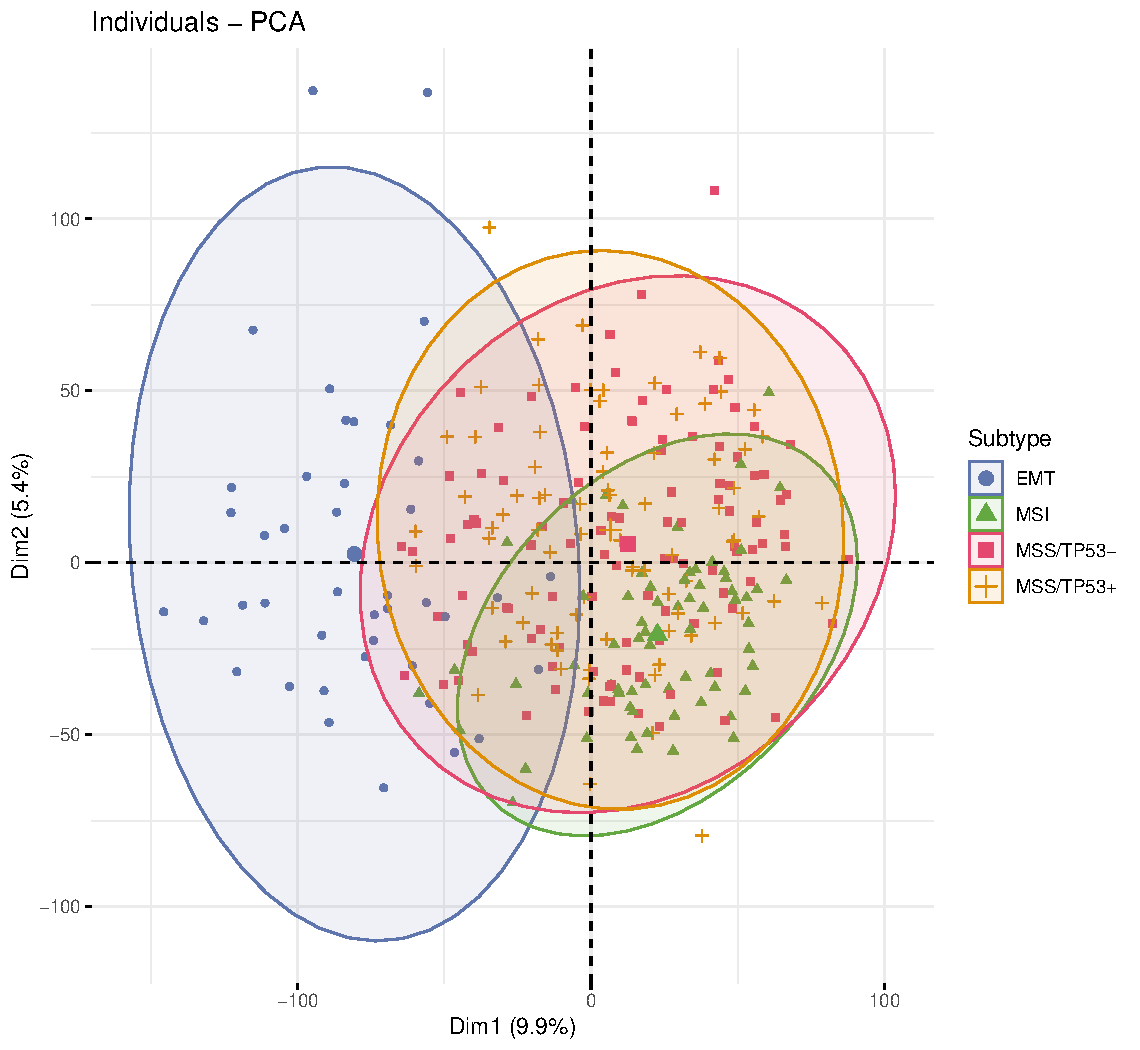
\includegraphics{tme-deconvolution_files/figure-latex/unnamed-chunk-14-1.pdf}

\hypertarget{method-8-ips}{%
\section{Method 8: IPS}\label{method-8-ips}}

\begin{Shaded}
\begin{Highlighting}[]
\NormalTok{ips}\OtherTok{\textless{}{-}}\FunctionTok{deconvo\_tme}\NormalTok{(}\AttributeTok{eset =}\NormalTok{ eset\_acrg, }\AttributeTok{method =} \StringTok{"ips"}\NormalTok{, }\AttributeTok{plot=} \ConstantTok{FALSE}\NormalTok{)}
\FunctionTok{head}\NormalTok{(ips)}
\end{Highlighting}
\end{Shaded}

\begin{verbatim}
## # A tibble: 6 x 7
##   ID         MHC_IPS EC_IPS SC_IPS  CP_IPS AZ_IPS IPS_IPS
##   <chr>        <dbl>  <dbl>  <dbl>   <dbl>  <dbl>   <dbl>
## 1 GSM1523727    2.25  0.404 -0.192  0.220    2.68       9
## 2 GSM1523728    2.37  0.608 -0.578 -0.234    2.17       7
## 3 GSM1523729    2.10  0.480 -0.322  0.0993   2.36       8
## 4 GSM1523744    2.12  0.535 -0.333  0.0132   2.34       8
## 5 GSM1523745    1.91  0.559 -0.479  0.0880   2.08       7
## 6 GSM1523746    1.94  0.458 -0.346  0.261    2.31       8
\end{verbatim}

\hypertarget{combination-of-above-deconvolution-results}{%
\section{Combination of above deconvolution results}\label{combination-of-above-deconvolution-results}}

\begin{Shaded}
\begin{Highlighting}[]
\NormalTok{tme\_combine}\OtherTok{\textless{}{-}}\NormalTok{cibersort }\SpecialCharTok{\%\textgreater{}\%} 
  \FunctionTok{inner\_join}\NormalTok{(.,mcp,}\AttributeTok{by       =} \StringTok{"ID"}\NormalTok{) }\SpecialCharTok{\%\textgreater{}\%} 
  \FunctionTok{inner\_join}\NormalTok{(.,xcell,}\AttributeTok{by     =} \StringTok{"ID"}\NormalTok{) }\SpecialCharTok{\%\textgreater{}\%}
  \FunctionTok{inner\_join}\NormalTok{(.,epic,}\AttributeTok{by      =} \StringTok{"ID"}\NormalTok{) }\SpecialCharTok{\%\textgreater{}\%} 
  \FunctionTok{inner\_join}\NormalTok{(.,estimate,}\AttributeTok{by  =} \StringTok{"ID"}\NormalTok{) }\SpecialCharTok{\%\textgreater{}\%} 
  \FunctionTok{inner\_join}\NormalTok{(.,timer,}\AttributeTok{by     =} \StringTok{"ID"}\NormalTok{) }\SpecialCharTok{\%\textgreater{}\%} 
  \FunctionTok{inner\_join}\NormalTok{(.,quantiseq,}\AttributeTok{by =} \StringTok{"ID"}\NormalTok{) }\SpecialCharTok{\%\textgreater{}\%} 
  \FunctionTok{inner\_join}\NormalTok{(.,ips,}\AttributeTok{by       =} \StringTok{"ID"}\NormalTok{)}
\FunctionTok{dim}\NormalTok{(tme\_combine)}
\end{Highlighting}
\end{Shaded}

\begin{verbatim}
## [1]  50 138
\end{verbatim}

If you use this package in your work, please cite both our package and the method(s) you are using.

Licenses of the deconvolution methods

\href{https://cibersort.stanford.edu/}{CIBERSORT}; free for non-commerical use only; Newman, A. M., Liu, C. L., Green, M. R., Gentles, A. J., Feng, W., Xu, Y., \ldots{} Alizadeh, A. A. (2015). Robust enumeration of cell subsets from tissue expression profiles. Nature Methods, 12(5), 453--457. \url{https://doi.org/10.1038/nmeth.3337};

\href{https://bioinformatics.mdanderson.org/public-software/estimate/}{ESTIMATE}; free (\href{https://bioinformatics.mdanderson.org/estimate/}{GPL2.0}); Vegesna R, Kim H, Torres-Garcia W, \ldots, Verhaak R. (2013). Inferring tumour purity and stromal and immune cell admixture from expression data. Nature Communications 4, 2612. \url{http://doi.org/10.1038/ncomms3612};

\href{http://icbi.at/software/quantiseq/doc/index.html}{quanTIseq}; free (\href{https://github.com/icbi-lab/immunedeconv/blob/master/LICENSE.md}{BSD}); Finotello, F., Mayer, C., Plattner, C., Laschober, G., Rieder, D., Hackl, H., \ldots, Sopper, S. (2019). Molecular and pharmacological modulators of the tumor immune contexture revealed by deconvolution of RNA-seq data. Genome medicine, 11(1), 34. \url{https://doi.org/10.1186/s13073-019-0638-6};

\href{http://cistrome.org/TIMER/}{TIMER}; free (\href{http://cistrome.org/TIMER/download.html}{GPL 2.0}); Li, B., Severson, E., Pignon, J.-C., Zhao, H., Li, T., Novak, J., \ldots{} Liu, X. S. (2016). Comprehensive analyses of tumor immunity: implications for cancer immunotherapy. Genome Biology, 17(1), 174. \url{https://doi.org/10.1186/s13059-016-1028-7};

\href{https://github.com/icbi-lab/Immunophenogram}{IPS}; free (\href{https://github.com/icbi-lab/Immunophenogram/blob/master/LICENSE}{BSD}); P. Charoentong et al., Pan-cancer Immunogenomic Analyses Reveal Genotype-Immunophenotype Relationships and Predictors of Response to Checkpoint Blockade. Cell Reports 18, 248-262 (2017). \url{https://doi.org/10.1016/j.celrep.2016.12.019};

\href{https://github.com/ebecht/MCPcounter}{MCPCounter}; free (\href{https://github.com/ebecht/MCPcounter/blob/master/Source/License}{GPL 3.0}); Becht, E., Giraldo, N. A., Lacroix, L., Buttard, B., Elarouci, N., Petitprez, F., \ldots{} de Reyniès, A. (2016). Estimating the population abundance of tissue-infiltrating immune and stromal cell populations using gene expression. Genome Biology, 17(1), 218. \url{https://doi.org/10.1186/s13059-016-1070-5};

\href{http://xcell.ucsf.edu/}{xCell}; free (\href{https://github.com/dviraran/xCell/blob/master/DESCRIPTION}{GPL 3.0}); Aran, D., Hu, Z., \& Butte, A. J. (2017). xCell: digitally portraying the tissue cellular heterogeneity landscape. Genome Biology, 18(1), 220. \url{https://doi.org/10.1186/s13059-017-1349-1};

\href{https://gfellerlab.shinyapps.io/EPIC_1-1/}{EPIC}; free for non-commercial use only (\href{https://github.com/GfellerLab/EPIC/blob/master/LICENSE}{Academic License}); Racle, J., de Jonge, K., Baumgaertner, P., Speiser, D. E., \& Gfeller, D. (2017). Simultaneous enumeration of cancer and immune cell types from bulk tumor gene expression data. ELife, 6, e26476. \url{https://doi.org/10.7554/eLife.26476};

\href{http://www.bioconductor.org/packages/release/bioc/html/GSVA.html}{GSVA} free (\href{https://github.com/rcastelo/GSVA}{GPL (\textgreater= 2)}) Hänzelmann S, Castelo R, Guinney J (2013). ``GSVA: gene set variation analysis for microarray and RNA-Seq data.'' BMC Bioinformatics, 14, 7. doi: 10.1186/1471-2105-14-7, \url{http://www.biomedcentral.com/1471-2105/14/7} \textbar{}

\hypertarget{references-1}{%
\chapter{\texorpdfstring{\textbf{References}}{References}}\label{references-1}}

If IOBR R package is utilized in your published research, please cite:

Zeng D, Ye Z, Shen R, Yu G, Wu J, Xiong Y,\ldots, Liao W (2021) \textbf{IOBR}: Multi-Omics Immuno-Oncology Biological Research to Decode Tumor Microenvironment and Signatures. \emph{Frontiers in Immunology}. 12:687975. \href{https://www.frontiersin.org/articles/10.3389/fimmu.2021.687975/full}{doi: 10.3389/fimmu.2021.687975}

\hypertarget{tme-deconvolution-1}{%
\section{TME deconvolution}\label{tme-deconvolution-1}}

Please cite the following papers appropriately for TME deconvolution algorithm if used:

\textbf{CIBERSORT}: Newman, A. M., Liu, C. L., Green, M. R., Gentles, A. J., Feng, W., Xu, Y., \ldots{} Alizadeh, A. A. (2015). Robust enumeration of cell subsets from tissue expression profiles. Nature Methods, 12(5), 453--457. \url{https://doi.org/10.1038/nmeth.3337}

\textbf{ESTIMATE}: Vegesna R, Kim H, Torres-Garcia W, \ldots, Verhaak R.*(2013). Inferring tumour purity and stromal and immune cell admixture from expression data. Nature Communications 4, 2612. \url{http://doi.org/10.1038/ncomms3612}

\textbf{quanTIseq}: Finotello, F., Mayer, C., Plattner, C., Laschober, G., Rieder, D., Hackl, H., \ldots, Sopper, S.* (2019). Molecular and pharmacological modulators of the tumor immune contexture revealed by deconvolution of RNA-seq data. Genome medicine, 11(1), 34. \url{https://doi.org/10.1186/s13073-019-0638-6}

\textbf{TIMER}: Li, B., Severson, E., Pignon, J.-C., Zhao, H., Li, T., Novak, J., \ldots{} Liu, X. S.* (2016). Comprehensive analyses of tumor immunity: implications for cancer immunotherapy. Genome Biology, 17(1), 174.

\textbf{IPS}: P. Charoentong et al.*, Pan-cancer Immunogenomic Analyses Reveal Genotype-Immunophenotype Relationships and Predictors of Response to Checkpoint Blockade. Cell Reports 18, 248-262 (2017). \url{https://doi.org/10.1016/j.celrep.2016.12.019}

\textbf{MCPCounter}: Becht, E., Giraldo, N. A., Lacroix, L., Buttard, B., Elarouci, N., Petitprez, F., \ldots{} de Reyniès, A*. (2016). Estimating the population abundance of tissue-infiltrating immune and stromal cell populations using gene expression. Genome Biology, 17(1), 218. \url{https://doi.org/10.1186/s13059-016-1070-5}

\textbf{xCell}: Aran, D., Hu, Z., \& Butte, A. J.* (2017). xCell: digitally portraying the tissue cellular heterogeneity landscape. Genome Biology, 18(1), 220. \url{https://doi.org/10.1186/s13059-017-1349-1}

\textbf{EPIC}: Racle, J., de Jonge, K., Baumgaertner, P., Speiser, D. E., \& Gfeller, D*. (2017). Simultaneous enumeration of cancer and immune cell types from bulk tumor gene expression data. ELife, 6, e26476. \url{https://doi.org/10.7554/eLife.26476}

\hypertarget{tme-signatures}{%
\section{TME Signatures}\label{tme-signatures}}

For signature score estimation, please cite corresponding literature below:

\textbf{ssgsea}: Barbie, D.A. et al (2009). Systematic RNA interference reveals that oncogenic KRAS-driven cancers require TBK1. Nature, 462(5):108-112.

\textbf{gsva}: Hänzelmann, S., Castelo, R. and Guinney, J. (2013). GSVA: Gene set variation analysis for microarray and RNA-Seq data. BMC Bioinformatics, 14(1):7.

\textbf{zscore}: Lee, E. et al (2008). Inferring pathway activity toward precise disease classification. PLoS Comp Biol, 4(11):e1000217.

\hypertarget{data-sets}{%
\section{Data sets}\label{data-sets}}

For the datasets enrolled in IOBR, please cite the data sources:

\textbf{UCSCXena}: Wang et al.,et al (2019). The UCSCXenaTools R package: a toolkit for accessing genomics data from UCSC Xena platform, from cancer multi-omics to single-cell RNA-seq. Journal of Open Source Software, 4(40), 1627

\textbf{TLSscore}: Helmink BA, Reddy SM, Gao J, et al.~B cells and tertiary lymphoid structures promote immunotherapy response. Nature. 2020 Jan;577(7791):549-555.

\textbf{IMvigor210 immuntherapy cohort}: Mariathasan S, Turley SJ, Nickles D, et al.~TGFβ attenuates tumour response to PD-L1 blockade by contributing to exclusion of T cells. Nature. 2018 Feb 22;554(7693):544-548.
\textbf{HCP5}: Kulski, J.K. Long Noncoding RNA HCP5, a Hybrid HLA Class I Endogenous Retroviral Gene: Structure, Expression, and Disease Associations. Cells 2019, 8, 480.

\textbf{HCP5}: Li, Y., Jiang, T., Zhou, W. et al.~Pan-cancer characterization of immune-related lncRNAs identifies potential oncogenic biomarkers. Nat Commun 11, 1000 (2020).
HCP5: Sun J, Zhang Z, Bao S, et alIdentification of tumor immune infiltration-associated lncRNAs for improving prognosis and immunotherapy response of patients with non-small cell lung cancerJournal for ImmunoTherapy of Cancer 2020;8:e000110.

\textbf{LINC00657}: Feng Q, Zhang H, Yao D, Chen WD, Wang YD. Emerging Role of Non-Coding RNAs in Esophageal Squamous Cell Carcinoma. Int J Mol Sci. 2019 Dec 30;21(1):258. doi: 10.3390/ijms21010258.

\textbf{LINC00657}: Qin X, Zhou M, Lv H, Mao X, Li X, Guo H, Li L, Xing H. Long noncoding RNA LINC00657 inhibits cervical cancer development by sponging miR-20a-5p and targeting RUNX3. Cancer Lett. 2020 Oct 28:S0304-3835(20)30578-4. doi: 10.1016/j.canlet.2020.10.044.
\textbf{LINC00657}: Zhang XM, Wang J, Liu ZL, Liu H, Cheng YF, Wang T. LINC00657/miR-26a-5p/CKS2 ceRNA network promotes the growth of esophageal cancer cells via the MDM2/p53/Bcl2/Bax pathway. Biosci Rep.~2020;40(6):BSR20200525.

\textbf{TCGA-STAD}: Cancer Genome Atlas Research Network. Comprehensive molecular characterization of gastric adenocarcinoma. Nature. 2014 Sep 11;513(7517):202-9. doi: 10.1038/nature13480.
TCGA.STAD MAF data: \url{https://api.gdc.cancer.gov/data/c06465a3-50e7-46f7-b2dd-7bd654ca206b}

\hypertarget{others}{%
\section{Others}\label{others}}

\begin{enumerate}
\def\labelenumi{\arabic{enumi}.}
\item
  Newman, A. M., Liu, C. L., Green, M. R., Gentles, A. J., Feng, W., Xu, Y., \ldots{} Alizadeh, A. A. (2015). Robust enumeration of cell subsets from tissue expression profiles. Nature Methods, 12(5), 453--457.
\item
  Vegesna R, Kim H, Torres-Garcia W, \ldots, Verhaak R.*(2013). Inferring tumour purity and stromal and immune cell admixture from expression data. Nature Communications 4, 2612.
\item
  Rieder, D., Hackl, H., \ldots, Sopper, S.* (2019). Molecular and pharmacological modulators of the tumor immune contexture revealed by deconvolution of RNA-seq data. Genome medicine, 11(1), 34.
\item
  Li, B., Severson, E., Pignon, J.-C., Zhao, H., Li, T., Novak, J., \ldots{} Liu, X. S.* (2016). Comprehensive analyses of tumor immunity: implications for cancer immunotherapy. Genome Biology, 17(1), 174.
\item
  P. Charoentong et al.*, Pan-cancer Immunogenomic Analyses Reveal Genotype-Immunophenotype Relationships and Predictors of Response to Checkpoint Blockade. Cell Reports 18, 248-262 (2017).
\item
  Becht, E., Giraldo, N. A., Lacroix, L., Buttard, B., Elarouci, N., Petitprez, F., \ldots{} de Reyniès, A*. (2016). Estimating the population abundance of tissue-infiltrating immune and stromal cell populations using gene expression. Genome Biology, 17(1), 218.
\item
  Aran, D., Hu, Z., \& Butte, A. J.* (2017). xCell: digitally portraying the tissue cellular heterogeneity landscape. Genome Biology, 18(1), 220.
\item
  Racle, J., de Jonge, K., Baumgaertner, P., Speiser, D. E., \& Gfeller, D*. (2017). Simultaneous enumeration of cancer and immune cell types from bulk tumor gene expression data. ELife, 6, e26476.
\item
  Barbie, D.A. et al (2009). Systematic RNA interference reveals that oncogenic KRAS-driven cancers require TBK1. Nature, 462(5):108-112.
\item
  Hänzelmann, S., Castelo, R. and Guinney, J. (2013). GSVA: Gene set variation analysis for microarray and RNA-Seq data. BMC Bioinformatics, 14(1):7.
\item
  Lee, E. et al (2008). Inferring pathway activity toward precise disease classification. PLoS Comp Biol, 4(11):e1000217.
\item
  Wang et al.,et al (2019). The UCSCXenaTools R package: a toolkit for accessing genomics data from UCSC Xena platform, from cancer multi-omics to single-cell RNA-seq. Journal of Open Source Software, 4(40), 1627
\item
  Helmink BA, Reddy SM, Gao J, et al.~B cells and tertiary lymphoid structures promote immunotherapy response. Nature. 2020 Jan;577(7791):549-555.
\item
  Mariathasan S, Turley SJ, Nickles D, et al.~TGFβ attenuates tumour response to PD-L1 blockade by contributing to exclusion of T cells. Nature. 2018 Feb 22;554(7693):544-548.
\item
  Kulski, J.K. Long Noncoding RNA HCP5, a Hybrid HLA Class I Endogenous Retroviral Gene: Structure, Expression, and Disease Associations. Cells 2019, 8, 480.
\item
  Li, Y., Jiang, T., Zhou, W. et al.~Pan-cancer characterization of immune-related lncRNAs identifies potential oncogenic biomarkers. Nat Commun 11, 1000 (2020).
\item
  Sun J, Zhang Z, Bao S, et alIdentification of tumor immune infiltration-associated lncRNAs for improving prognosis and immunotherapy response of patients with non-small cell lung cancerJournal for ImmunoTherapy of Cancer 2020;8:e000110.
\item
  Feng Q, Zhang H, Yao D, Chen WD, Wang YD. Emerging Role of Non-Coding RNAs in Esophageal Squamous Cell Carcinoma. Int J Mol Sci. 2019 Dec 30;21(1):258. doi: 10.3390/ijms21010258.
\item
  Qin X, Zhou M, Lv H, Mao X, Li X, Guo H, Li L, Xing H. Long noncoding RNA LINC00657 inhibits cervical cancer development by sponging miR-20a-5p and targeting RUNX3. Cancer Lett. 2020 Oct
\item
  Zhang XM, Wang J, Liu ZL, Liu H, Cheng YF, Wang T. LINC00657/miR-26a-5p/CKS2 ceRNA network promotes the growth of esophageal cancer cells via the MDM2/p53/Bcl2/Bax pathway. Biosci Rep.~2020;40(6):BSR20200525.
\item
  Cancer Genome Atlas Research Network. Comprehensive molecular characterization of gastric adenocarcinoma. Nature. 2014 Sep 11;513(7517):202-9. doi: 10.1038/nature13480.
\end{enumerate}

  \bibliography{book.bib,packages.bib}

\end{document}
